\usepackage[english]{babel}
%\usepackage[english,french]{babel}
\usepackage{algpseudocode}
\usepackage{algorithm}
\usepackage{amsmath}
\usepackage{amsfonts}
\usepackage{mathtools}
\usepackage{rotating}
\usepackage{multicol}
\usepackage{color}
\usepackage{verbatim}
\usepackage{hyperref}
\usepackage{float}
\usepackage{listings}
\lstset{
  basicstyle=\ttfamily,
  columns=fullflexible,
  frame=single,
  breaklines=true,
  postbreak=\mbox{\textcolor{red}{$\hookrightarrow$}\space},
}
%\usepackage{cprotect}
\usepackage{fancyvrb}
\usepackage{color}
%for subfigure using ?
\usepackage{graphicx}
\usepackage{caption}
\usepackage{subcaption}
\usepackage{makeidx}
%\usepackage{amsmath}
\usepackage{amssymb}

\makeindex


\DeclareMathOperator*{\argmax}{arg\,max}

%\usepackage{subfigure}

%\usepackage{mathabx}
%\usepackage{amstext}
%\usepackage{amssymb}
%\usepackage{ae}


\setcounter{tocdepth}{4}
\setcounter{secnumdepth}{4}


%allow to break on / in texttt
\usepackage{xparse}
\ExplSyntaxOn
\NewDocumentCommand{\replace}{mmm}
 {
  \marian_replace:nnn {#1} {#2} {#3}
 }
\tl_new:N \l_marian_input_text_tl
\cs_new_protected:Npn \marian_replace:nnn #1 #2 #3
 {
  \tl_set:Nn \l_marian_input_text_tl { #1 }
  \tl_replace_all:Nnn \l_marian_input_text_tl { #2 } { #3 }
  \tl_use:N \l_marian_input_text_tl
 }
\ExplSyntaxOff
\let\OldTexttt\texttt
\renewcommand{\texttt}[1]{\OldTexttt{\replace{#1}{/}{/\allowbreak}}}
\let\Oldtt\tt
\renewcommand{\tt}[1]{\Oldtt{\replace{#1}{/}{/\allowbreak}}}

%---------------------------------------------
\newcommand{\CPP}{\mbox{\tt C\hspace{-0.05cm}\raisebox{0.2ex}{\small ++} }}
\newcommand{\SiftPP}{\mbox{\tt Sift\hspace{-0.05cm}\raisebox{0.2ex}{\small ++} }}


\newcommand{\tran}{\ensuremath {^{t} }}
\newcommand{\trans}{\ensuremath {\; ^{t} \!}}
\newcommand{\transs}{\ensuremath {\;\;  ^{t} \!\!}}
\newcommand{\transss}{\ensuremath {\;\;\;   ^{t} \!\!\!}}


\newcommand{\transL}{{\transs L}}
\newcommand{\transK}{{\transs K}}
\newcommand{\transX}{{\transs X}}
\newcommand{\transY}{{\transs Y}}

\newcommand{\transLm}{\ensuremath {\transs L^m}}
\newcommand{\transKm}{\ensuremath {\transs K^m}}
\newcommand{\KmtKm}{\ensuremath { K^m \, \transKm}}
\newcommand{\LmtLm}{\ensuremath { L^m \, \transLm}}

\newcommand{\KTH}{\ensuremath {^{th}}}
\newcommand{\EME}{\ensuremath {^{i\grave eme}}}
\newcommand{\ETer}{\ensuremath {\mathcal T}}
\newcommand{\EIm}{\ensuremath {{\mathcal I}_k}}
\newcommand{\EPx}{\ensuremath{{\mathcal E}_{px}}}

\newcommand{\FPx}{\ensuremath{{\mathcal F}_{px}}}

\newcommand{\Ok}{\ensuremath{{\mathcal O}_{k}}}

\newcommand{\Ess}{\ensuremath{{\mathcal E}}}
\newcommand{\Interpol}{\ensuremath {\mathcal I}}
\newcommand{\KernI}{\ensuremath {\mathcal K}}

\newcommand{\DimPx}{\ensuremath{D_{px}}}

\newcommand{\PiI}{\ensuremath{\dot{\pi}}}
\newcommand{\PxMoy}{\ensuremath{\tilde{P_x}}}
\newcommand{\PxZone}{\ensuremath{P_x^Z}}

\newcommand{\LP}{\ensuremath{{\mathcal L_P}}}
\newcommand{\ChBit}{\ensuremath{{\mathcal B}}}

\newcommand{\RR}{\ensuremath{\mathbb{R}}}
\newcommand{\ZZ}{\ensuremath{\mathbb{Z}}}
\newcommand{\NN}{\ensuremath{\mathbb{N}}}
\newcommand{\Ind}{\ensuremath{\mathbb{I}^{nd}}}

\newcommand{\Ress}{\ensuremath{{\mathcal A}}}
\newcommand{\Reg}{\ensuremath{{\mathcal R}^{eg}}}
\newcommand{\Energ}{\ensuremath{{\mathcal E}}}
\newcommand{\Echant}{\ensuremath{{\mathcal E}}}
\newcommand{\PZero}{\ensuremath{{\mathcal P}^0}}
\newcommand{\SUn}{\ensuremath{{\mathcal S}^1}}

\newcommand{\DeltaI}{\ensuremath{\Delta^{\imath}}}
\DeclareMathOperator{\sinc}{sinc}

\newcommand{\DdSt}{\ensuremath{d^2}_{/\mathcal{S}^3}}
\newcommand{\DeuxExtre}{\ensuremath{\unrhd}}
%\newcommand{\DeuxExtre}{\ensuremath{\nabla}}
\newcommand{\RefFantome}{{\bf ?2Def?}}
\newcommand{\TOMODIF}[1]{\textcolor{red}{\textbf{#1}}}

\newcommand{\TOIMPROVE}[1]{\textcolor{red}{\textbf{Possible improvement (??)} : [#1]}}

\newcommand{\PourLecteurAverti}{{\Large \bf \emph{Ce paragraphe peut
facilement \^etre omis
en premi\`ere lecture.}}}
\newcommand{\COM}[1]

\newtheorem{proposal}{Proposal}

%  \verb|\|


\newcommand{\ELISE}
{\mbox{{\bf $\mathcal{E}$}\hspace{-0.15em}\raisebox{-0.4ex}{L}\hspace{-0.3em}\raisebox{0.3ex}{i}\raisebox{-0.4ex}{S}\raisebox{0.0ex}{e}}}

%\newcommand{\UNCLEAR}[1]{\textcolor{red}{\textbf{#1}}}
\newcommand{\UNCLEAR}{}
\newcommand{\ISITCLEAR}{}
\newcommand{\PPP}{MMVII}

\newcommand{\MmVii}
{
\ensuremath{ \mbox{
     {\bf $\mathcal{M}$}\hspace{-0.15em}\raisebox{-0.4ex}{$m$}\hspace{-0.3em}\raisebox{0.3ex}{$V$}\raisebox{-0.4ex}{$2$}
}}}

\newcommand{\CdPPP}{{\tt MMVII}}
\newcommand{\MMVIDIR}{{\tt MMVII-MainFolder/}}
\newcommand{\doxy}{\emph{doxygen}}
\newcommand{\MMNONE}{NONE}

%\includeonly{Methods/PoseGlobInit}
%\includeonly{Programmer/Interpolators}
%\includeonly{Methods/LidarImageRegistration}

%---------------------------------------------
\begin{document}
\selectlanguage{english}

%\title{MicMac, Apero, Pastis and Other Beverages. The documentation!}
\title{Project 2007}
%\author{MPD}

\maketitle

\tableofcontents


%###########################################################################################################
%###########################################################################################################
%---------------------------------------------- GENERATLITIES ----------------------------------------------
%###########################################################################################################
%###########################################################################################################

\part{Generalities}

\include{Generalities/Intro}
\chapter{Project management command}

%---------------------------------------------
%---------------------------------------------
%---------------------------------------------
\section{Readible file formats}

\subsection{Readible/Binary}

As photogrammetric pipeline is a complex process, made of several computation,
the result of each computation has to be writen in some files that
will be read at by next process. There is basically two familly of such files:

\begin{itemize}
   \item files that may have some interest to  be read or manipulated by human
         or other programm, in this case {\tt MMVII} standar tagged format
	 as {\tt xml} of {\tt json}; example of such file are calibration
	 or pose estimation;

   \item files that have probably low interest for human, and for efficiency 
         they are stored in binary format  (note that there exist also a
         text version of this binary format, note easy to read, but that facilitate
	   import export);
\end{itemize}

\subsection{Xml and Json files}

{\tt MMVII} offer the possibility to export data in two different tagged format : {\tt xml} and
{\tt json}. By default it's {\tt xml}, but this can be changed using mecanism descrined in \ref{UserParametrisation}.
Implicit conversion may appear in a near future for sharing files between user,
by the way it's recommanded that user make a choice once for all  to avoid any problem.

The folder {\tt MMVII-UseCaseDataSet/SampleFiles} contains examples
of files in {\tt xml} and {\tt json}. 

Note that {\tt xml} allows real coments and, for example, in the file {\tt Calib...xml}, they are used to
explicit  the meanin of distorsion parameters. As {\tt json} do not have
real comments, we use the special tags , for example in file
{\tt Calib...json} you can find {\tt "<!--comment6-->":"(X,0)"}
(corresponding to  {\tt <!--(X,0)-->} in {\tt xml}).

These file are made to be relatively easy to read. They can also be created or
modified easily by user or programm however there are some \emph{strict} rules to observe so that such
file remain valid . Starting from a valid file, here are example of things that can be done to maintain
validity :

\begin{itemize}
       \item change the value of atoms while respecting their type (float, int, string \dots);

       \item add or supress an element  in a sequence or a map,  see for example  the file
	       {\tt TestObj.*}, the element of sequence are tagged {\tt el} in {\tt xml}, while the element of
		pair key-value  in a map are tagged {\tt K/V};

       \item supress or add any comment;

       \item supress or add an optionnal value (rare case for now), the optionnal value can
	     be  detected as their tags begin by {\tt Opt:}, see file {\tt F\_T2.*};
\end{itemize}

And here a \emph{non-exhautive} list of thing you cant do :

\begin{itemize}
        \item obviously create a non-valide xml/json file;

	\item swap two elements of different tags  \emph{very bad, dont do it, strictly forbiden, naughty , Micmac is whatching you \dots}
          also it woul be theoretically possible to recover the information, this would involve unnecessary software devlopment
	  that wont be done;

        \item supress a non optional tag ;

	\item add/supress a value in fixed size tab (used to represent point for exeample);
\end{itemize}

The format of each file is :

\begin{itemize}
	\item a single root node , named {\tt root} in {\tt xml} and anonymous in Jason,
	\item root node has exacly $3$ sub-node that have  a fixed tag

	\item the first node is the type, it must be tagged {\tt Type} and its value must {\tt MMVII\_Serialization} 
              signing the fact that is was created by {\tt MMVII};

      \item the second node is a version number, it must be tagged {\tt Version}, its value will allow
	    compatibility policy with older files, unused at the time being;
             
    \item the third node must be tagged {\tt Data} and contains in fact the data itself !
          in most frequent case, it will contain a single node (see {\tt Calib*, Ori*} ) allowing
          some type-checking at the very begining   of the command (i.e we can check that {\tt Calib*}
          are most probably  MMVII-calibration files as their data contains the single tag {\tt InternalCalibration});
\end{itemize}


%---------------------------------------------
%---------------------------------------------
%---------------------------------------------

\section{User specific parametrization}

\label{UserParametrisation}

Sometimes user need to fix some stable default parametrization of {\tt MMVII}, 
the parameters acessible for now are :

\begin{itemize}
    \item maximal number of processor that will be allowed when  {\tt MMVII} execute
          parallel computation;

     \item default format for human readible export, it can be for now \emph{xml} or \emph{json};

      \item name of the user, this field is for now rather target for devloppers who want to
            include in this devlopped code   some message/test ...  specific to himself
           (for example, in some suspicipus case, I will make a breakpoint for myself, but will
		not bother others with that as it should work if we are a bit lucky);
\end{itemize}

This will probably evolve, for example we can imagine to have some category of user.
The way this is done is done by filling a {\tt xml} file located in the folder 
{\tt MMVII-LocalParameters}, for example we have the file {\tt Default/MMVII-UserOfProfile.xml} :

\begin{verbatim}
<?xml version="1.0" encoding="ISO8859-1" standalone="yes" ?>
<Root>
   <Type>"MMVII_Serialization"</Type>
   <Version>"0.00"</Version>
   <Data>
      <UserName>"Uknown"</UserName>
      <NbProcMax>1000</NbProcMax>
      <SerialMode>"xml"</SerialMode>
   </Data>
</Root>
\end{verbatim}

Now the question is how will {\tt MMVII} locate file to use. This name of the folder containing
this file will be contained in a file {\tt MMVII-CurentPofile.xml} if it exists,
or in {\tt Default-MMVII-CurentPofile.xml} in the other case. This file should always exist
at it is a git-shared file {\emph should not ne modified except by devlopers}.
If we take a look at  it : 

\begin{verbatim}
<?xml version="1.0" encoding="ISO8859-1" standalone="yes" ?>
<Root>
   <Type>"MMVII_Serialization"</Type>
   <Version>"0.00"</Version>
   <Data>
      <NameProfile>"Default"</NameProfile>
   </Data>
</Root>
\end{verbatim}

We see that the only meaningfull part is {\tt NameProfile} indicating the name
of the folder. For creating a profile, what user must do is :

\begin{itemize}
    \item creat a file  {\tt MMVII-CurentPofile.xml} if it was not already done;
    \item fill the field {\tt <NameProfile>};
    \item create in the corresponding folder, a file {\tt MMVII-UserOfProfile.xml}
\end{itemize}

The idea, is that a user can have several predefined profile in different folders,
and only modify  {\tt MMVII-CurentPofile.xml}.


%---------------------------------------------
%---------------------------------------------
%---------------------------------------------

\section{General data organization}

The data organization in {\tt MMVII} is the following :

\begin{itemize}
     \item for a given project, almost all the file created are located somewhere under
           the same folder {\tt MMVII-PhgrProj},  this is necessary because during a complex 
           photogrammetric process many files will be created and we dont want to encumber
           the main folder;

     \item an example of such folder (resulting from the coded-target usecase) can be
	     found under {\tt MMVII-UseCaseDataSet/SampleFiles}

     \item for each kind of processing, there exist a subfolder corresponding to the "nature"
            of the data stored;

    \item  in the example there is of folder for orientation {\tt Ori}, one for points 3d coordinates
    {\tt ObjCoordWorld}, one for point measurement
	   {\tt ObjMesInstr}, one fore handling meta data {\tt MetaData}, one for storing reports
           {\tt Reports}, all the name of this subfolder are defined by {\tt MMVII} and cannot be changed
            by the user;

    \item there is (will be) many other king of folder : homologous point, radiometric model, radiometric data,
           \dots

     \item in each of the predefined folder, there exist different subfolder corresponding to different step
           of the process; the name of this subfolder are specified by user, sometime as input to a command,
	   sometime as output to a command; typically the output a command being the input of the next command;
\end{itemize}

In this example, we have $4$ different folder for orientation in {\tt Ori} :

\begin{itemize}
      \item  {\tt 11P} which is the result of initial estimation using uncalibrated spaced resection
	      (with the "$11$ parameters method");

      \item  {\tt Resec} which is the result of pose estimation using calibrated camera, using as input
	      the calibration stored in {\tt 11P};

      \item  {\tt BA} which is the result of pose estimation using bundled adjusment, using as input
	      for initial value the pose stored in {\tt Resec};

      \item   the refined pose of  {\tt BA} are used as input to drive a research of uncoded target with
	      accurate initial position in imahe;
 
       \item using the additional target, {\tt BA} is used as input to a new bundle adjusment and the result is
             stored in {\tt BA2}.

\end{itemize}


%---------------------------------------------
%---------------------------------------------
%---------------------------------------------


\section{Help command}
\index{Help}

\label{HelpCmd}


\section{Bench command}


\begin{itemize}
    \item {\tt  MMVII Bench 2 }  : standard mode  for execuring all bench at level 2

    \item {\tt MMVII Bench 2 PatBench=.*Der.* Show=0}  : execute benches matchin {\tt ".*Der.*"},
          {\tt  Show} is explicite as, by default, it is set to {\tt  true} 
          when {\tt  PatBench} is set;
   
    \item {\tt MMVII Bench 1 PatBench=XXX} : pattern specified but no match, print all benche existing


    \item {\tt MMVII Bench 2 KeyBug=Debord\_M1 }  : force the generation of  a given error

    \item {\tt MMVII Bench 1 KeyBug=XXXX }  : will print all possible value for explicit error generation


    \item {\tt MMVII Bench 1 PatBench=InspectCube }  : as InspectCube is not a bench function, but 
         only print information, exact name must be set with {\tt PatBench}

\end{itemize}






{\tt MMVII Bench 2 KeyBug=XXX }  : standard mode  for execuring all bench at level 2

{\tt MMVII Bench 1 PatBench=MemoryOperation KeyBug} : pattern specified but no match, print all benche existing




%###########################################################################################################
%###########################################################################################################
%---------------------------------------------- METHODOLOGIES ----------------------------------------------
%###########################################################################################################
%###########################################################################################################

\part{Methodologies}

\include{Methods/PerspCamModelization}
\chapter{Least square and uncertainty estimation}
\label{Chap:LeastSquare}

%-----------------------------------------------------------------------
%-----------------------------------------------------------------------
%-----------------------------------------------------------------------

\section{Generality \& notations}

%-----------------------------------------------------------------------
\subsection{Notation}

We consider the system of $M$ equations with $N$ unkowns with $M\geq N$:

\begin{equation}
	\forall j : \sum_{i=1}^N l_{i,j} x_i = b_j
\end{equation}

Noting $L_j =  l_{i,j}$ and $X=x_i$ with $X$ and $L_j$ in $\RR^N$, we write :

\begin{equation}
	\forall j :  L_j . X = b_j \label{LstQ:EqLXb}
\end{equation}

%-----------------------------------------------------------------------
\subsection{Formalisation}

In general $M>N$ and there is no exact solution to equation\ref{LstQ:EqLXb},
so we replace the exact solving by the minimization of square of residuals $R(X)$ :


\begin{equation}
	R(X)  =  \sum_{j=1}^M (L_j \cdot X - b_j)^2
\end{equation}

Doing some algebric manipulation, and using properties such tha $^t b= b$ for scalars and $X \cdot Y= ^t X Y = ^t Y X$ for vectors, we get :

\begin{equation}
\begin{array}{l}
	R(X)  \\
         =  \sum_j  (\trans X L_j -b_j)  ( \trans L_j  X -b_j) \\
	 = \trans X  (\sum_j L_j  \trans L_j) X - 2 (\sum_j L_j b_j) \cdot X + \sum_j b_j ^2
\end{array}
\end{equation}

We note $A$ the \emph{normal} matrix and $B$ the ?? vector  with :

\begin{equation}
	A =   \sum_j L_j  \trans L_j  \; ; \;  B =\sum_j L_j b_j  \; ; \; C =  \sum_j b_j ^2
\end{equation}

We get :

\begin{equation}
	R(X) =  X \cdot A X - 2 B \cdot X +  C
\end{equation}


Setting $\overline X$ as :

\begin{equation}
	\overline X = A^{-1} B \label{LstSq:Sol}
\end{equation}

We have :

\begin{equation}
	R(X) =  (X-\overline X ) \cdot A  (X-\overline X )   +  C - B \cdot \overline X 
\end{equation}

The minimum of $R(X)$ is then reached for $X=\overline X$ and it is given by:

\begin{equation}
	R(\overline X) =    C - B \cdot \overline X \label{Lst:Res:Min}
\end{equation}


%-----------------------------------------------------------------------
%-----------------------------------------------------------------------
%-----------------------------------------------------------------------

\section{Values and uncertainty estimation}

%-----------------------------------------------------------------------
\subsection{Gauss-Markov theorem}
If we consider that each measure $L_j \cdot X - b_j$ is the realisation
of a random variable  such that :

\begin{itemize}
    \item each variable has an average of $0$ ;
    \item  the different variables are independant \footnote{in fact un-correlated}
    \item  the different variables have  the same variance $\sigma ^2$.
\end{itemize}

Then \emph{Gauss-Markov} \footnote{see for example https://en.wikipedia.org/wiki/Gauss-Markov\_theorem}
theorem indicates that $\overline X$, as given in equation~\ref{LstSq:Sol}, is the 
best linear unbiased estimator of $X$ , and that $\overline X$ being considered as a random
variable, its variance-covariance $\Sigma$ can be computed by the un-biased estimator of
equation ~\ref{LstSq:EstVarCov} :

\begin{equation}
	\Sigma = A^{-1}  \frac{R(\overline X)}{N}  \frac{M}{M-N} = A^{-1} \sigma_0^2 \label{LstSq:EstVarCov}
\end{equation}

%-----------------------------------------------------------------------
\subsection{Efficiency consideration}

    %  -  -  -  -  -  -  -  -  -  -  -  -  -  -  -  -  -  -  -  -  -  -  -  -  -  -  -  -  -  -  -  -  -  -  -  -
\subsubsection{Case of a single variable}

If we are interested in estimating the uncertainty of \emph{all} variables, we can
compute the matrix $A^{-1}$ and takes the diagonal element. By the way, with "big"
system this can be un-efficient in time and space; if we are
interested in only one variable, say the $k^{th}$ :

\begin{itemize}
    \item  we only need to know the element $a^{-1}_{k,k}$
    \item  so noting $C^k$ the 
	   vector such that $C^k_i =\delta_k(i)$  (i.e the vector with all coordinates to $0$
           except  the $k^{th}$ to $1$), \ it's sufficient to know $A^{-1} C^k$,
    \item  $A^{-1} C^k$ can be  computed by computing $C'^k$ such that $A C'^k = C^k$
    \item  depending on the structure of the sytem (sparsity \dots) and the used
	    algorithm (for example Cholesky) , solving \emph{only} equation $A C'^k = C^k$
		can be much more efficient than computing explicitely $A^{-1}$.
\end{itemize}

    %  -  -  -  -  -  -  -  -  -  -  -  -  -  -  -  -  -  -  -  -  -  -  -  -  -  -  -  -  -  -  -  -  -  -  -  -
\subsubsection{Case few variable}

Similarly, if we are interested in estimating the variance (and possibly covariance)  for
only a set $S$ of  few variables $S=\{k_1,\dots k_l\}$, noting  $\mathcal{C}(S)$ the  $l \times N$
matrix  defined by $\mathcal{C}(S) = [C^{k_1} \dots C^{k_l}]$,
it is suficient to compute the  matrix $ \mathcal{C}'(S)$ by
solving  the system $A \mathcal{C}'(S) = \mathcal{C}(S)$.

    %  -  -  -  -  -  -  -  -  -  -  -  -  -  -  -  -  -  -  -  -  -  -  -  -  -  -  -  -  -  -  -  -  -  -  -  -
\subsubsection{Case linear combination}

Some time, we are interested in the variance/covariance  of  different linear combination.
Note $V_1, \dots ,V_m$ the $m$ vectors, such that  we want to estimate $V_1 \cdot X, \dots V_m \cdot X$.

For the value itself, due to linearity, the best estimator are simply $\overline{V_k} = V_k \cdot \overline X$.
For the variance/covariance, going back to equation~\ref{LstSq:EstVarCov}, we have :


\begin{equation}
	Cov(\overline{V_{k_1}},\overline{V_{k_2}})  =  \trans V_{k_1} A^{-1} V_{k_2}  \sigma_0^2 \label{LstSq:LinCombVarCov}
\end{equation}

And again \dots we dont need to compute $ A^{-1}$ but only to solve $A V'_{k_2}  = V_{k_2}$ and then use $V_{k_1} \cdot V'_{k_2}$.

    %  -  -  -  -  -  -  -  -  -  -  -  -  -  -  -  -  -  -  -  -  -  -  -  -  -  -  -  -  -  -  -  -  -  -  -  -
\subsubsection{Putting everything together}

\label{LstSq:Uncer:AllTog}

Note that to use formulas like~\ref{LstSq:LinCombVarCov} we need to compute $\sigma_0^2$.  This require to compute $R(\overline(X))$,
and using equation~\ref{Lst:Res:Min} this require   to compute  $ \overline{X} =  A^{-1} B$.

So suppose that at a given step, we need to estimate the uncertainty of $l$ variables, $m$ linear combination , to minise
the computation cost, we will proceed this way :

\begin{itemize}
     \item  compute a $(1+l+m) \times N$ matrix $M$;
     \item  the first colum of $M$ will be $B$;
     \item  the $l$ next columns will be the $C_k$;
     \item  the $m$ next columns will be the $V_k$;
     \item  solve the  equation $A M' = M$;
     \item the first colum of $M'$ is $\overline X$, allow to compute $\sigma_0$
     \item next colums allow to compute the required variance/covariance for variables or their linear combination.
\end{itemize}


%-----------------------------------------------------------------------
%-----------------------------------------------------------------------
%-----------------------------------------------------------------------

\section{Uncertainty estimation in MMVII for the programmer}

%-----------------------------------------------------------------------
\subsection{When doing it ?} 

To do it  in a coherent way, the computation must be done when the matrixes are  complete, 
that is once we have added all the observations, all the constraints, eventually the
Levenberg-Markard "stabilisation".

But the moment where this is the case, is inside the method {\tt SolveUpdateReset}. If we do it before,
the system is not complete, if we do it after it will have been reseted and all the information will
be lost.  Of course these constraint are consequences of some implementation choices and could
have been avoided with some consequent re-organisation  \dots which I did not want.

So to do it "at the good timing", the way it is implemented is :

\begin{itemize}
   \item an optionnal structure must be passed to  {\tt SolveUpdateReset};
   \item this structure  will be filled inside the call to  {\tt SolveUpdateReset}.
\end{itemize}

%-----------------------------------------------------------------------
\subsection{The stucture {\tt cResult\_UC\_SUR}}

The structure {\tt cResult\_UC\_SUR} is the structure that will be passed,
its constructor contains :

\begin{itemize}
     \item a boolean indicating if we want to compute var/covar all the variable (just an easy way to fit $3^{rd}$ parameter);
     \item a boolean indicating if we want to compute normal matrix (generally useless);
     \item a list of indexes of variable for which we want to compute the var/covar;
     \item a list of sparse vector for which we want to compute var/covar.
\end{itemize}

Inside the computation , the matrix $M$ descrined in ~\ref{LstSq:Uncer:AllTog} is constructed
and then solution $M'$ of $AM' = M$ is computed.  After computation, what can be asked :


\begin{itemize}
      \item covariance between required variables;
      \item covariance between required linear combination;
      \item sigma0 (for test ?);
      \item access to $M'$ (just in case).
\end{itemize}


%-----------------------------------------------------------------------
\subsection{Correction test}

    %  -  -  -  -  -  -  -  -  -  -  -  -  -  -  -  -  -  -  -  -  -  -  -  -  -  -  -  -  -  -  -  -  -  -  -  -
\subsubsection{Motivation}
A relatively consequent test/bench of the implementation has been made. 
It can be found in {\tt Bench/BenchPropagUncert.cpp} . The motivation
of this bench is multiple :

\begin{itemize}
     \item check my understanding of the \emph{Gauss-Markov} theorem;
     \item check the correctness of the implementation
     \item check the  validity, or not, of \emph{Gauss-Markov} in some non
	     standard case (optimization with constraints, optimization with schur complement);
     \item potentially be used for didactic explanation of \emph{Gauss-Markov}
	     (but the code would require some simplification).
\end{itemize}

    %  -  -  -  -  -  -  -  -  -  -  -  -  -  -  -  -  -  -  -  -  -  -  -  -  -  -  -  -  -  -  -  -  -  -  -  -
\subsubsection{Formalization}

We have to generate data that are compliant with  gauss markov hypothesis. We do this way :

\begin{itemize}
     \item we generate $M$ random vector $V_1,V_2 \dots V_M$ of dimension $N$, that will correspond to 
           observations, assuring that they are not degenerate;

     \item we generate a random point $P$, the "solution" of the system

     \item for each observation  $V_k$, we will generate a discrete uniform law, centered on $V_k \cdot P$
	    on a small numer of values $n_k$ (typically between between $2$ and $5$) with the same variance $\sigma$
\end{itemize}

As the individual law of observation must be independant, all their combination are equi-probable. So
we generate all the $\mathcal{N} = n_1 * n_2 \dots * n_M$ possible combination of the indivual law.  For each
combination $c$  we :

\begin{itemize}
     \item compute the solution $S_c$  of the system;

     \item accumulate the $S_c$ in the computation of the \emph{empiricall} covariance matrix $\mathcal{E^C}$ of the $S_c$;

     \item compute the estimator $\Sigma_c $ of the covariance for \emph{this} combination, an accumulate it
	     to compute the average  $\overline \Sigma$;
\end{itemize}

More formally :

\begin{equation}
	\mathcal{E^C} =  \frac{\sum \trans S_c S_c }{\mathcal{N}} -   \frac{\trans \sum S_c}{\mathcal{N}}  \frac{\sum S_c}{\mathcal{N}}
\end{equation}

And  :

\begin{equation}
	\overline \Sigma =  \frac{\Sigma_c }{\mathcal{N}} 
\end{equation}


And if every thing works, then $ \Sigma$ is an unbiased estimator or $ \mathcal{E^C} $ and we must have :

\begin{equation}
	\overline \Sigma   = \mathcal{EC}
\end{equation}

And it works \dots from which were can conclude that :

\begin{itemize}
     \item \emph{Gauss-Markov} is right, big news ;-) !
    \item even bigger news, the micmac implemetation is correct !
\end{itemize}

    %  -  -  -  -  -  -  -  -  -  -  -  -  -  -  -  -  -  -  -  -  -  -  -  -  -  -  -  -  -  -  -  -  -  -  -  -
\subsubsection{Uncertainty and constraint}

When the minimization has been made with  constraint , we have to modify equation~\ref{LstSq:EstVarCov}
to ~\ref{LstSq:Cstr:EstVarCov} where $m^C$ is the number of constraints :



\begin{equation}
	\Sigma = A^{-1}  \frac{R(\overline X)}{N}  \frac{M+m^C}{M+m^C -N}  \label{LstSq:Cstr:EstVarCov}
\end{equation}

We observe then :

\begin{itemize}
   \item  the var-covar estimator is still correct  for the variable not concerned with the constraint;
   \item  the result is more complex to analysze for the other ... 
\end{itemize}


    %  -  -  -  -  -  -  -  -  -  -  -  -  -  -  -  -  -  -  -  -  -  -  -  -  -  -  -  -  -  -  -  -  -  -  -  -
\subsubsection{Uncertainty and Schurr complement}

Not tested for now. But certainly do not work as is . To be done : test , understand and correct \dots







\include{Methods/PushBroomSensor-Theory}
\chapter{Pose estimation, elementary method}

%-----------------------------------------------------
%-----------------------------------------------------
%-----------------------------------------------------

\section{Introduction}

This chapter present the "elementary" methods, that compute the pose of an image
from observations that can, typically, be tie points (relative pose) or 
ground control points (relative or absolute pose).

By elementary we mean algorithms that compute directly a solution for a limited
(typically $2$ or $3$, a few with Tomasi-Kanade) number of images. These algorithms
are the "tactical" part. The result of these elementary algorithms will be used as
elementary part of the puzzle by more global method that will try to have a "strategic" view.


%-----------------------------------------------------
%-----------------------------------------------------
%-----------------------------------------------------

\section{Space resection, calibrated case}

\label{SR_Cal}

    %-----------------------------------------------------
\subsection{Introduction}

We deal here with the following problem, we have:

\begin{itemize}
   \item a calibrated camera;
   \item a set of points for which we know the  $3d$ word coordinates $G_k$ and their 
        $2d$ coordinates $p_k$ in a image acquired with this camera;
\end{itemize}

We want to extract the pose $R,C$ of the camera (Rotation, Center) such that for every point
we have the usual projection equation:

\begin{equation}
       \mathcal I(\pi (\trans R*(G_k-C))) = p_k \label{EQ:PROJ}
\end{equation}


Each equation~\ref{EQ:PROJ}  creates $2$ constraints : one on line and one on column.
Also the pose $R,C$ has $6$ degrees of freedom, so we can expect that the problem has
a finite number of solution when we have $3$ points (in general less than $3$ will create
infinite number and more than $3$ no solution).

So here we will deal specifically  with the computation of the $R,C$ satisfying
exactly the equation~\ref{EQ:PROJ}  from a set of $3$ correspondance. Other
chapter will discuss of how we use more (possibly many) correspondance for beign 
robust to outlier (for
example with Ransac) or beign more accurate in presence of "gaussian" noise (for 
example with least-square like) .


This problem occurs in two case in photogrammetric pipeline :

\begin{itemize}
   \item the first case is in fact rather rare, it's the case where we have "real" GCP
         an approximate calibration, and want to compute the initial pose of a camera ;
         it's rare because the requirement of having at least $3$ GCP visible is rather
         high; by the way it can occurs in calibrating a camera on a calibration fields
         with many GCP;

 \item the second case is when we have a set of $N$ already oriented camera  ($N\geq 2 $),
       we want to orientate a new camera \emph{relatively} to this set, we have a
       set of $M \geq 3$ multiple tie point , each tie point being visible in the new
       camera and least two of already oriented camera;  when it is the case,
       we can compute for each tie point, by bundle intesection, an estimation of the
       "ground" coodinate of the point in the current system, and then estimate a pose
       for the new camera coherent with the existing one;
       this case is extremely frequent in automatic photogrammetric
       pipeline (at least will be in {\tt MMVII});

\end{itemize}


The {\tt MMVII} code corresponding to this section can be found in 
{\tt PoseEstim/CalibratedSpaceResection.cpp}.

    %-----------------------------------------------------

\subsection{Putting things in equation}

           %  -  -  -  -  -  -  -  -  -  -  -  -  -  -  -
\subsubsection{Equivalence to local coordinates}

\label{SpRes:EquivLocCoord}

First, we remark that if we know the local coordinates $L_k$ of the points in the
camera frame, the problem becomes easy. Let show it, we will have to find a translation-rotation such that:

\begin{equation}
       \trans R*(G_k-C) = L_k  ; k\in{1,2,3} \label{SpResecEQ:WL}
\end{equation}


For each pair $k,k'$, we have (noting $\Vec{X}_{kk'} = \overrightarrow{X_{k}X_{k'}} $):


\begin{equation}
	\trans R* \Vec{G}_{kk'} =  \Vec{L}_{kk'} \label{SpResecEQ:WLVECT}
\end{equation}

As  $R$ is a rotation we have $R(A \wedge  B) = R(A) \wedge   R(B) $ and then:

\begin{equation}
	\trans R* \begin{bmatrix} \Vec{G}_{12} & \Vec{G}_{23} &  \Vec{G}_{12} \wedge \Vec{G}_{23} \end{bmatrix} 
        =  \begin{bmatrix} \Vec{L}_{12} & \Vec{L}_{23} &  \Vec{L}_{12} \wedge \Vec{L}_{23} \end{bmatrix} 
        \label{SpResecEQ:WLVECT}
\end{equation}

Equation~\ref{SpResecEQ:WLVECT} allows to compute $R$ by matrix inversion and multiplication, and 
once $R$ is known it can be injected in equation~\ref{SpResecEQ:WL} to compute $C$.

           %  -  -  -  -  -  -  -  -  -  -  -  -  -  -  -
\subsubsection{Equivalence to compute depth}

We need to compute the local coordinates. For this, we know for each point the bundle its belongs
to because we know internal calibration. Let $B_k$ be the bundle bearing the point $p_k$. We can write:


\begin{equation}
	B_k =  \pi^{-1} (\mathcal I ^{-1} (p_k)) \label{SpResecEQ:DefBundle}
\end{equation}



Let $B_k = (0,\Vec{u}_k)$,  we can compute $\Vec{u}_k$ with internal calibration.
As we know that $L_k \in B_k$ we can write:


\begin{equation}
	L_k = \lambda_k \Vec{u}_k \label{SpResecEQ:DefLambda}
\end{equation}

So to solve our problem it is sufficent to estimate $\lambda_k$.

           %  -  -  -  -  -  -  -  -  -  -  -  -  -  -  -
\subsubsection{Setting equations}

Now we remember that rotation and translation are isometric, so we have conservation of
distances between  word an local coordinates. We can then write :


\begin{equation}
  D_{kk'}=||\Vec{G}_{kk'}||   = || \Vec{L}_{kk'} || = || \lambda_k \Vec{u}_k -  \lambda_{k'} \Vec{u}_{k'}|| \label{SpResecEQ:ConsDist}
\end{equation}


In equation~\ref{SpResecEQ:ConsDist}, the $D_{kk'}$ and  $\Vec{u}_k$ are knowns, so we have $3$ equation  for
$3$ unkowns, so far so good \dots 


    %-----------------------------------------------------

\subsection{Solving $3$  equations with $3$ unknowns}

\subsubsection{Fix notation an supress 1 unknown}

We change notation to have lighter formula and to make them coherent with the {\tt C++} code of {\tt MMVII}
implemating this resolution. We call $\Vec{A} , \Vec{B}, \Vec{C}$  the bundles, $D_{AB}$ the distances, \dots
equations become:


\begin{equation}
	D_{AB} = || \lambda_a \Vec{A} -  \lambda_{b} \Vec{B} || \label{SpResecEQ:ABC}
\end{equation}

By doing quotient of equations ~\ref{SpResecEQ:ABC} we have:

\begin{equation}
	\rho^A_{bc}  
	=	\frac{D^2_{AB}}{D^2_{AC}} 
	= \frac{|| \Vec{A} -  \frac{\lambda_{b}}{\lambda_{a}} \Vec{B} ||^2 }{||\Vec{A} -  \frac{\lambda_{c}}{\lambda_{a}} \Vec{C}||^2}
	\;\;
	\rho^C_{ba}  
	=	\frac{D^2_{CB}}{D^2_{CA}} 
	= \frac{|| \frac{\lambda_{c}}{\lambda_{a}} \Vec{C} -  \frac{\lambda_{b}}{\lambda_{a}} \Vec{B} ||^2 }
	       {||\Vec{A} -  \frac{\lambda_{c}}{\lambda_{a}} \Vec{C}||^2}
	       \label{SpResecEQ:Lambda}
\end{equation}

Now we see that in equation~\ref{SpResecEQ:Lambda}, only the ratio $\frac{\lambda_{b}}{\lambda_{a}}$ and $\frac{\lambda_{c}}{\lambda_{a}}$
matters, so one can solve them a system of $2$ equation with $2$ unknowns. Once we will have computed these ratio the triangle
$(\Vec{A} , \frac{\lambda_{b}}{\lambda_{a}} \Vec{B},  \frac{\lambda_{c}}{\lambda_{a}} \Vec{C})$ will be propoprtionnal the
triangle $(G_A,G_B,G_C)$ and it will be sufficient to compute this proportion.


           %  -  -  -  -  -  -  -  -  -  -  -  -  -  -  -
\subsubsection{Supression another unknown}

We fix the notation for ratio :

\begin{equation}
	\frac{\lambda_{b}}{\lambda_{a}} = 1+ b  \;\;
	\frac{\lambda_{c}}{\lambda_{a}} = 1+ c
\end{equation}


The $1$ in $1+b$, is to be coherent with {\tt C++} implementation where this makes the system more stable numerically.
Also to be coherent with {\tt C++} implementation, we will make the hypothesis that bundles have been normalized :

\begin{equation}
	|| \Vec{A}|| = || \Vec{B}|| = || \Vec{C}|| = 1
\end{equation}

Equations ~\ref{SpResecEQ:Lambda} rewrites :

\begin{equation}
	\rho^A_{bc}  
	= \frac{|| \Vec{A} -  (1+b) \Vec{B} ||^2 }{||\Vec{A} - (1+c) \Vec{C}||^2}
	= \frac{|| \overrightarrow{AB} +  b \Vec{B} ||^2 }{||\overrightarrow{AC}  + c \Vec{C}||^2}  \label{SpResecEQ:EqFracABC}
\end{equation}
\begin{equation}
	\rho^C_{ba}  
	= \frac{|| (1+c) \Vec{C} -  (1+b) \Vec{B} ||^2 } {||\Vec{A} -  (1+c) \Vec{C}||^2}
	= \frac{|| \overrightarrow{BC} + c \Vec{C} -  b \Vec{B} ||^2 } {||\overrightarrow{AC}  + c \Vec{C}||^2}
	 \label{SpResecEQ:EqFracCBA}
\end{equation}

Now we can write equation~\ref{SpResecEQ:EqFracABC} :

\begin{equation}
	b^2 + 2 b \overrightarrow{AB}. \Vec{B} + (||AB||^2 -   \rho^A_{bc} ||\overrightarrow{AC}  + c \Vec{C}||^2)
	\label{SpResecEQ:Pol2B}
\end{equation}

Equation~\ref{SpResecEQ:Pol2B} can be see as $2d$ degree polynom in $b$, and we can express $b$ as function of $c$:

\begin{equation}
	b = -\overrightarrow{AB}. \Vec{B} \pm \sqrt{Q(c)}  = -\overrightarrow{AB}. \Vec{B} + \epsilon \sqrt{Q(c)} 
	 \;\;\;  \epsilon \in \{-1,1\}  \label{SpResecEQ:SolEqD2}
\end{equation}

With $Q(c)$ being a $2$ degree polynom in $c$:
\begin{equation}
	Q(c) = (\overrightarrow{AB}. \Vec{B})^2 -  (||AB||^2 -   \rho^A_{bc} ||\overrightarrow{AC}  + c \Vec{C}||^2)
\end{equation}

           %  -  -  -  -  -  -  -  -  -  -  -  -  -  -  -
\subsubsection{Resolving last unknown}

We can now use equation~\ref{SpResecEQ:SolEqD2} to substituate $b$  in equation~\ref{SpResecEQ:EqFracCBA}

\begin{equation}
	\rho^C_{ba}   ||\overrightarrow{AC}  + c \Vec{C}||^2
	= || \overrightarrow{BC} + c \Vec{C} -  (-\overrightarrow{AB}. \Vec{B} + \epsilon \sqrt{Q(c)}) \Vec{B} ||^2 
	\label{SpResecEQ:EqcInit}
\end{equation}

We note $R(c)$ the $2d$ degree polynom in $c$ defined by :

\begin{equation}
   R(c) =   \rho^C_{ba}   ||\overrightarrow{AC}  + c \Vec{C}||^2
        - Q(c)
        - ||\overrightarrow{BC} + c \Vec{C} + (\overrightarrow{AB}. \Vec{B}) \Vec{B} ||^2
\end{equation}

We note $L(c)$ the $1d$ degree polynom in $c$ defined by :

\begin{equation}
	L(c)=   ( \overrightarrow{BC}.\Vec{B} + \overrightarrow{AB}. \Vec{B} +   c \Vec{C}.\Vec{B}  ) 
\end{equation}

Then equation~\ref{SpResecEQ:EqcInit} writes :

\begin{equation}
	R(c) = 2 \epsilon L(c)  \sqrt{Q(c) }   \label{SpResecEQ:RL}
\end{equation}

Squaring equation~\ref{SpResecEQ:RL} we obtain a $4$ degree polynomial equation :

\begin{equation}
	R(c) ^2 - 4 L(c)^2  Q(c) = 0   \label{SpResecEQ:D4}
\end{equation}

We just need to solve equation~\ref{SpResecEQ:D4} to get possible values of $c$, 
then get values of $b$ using~\ref{SpResecEQ:SolEqD2}, 
then get depth $\lambda _k$, then get local coordinates $L_k$ using~\ref{SpResecEQ:DefLambda} 
and~\ref{SpResecEQ:DefBundle}, and finally finally compute the pose $R,C$  going back to~\ref{SpRes:EquivLocCoord}.

%-----------------------------------------------------
%-----------------------------------------------------
%-----------------------------------------------------

\section{Space resection, uncalibrated case}

    %-----------------------------------------------------

\subsection{Introduction}

We deal here with the following problem,  we have :

\begin{itemize}
   \item an \emph{un-calibrated} camera ;
   \item a set of point for which we know the  $3d$ word coordinates $G_k$ and their 
        $2d$ coordinate $p_k$ in a image acquired with this camera;
\end{itemize}


We want to extract \emph{simulatenously} the pose $R,C$ of the camera (Rotation,center)  and the calibration
$\mathcal I$ such that for every point we have the usual projection equation:

\begin{equation}
       \mathcal I(\pi (\trans R*(G_k-C))) = p_k \label{EQ:PROJ}
\end{equation}

Obviously this problem require more informations ~\ref{SR_Cal}, because we want to estimate more parameters.
Also, due to correlation between internal and external parameters, the solution
are frequently not so stable. It usage is far less current than calibrated case,
to our knowledge, the two cases where it appears practically are :


\begin{itemize}
   \item approximate  orientation of old images for wich we have no idea of focal length and/or principal
        point; one advantage of the method, as it reestimates the principal point, is that it can work
        also with croped images (current case for historical images);

   \item for forcing conversion of  non central perspective sensor to a central perspective sensor
        using  artficial $2d-3d$ correspondances; also theoretically not recommanded~\footnote{it's
        always better to use rigourous modelization when we can}, it can unlock situation where one needs to
        use a software that accept only central perspective sensor; this is the case for example
        with satellite images, if one use "small" patches, then the projection  function can be
        approximate by a central perspetive on this "small" patch ~\footnote{In fact, the accuracy of
        the approximation is a difficult question, depend of the size of the patch, of relief, 
        of the exact sensor \dots}.
\end{itemize}

The {\tt MMVII} code corresponding to this section can be found in 
{\tt PoseEstim/UnCalibratedSpaceResection.cpp}.
    %-----------------------------------------------------

\subsection{Hypothesis}

As we want also to estimate the distorsion, we will have to make some hypothesis
and select a model.  We will make the hypothesis that the distorsion is purely linear, so using
our current modelization we will set :

\begin{equation}
	\mathcal{I}  \begin{pmatrix} u \\ v \end{pmatrix}  = P^p + F \begin{pmatrix} u + b_1 + b_2 v \\ v \end{pmatrix} 
\end{equation}

We remind (see \RefFantome) that we use  only $2$ parameters for linear distorsion 
\footnote {from the $4$ possible linear term in a $2 \times 2$ mapping}
 as $1$ is already include in the focal and another is include
because rotation in the plane is redundant with $3D$ rotation. 

This model is selected, not because it will be always appropriate (it will not !) but because
it is the model  for wich we can have direct solution. Sometime we will need less parameters,
for example we "know" that $b_1=b_2=0$ , or we can  know that $P^p$ in the middle of image. Sometime
we will need more parameters, for example adding a radial distorsion. And also sometime
"more and less" \dots When we require other calibration model, we still can use this method to compute
an initial solution and then make a bundle adjustement to refine the model.

    %-----------------------------------------------------

\subsection{Setting equations}

We write $A \sim B$ the relation indicating that $A$ and $B$ are colinear :

\begin{equation}
	  A \sim B   \Leftrightarrow  \exists \lambda : A =  \lambda B
\end{equation}

This projective relation, is related to image formula via :

\begin{equation}
	 \begin{pmatrix} u \\ v \end{pmatrix}  = \pi_0  \begin{pmatrix} x \\ y \\z  \end{pmatrix}
   \Leftrightarrow   \begin{pmatrix} u \\ v \\ 1 \end{pmatrix}  \sim  \begin{pmatrix} x \\ y \\z  \end{pmatrix}
\end{equation}

We have, noting $\mathcal{C}_{al}$ the calibration matrix :

\begin{equation}
	   \begin{pmatrix} i \\ j \\ 1\end{pmatrix}
      =   \begin{pmatrix} P^p_x + F(u+p_1u+p_2v) \\ P^p_y + F v \\ 1\end{pmatrix}
      =  \begin{pmatrix} F(1+p_1) & F p_2 & P^p_x ) \\  0 &   F & P^p_y \\  0 & 0 &1\end{pmatrix} * \begin{pmatrix} u \\  v \\ 1\end{pmatrix} 
	      =  \mathcal{C}_{al} \begin{pmatrix} u \\  v \\ 1\end{pmatrix} 
              \label{UCResecCalibM}
\end{equation}

We have also :

\begin{equation}
	 \begin{pmatrix} u \\  v \\ 1\end{pmatrix}
		 \sim P_c =  \trans R(P-C)
\end{equation}

So :
\begin{equation}
	   \begin{pmatrix} i \\ j \\ 1\end{pmatrix}
		   \sim \mathcal{C}_{al}  \trans R  (P-C)
\end{equation}

Noting $  \mathcal{M} =  \mathcal{C}_{al}  \trans R $, and $Tr = -\mathcal{M} C$, we have :

\begin{equation}
	\begin{pmatrix} i \\ j \end{pmatrix} = \pi_0 ( \mathcal{M} P + Tr )
\end{equation}

Noting :

\begin{equation}
	\mathcal{M}   =  \begin{pmatrix} a & b & c \\ d & e & f \\ g & h & i \end{pmatrix} 
   \;\;\; ; \;\;\;
	 Tr  =  \begin{pmatrix} t_x \\ t_y \\ t_z \end{pmatrix} 
\end{equation}

We finaly have :

\begin{equation}
	i = \frac{ax+by+cz+t_x}{gx+hy+iz+t_z}
   \;\;\; ; \;\;\;
	j = \frac{dx+ey+fz+t_y}{gx+hy+iz+t_z}
	\label{EqHomSRU}
\end{equation}

    %-----------------------------------------------------

\subsection{Solving equation}

    %-----------------------------------------------------
\subsubsection{General approach}

We want to compute $\mathcal{C}_{al},R,C$  from a set of correspondance $(i,j) (x,y,z)$.
We will proceed in $2$ steps :

\begin{itemize}
     \item estimate $a,b\dots ,t_x \dots$, i.e. $\mathcal{M}$ and $Tr$ using equation \ref{EqHomSRU};
     \item extract  $\mathcal{C}_{al},R,C$ from $\mathcal{M}$ and $Tr$;
\end{itemize}


    %-----------------------------------------------------
\subsubsection{Homography estimation}

Equation~\ref{EqHomSRU} is a classical equation for computing unknown homography.
Considering that $i,j,x,y,z$ are observations and $a,b\dots ,t_x \dots$ are unknowns, we can write it 
as :

\begin{equation}
	0 = {ax+by+cz+t_x} -i (gx+hy+iz+t_z)
   \;\;\; ; \;\;\;
	0 = dx+ey+fz+t_y - j (gx+hy+iz+t_z)
	\label{EqLineSRU}
\end{equation}

The nice point is that equation~\ref{EqLineSRU} is linear, easy to solve and with
many observations, we can use least square approach. The bad point is that,
as there is no constant occuring in it: 

\begin{itemize}
    \item the system is ambiguous , if $S$ is a solution $\lambda S$ is a solution
    \item worst, the null vector is a perfect solution that will always annulate the residual
	    of the least-square system.
\end{itemize}

There is different way to overcome this problem. We indicate the way used in {\tt MMVII}.
The trick, as equations ~\ref{EqLineSRU} are defined up to a scaling factor is to fix the
ambiguity by fixing arbitrary one of the variable to a non null value, for example $a=1$ or $t_z=1$. 
But which of the variable must we fix ?  If we make a bad choice, will it have an influence on the
quality.  The method we use is in fact to not really make a choice! We test all the
possible variable, each test lead to a solution and we use equation~\ref{EqHomSRU} to
select the best solution. Note, that it is fast, as the normal matrix is computed only once.
For more detail on the implementation please refer to the code which is densely
documented.


    %-----------------------------------------------------
\subsubsection{Un-mixing parameters}

Sometime, it will be sufficient to know $\mathcal{M}$ and $Tr$, because
with them we can project any point in the image using equation~\ref{EqHomSRU}.
But in other case, we will need to recover the "physical" parameters.

Considering the center, it is easy to compute it, from $Tr = -\mathcal{M} C$, we have :

\begin{equation}
	C= - \mathcal{M}^{-1} Tr \label{PoseUnCalEstimC}
\end{equation}

Computing $\mathcal{C}_{al}$ and $R$ from $\mathcal{M}$, is a classical problem
from matrix algebra, we want the decomposition :

\begin{itemize}
    \item   $\mathcal{M} = \mathcal{C}_{al} \trans R $
    \item   $\mathcal{C}_{al} $  is a triangulas superior matrix;
    \item   $R $  is a rotation matrix;
\end{itemize}

The decomposition of $\mathcal{M}$ is almost what is known to
be the $QR$ decomposition, where $Q$ is orthogonal and $R$ triangular superior
\footnote{we use this  denomination, as it is universal, be aware that it is
error prone as $R$ is not the rotation !}
The eigen library, and most current matrix library offer efficient implementaion
of $QR$ decomposition as it is one of the central method for solving linear
equation \footnote{solving a linear system becomes trivial if matrix are
triangular or othogonal}
So $QR$ decomposition almost save our problem \dots except many details :

\begin{itemize}
    \item what we need is $RQ$ decomposition and not $QR$; by the way it's easy
          by transposition and some column/line symetry to use $QR$ method to make $RQ$,
          interested reader can see the {\tt MMVII} method {\tt RQ\_Decomposition};

    \item $QR$ decomposition is ambiguous up to sign-matrix \footnote{a diagonal
          matrix with only $\pm 1$ on the diagonal}; let $S$ be any sign matrix, we have $SS=Id$,
          then we have $QR=(QS)(SR)$, $QS$ is still orthogonal and $SR$ is still triangular;
          in the {\tt MMVII} library , the $RQ$ decomposition method make a post processing
          to have positive diagonal (it is easy as letf/right multiplying by a sign matrix is only 
          a matter of changing the sign of line/column);
          
    \item let write $\mathcal{M} = T O $ the result of $RQ$ decomposition \footnote{$T$ triangular,
          $O$ orthogonal},  $\mathcal{M} $ is defined up to a scaling factor, so are $T$ and $O$;  this has two
          consequences

          \begin{itemize}
                \item for $\mathcal{C}_{al} $, we see in equation~\ref{UCResecCalibM} that
                     $\mathcal{C}_{al}(2,2)=1$, so  we just have to do
                     $\mathcal{C}_{al}(2,2) = \frac{T}{T(2,2)}$

                \item for $R$, there can be a global sign ambiguity , so we test the determinant of
                      $O$ and do something like $R=\frac{\trans O}{det(O)}$;
          \end{itemize}

\end{itemize}

Recovering all the internal parameters using {\tt MMVII} convention  is now direct :

\begin{itemize}
    \item  $F=\mathcal{C}_{al}(1,1)$ , $P^p_x=\mathcal{C}_{al}(2,0)$,  $P^p_y=\mathcal{C}_{al}(2,1)$;
    \item  $p_1=\frac{\mathcal{C}_{al}(0,0)}{F}-1$ ;
    \item  $p_2=\frac{\mathcal{C}_{al}(1,0)}{F}$ ;
\end{itemize}





% (I)    (PPx + F (u  p1 u + p2 v))     (F(1+p1)   p2F  PPx) (u)     (a b c) (u)      (u) [EqCal]
% (J) ~  (PPy + F v               )  =  (0         F    PPy) (v)  =  (0 e f) (v) =  C (v)
% (1)    (                       1)     (0         0     1)  (1)     (0 0 1) (1)      (1)


%-----------------------------------------------------
%-----------------------------------------------------
%-----------------------------------------------------

\section{Ortographic case with Tomasi-Kanabe}

%-----------------------------------------------------
%-----------------------------------------------------
%-----------------------------------------------------

\section{Epipolar geometry and relative images orientation}

\subsection{Introduction}

Epipolar geometry can be used with two different objective 
in computer vision :

\begin{itemize}
   \item as a geometry in which images are ressampled to facilitate
         the image matching process;

   \item as a \emph{"proxy"} for computing relative orientation of pinhole camera.
\end{itemize}

The firts case can be used, with some approximation, with any sensor
using for example the method described in \cite{MPD-ER-EPIP-2021},
that was implemented in micmac-V1, and will (soon ?) be reimplemented in V2.
In this section we deal only with the second case.

%-----------------------------------------------------

\subsection{Epipolar geometry}

\subsubsection{Definition}
Le $P=(C,R)$ be a pose, $X_g$ and $X_c$ be a point in ground and camera coordinates :

\begin{equation}
	X_c = \trans R (X_g-C) \Leftrightarrow  X_g = C+   R X_c
\end{equation}

We note :

\begin{equation}
	R= (\vec{i_R},\vec{j_R},\vec{k_R})
\end{equation}

We say that two pose $P_1$ and $P_2$ are in epipolar configuration iff :


\begin{equation}
	R_1 = R_2 \;  ; \;  \overrightarrow{C_1 C_2} = \lambda \vec{i}
\end{equation}


\subsubsection{Homologous bundles in epipolar configuration}

Assume $P_1$ and $P_2$ are in epipolar configuration, and
let $\vec{p}_1=(u_1,v_1,1) $ and ${p}_2=(u_2,v_2,1) $  be two homologous bundles
(noted in camera coordinates). 

To have an intersection we must have the condition :

\begin{itemize}
   \item the $3$ vector $R\vec{p}_1$, $R \vec{p}_2$ and $ \overrightarrow{C_1 C_2}$ must be colinear
   \item[$\Leftrightarrow$]  $R\vec{p}_1$, $R \vec{p}_2$ and $ \vec{i_R} = R(1,0,0)$ must be colinear
   \item[$\Leftrightarrow$]   $\vec{p}_1$, $\vec{p}_2$ and $ (1,0,0)$ must be colinear.
\end{itemize}

So $\vec{p}_1$ and  $\vec{p}_2$ are homologous bundles :

\begin{equation}
	 \begin{bmatrix} 1 & u_1 & u_2 \\ 0 & v_1 & v_2 \\ 0 & 1 & 1 \end{bmatrix} 
\end{equation}


Let $P_1={C_1,R_1}$ and $P_2={C_2,R_2}$ we say that the two pose are in
epipolar e




%-----------------------------------------------------
%-----------------------------------------------------
%-----------------------------------------------------


\section{$2$-images orientation with essentiel matrix}

%-----------------------------------------------------
%-----------------------------------------------------
%-----------------------------------------------------

\section{$2$-images, case planary scenes}


    %-----------------------------------------------------

\subsection{Notes for TD}


\begin{verbatim}
TD1 : SPACE RESECTION

*  Begin with a calibrated camera w/o distortion,
*  From $3$ point compute 2 lamba with MMVII , then generate the rotations, solve ambiquity (with $4$ points)
*  From data with outlier (50\% on 50 point) use ransac like to make a robust init.

*  Do the same thing with distorsion => inverse disorsion (iterative method ? Lesqt Sq ? Majical optimzer of pytthon ?)

*  eventually => interface


TD2 :  CMP CALIB

TD3 : CALIB CONV
\end{verbatim}





\chapter{Global initialisation of pose}
\label{Chap:PoseGlobInit}


%-----------------------------------------------------------------------
%-----------------------------------------------------------------------
%-----------------------------------------------------------------------

\section{Introduction}

%-----------------------------------------------------------------------

\subsection{Context and scope}

This draft describe some ideas on a possible method for pose initialisation in \PPP.

Many of the material ideas presented are not (or probablby not) original, but maybe thir carefull use can guide
to an efficient method, because evil is in detail.

We suppose that in entry have a set of pair, triplet \dots with their relative orientation, and
optionally the covariaance.

%-----------------------------------------------------------------------

\subsection{Reminder on pose}

We note $\mathcal{P} = [C,R]$ a pose composed from the center and orientation of the camera.
$\mathcal{P}$ seen as the function that tranformate camera coordinate to \emph{word} coordinates,
 can be considered as a mapping from $\RR^3$ to $\RR^3$ :

\begin{equation}
   \mathcal{P}  :  \RR^3 \rightarrow \RR^3,  X \rightarrow \mathcal{P}(X) = C + R X
   \label{PGI:PoseAsFunc}
\end{equation}

Using composition of function, equation \ref{PGI:PoseAsFunc} inferate a group structure on pose, and we have :


\begin{equation}
    \mathcal{P}_a  \mathcal{P}_b = [C_a,R_a] [C_b,R_b] = [C_a + R_a C_b , R_a R_b]
   \label{PGI:PoseCompos}
\end{equation}

\begin{equation}
    \mathcal{P}^{-1}  = [C,R] ^{-1} = [- R^{-1} C,R^{-1}]
   \label{PGI:PoseInv}
\end{equation}

Let $\mathcal{P}_a,\mathcal{P}_b$ be the pose of camera $a$ and $b$, the pose $\mathcal{P}_{b/a}$,
a.k.a the pose of $b$ relatively to $a$,
transforming coorinates $X_a$ to $X_b$ is given by  :

\begin{equation}
    X_b =  \mathcal{P}^{-1}_b(X) =   \mathcal{P}^{-1}_b(\mathcal{P}_a(X_a))
   \label{PGI:PoseRel}
\end{equation}

Then :

\begin{equation}
    \mathcal{P}_{b/a}  =  \mathcal{P}^{-1}_b \mathcal{P}_a 
   \label{PGI:PoseRel}
\end{equation}

If often happend that two pose are equal to up to scale $\lambda$, we write :

\begin{equation}
    \mathcal{P}_a  \equiv   \mathcal{P}_b  \Leftrightarrow \exists \lambda / [C_a,R_a] = [\lambda  C_b,R_b]
   \label{PGI:PoseRel}
\end{equation}


Also if $\mathcal{P}_a,\mathcal{P}_b$ are poses relative to a word coordinate $W$,
and $\mathcal{P}'_a,\mathcal{P}'_b$  are pose ralative to another word coordinate $W'$,
as they both are relative poses and equal up to a scale factor, we have :

\begin{equation}
     \mathcal{P}_b ^{-1}  \mathcal{P}_a  \equiv \mathcal{P}'^{-1}_b  \mathcal{P}'_a
   \label{PGI:InvarPoseRel}
\end{equation}


%-----------------------------------------------------------------------

\subsection{Set of relative poses}

We have a set of $M$ poses to estimate.
We suppose that we have set of subset (pair, triplet \dots) for which we have computed
the relative poses. Let note :

%   p_ki ->  Wk   -> W ->PI  :    PI-1 = Wk p_ki 
%

\begin{itemize}
    \item  $N$  the number of  subset  and $n_k$ be cardinality of $k_{th}$ subset $S_k$;
    \item  we write $S_k =\{I^k_1,\dots I^k_{n_k}\} $  where $k \in [1,N]$ , $ i \in [1,n_k]$ , $ I^k_i \in [1 , M] $ ;
    \item   we suppose that each $S_k$ has been oriented in its own word coordinate $W_k$ ;
    \item   we note $\mathfrak{p}^k_i=[c^k_i, r^k_i]$ the pose (relative) of $I^k_i$ in $W_k$;
\end{itemize}

We try to compute the poses in some common word coordinates $W$, all the poses $\mathcal{P}(I)=[C(I),R(I)]$
taking into account all the  $\mathfrak{p}^k_i$  .  Using equation \ref{PGI:InvarPoseRel}
we have :

\begin{equation}
     \forall k \in [1,N]   \forall i,j \in [1,n_k]  :
     \mathcal{P}^{-1}(I^k_j)  \mathcal{P}(I^k_i)  \equiv  \mathfrak{p}{^k_j}^{-1} \mathfrak{p}^k_i 
   \label{PGI:PoseRelAb}
\end{equation}

As all poses in each word are defined up to a global pose we set :
\begin{equation}
     \forall k \in [1,N]   
      \mathfrak{p}^k_1  = Id
   \label{PGI:FirstPoseId}
\end{equation}

And we  simplify ~\ref{PGI:PoseRelAb}  by :

\begin{equation}
     \forall k \in [1,N]   \forall i \in [2,n_k]  :
         \mathcal{P}^{-1}(I^k_1)  \mathcal{P}(I^k_i)  \equiv   \mathfrak{p}{^k_1}^{-1} \mathfrak{p}^k_i   =\mathfrak{p}^k_i 
   \label{PGI:PoseRelAb2}
\end{equation}

Or :

\begin{equation}
     \forall k \in [1,N]   \forall i \in [2,n_k]  :
         \mathcal{P}^{-1}(I^k_1)  \mathcal{P}(I^k_i) = [\lambda_k c^k_i, r^k_i]
   \label{PGI:PoseRelAb2}
\end{equation}

%-----------------------------------------------------------------------

\subsection{Setting  a linear problem}

In equation ~\ref{PGI:PoseRelAb2}  the $\mathcal{P}(I^k_i)$ and $\lambda_k$ are the unknowns and the $\mathfrak{p}(I^k_1) $
are observations , to have  a linear formula we write :


\begin{equation}
     \forall k \in [1,N]   \forall i \in [2,n_k]  :
           \mathcal{P}^{-1}(I^k_1) = [\lambda_k c^k_i, r^k_i]  \mathcal{P}^{-1} (I^k_i)
   \label{PGI:PoseRelAb3}
\end{equation}

Now we considers that unknown are not the  $\mathcal{P}(I)$  but rather the $\mathcal{P}^{-1}(I)$ and we write :

\begin{equation}
      \mathcal{P}^{-1}(I) = [C'(I),R'(I)]
\end{equation}

We then have :

\begin{equation}
     \forall k \in [1,N]   \forall i \in [2,n_k]  :
           [C'(I^k_1),R'(I^k_1)]  = [\lambda_k c^k_i + r^k_i C'(I^k_i) , r^k_i R'(I^k_i)]  
   \label{PGI:PoseRelAb3}
\end{equation}

Here the unkwons are the $C'(I),R'(I),\lambda_k$.

We have then two independant set of equations. Equations for translations  with  $3M+N$ unknwons :

\begin{equation}
     \forall k \in [1,N]   \forall i \in [2,n_k]  :
     C'(I^k_1) = \lambda_k c^k_i + r^k_i C'(I^k_i)  
     \label{PGI:EqTrans}
\end{equation}

If $M \gg N$ and we use least square method with normal matrix, the $\lambda_k $ can be eliminated
using schurr complement.


Equation for rotations :

\begin{equation}
     \forall k \in [1,N]   \forall i \in [2,n_k]  :
           R'(I^k_1)  =  r^k_i R'(I^k_i)
   \label{PGI:PoseRelAb3}
\end{equation}


Going to quaternions, and noting $Q',q$ the quaternion associated to $R',r$ , we can write :

\begin{equation}
     \forall k \in [1,N]   \forall i \in [2,n_k]  :
           Q'(I^k_1)  =  q^k_i Q'(I^k_i)
   \label{PGI:EqQuat1}
\end{equation}

To the price of having $4M$ unknowns, rather than $3N$, we have a linear problem.

%-----------------------------------------------------------------------

\subsection{Gauge}

$R(I)$, $C(I)$ and $\lambda_k$ are determined up to some arbitary repair (
a global similitude). So are $R'(I)$, $C'(I)$ and $\lambda_k$.
We then have to use some gauge in equation \ref{PGI:EqQuat1} and \ref{PGI:EqTrans}.

As a reminder we have $R'(I) = R^{-1}(I)$ and $C'(I) = - R^{-1}(I) C(I) $.

For equation~\ref{PGI:EqQuat1}, $R$ and $R'$ play similar role  in equations,
and we can simply set arbitrarily the firt pose as identity:

\begin{equation}
       Q'(1) = 1
   \label{PGI:GaugeQuat}
\end{equation}

For equation~\ref{PGI:EqTrans},  for $C$ we usally set $ \sum C(I)=$;
but due the more complicated relation we cannot set for example 
$\sum C'(i)=0 $.  By the way an alternative is to set $C(1)=0$,
and in this case the relarion between $C$ and $C'$ lead to $C'(1)=0$.

And for $\lambda_k$ we can set for example $\lambda_1=1$.



%-----------------------------------------------------------------------

\subsection{Can it work ?}

The previous method is relatively classical . It's not reputed to  be very stable.
Why could it work better with our data ?  We hope that adding pairs and triplet
can make it more robust.

Open question, can we add covariance information on $ r^k_i , c^k_i $ ?  Probably not rigourously,
as when we already have an approximate solution, but maybe just the uncertaincy can be used in weigthing the equation ?





\chapter{Lidar-Image registration}
\label{Chap:LidImRed}


%-----------------------------------------------------------------------
%-----------------------------------------------------------------------
%-----------------------------------------------------------------------

\section{Introduction}

\subsection{Scope}

This chapter describe some draft idea for registration  between a Lidar
acquisition and image acquisition.  It describe not only the theory and equations,
but also some consideration about how concretely integrate it in \PPP.

The theoreticall hypothesis are :

\begin{itemize}
   \item  the lidar is the reference (it will not move) and that's the images localisation parameters
          we will  modify ; doing it in the reverse way would require
          a model of Lidar transformation, which is not obvious;

   \item  the images are already roughly registered, and what we want to do is a fine 
          registration (whatever it means, probably between $1$ and $10$ pixels, to see) ;
 
   \item  we work with vertical images (aerial or satellite),  the approach
          may be extended to terrestrial images, with few or no modification, but that's not our concern for now.
\end{itemize}

%-----------------------------------------------------------------------

\subsection{General framework}

The general idea of the proposed approach is :

\begin{itemize}
   \item  consider patches of lidar points (or individual lidar points in simplest variation) ;
   \item  consider for each patch a set of image where it is visible ;
   \item  consider the projection of the patch in each image;
   \item  define a \emph{radiometric} similarity  measurement between radiometric
          patches;
   \item  modify the images localisation parameters  for maximizing the global radiometric similarity between 
          projected patches.
\end{itemize}

%-----------------------------------------------------------------------

\subsection{Inclusion in MMVII bundle adjusment}

If there is sufficient relief, the maximization of similiarity of projected patches 
will be sufficient to get a unique solution. However it may be unstable on flat area (if we evaluate internal parameters),
or in area where there is few valuable patches (maybe in forest), and  by the way in our real
application we will have other measurement (GCP, GPS on centers, standard tie points \dots ) that we want to
integrate.

So the equation for similarity measurement will be considered as measures among others that will have
to be integrated in MMVII bundle adjustement. Part of this chapter will focus on this aspect,
mainly from practicle aspect, but also from theoreticall aspects (the classical question
of mixing equation of different nature).

%-----------------------------------------------------------------------

\subsection{Notation}
\label{LidImReg:Notation}

We have :

\begin{itemize}
    \item a central $3d$ lidar point $P$ ;
    \item possibly a set of $M$ neighouring $3d$ points  $p_i, i \in [1,M] $ of $P$;
    \item a set of $N$ images $I_k, k \in [1,N] $ such that $P$ and $p_i$ are visible in $I_k$;
    \item if $q$ is a $2d$ point, we note $I_k(q)$ the radiometry of $q$ in $I_k$,
          for now we consider only gray level image, the generalisation with multi-chanel
          image being obvious, and probably useless;
\end{itemize}

For each $I_k$ and each $3d$ point $P$ we note  $\pi_k(P)$ the projection of 
$P$ in $I_k$. $\pi_k$ depend from a certain number of parameters that will
be optimized in the bundle adjustment (rotation, pose, internal for perspective
camera; polynomial additionnal parameter for RPC).

Regarding the image, we will consider it as a function $\RR^2 \rightarrow  \RR$ :

\begin{equation}
    I_k : \RR^2 \rightarrow  \RR  ,  p    \rightarrow  I_k(p) 
\end{equation}

%-----------------------------------------------------------------------

\subsection{Image differentiation}

To use $I_k$ in iterative linearized least square minimizations,  we will need
to consider it as a differentiable function of $q$.  For this, for each point $q$,
we will assimilate locally $I_k$ to its Taylor expansion at point $q$. Let
note  $\vec G_k(q)$ the gradient of $I_k$ in $q$, we will write $I^q_k$ the
taylor expansion defined by :

\begin{equation}
   I^q_k(q') = I_k(q) + \vec G_k(q) \cdot  \overrightarrow{q q'} 
\end{equation}

Of course it's questionable, but we will do it \dots by the way, we think that the  high
redundance of measures will overcome this approximation.

For computing $I_k(q)$ and $\vec G_k(q)$, in a point of $\RR^2$,
we will select an interpolator and use the method {\tt GetValueAndGradInterpol}
defined in~\ref{Method:GetValueAndGradInterpol}.

In \PPP's jargon, for linearized system minimization, the values of $I_k$, $\vec G_k$   will be considered as \emph{observation} 
at the following steps :

\begin{itemize}
   \item  when adding an equation to the system with {\tt CalcAndAddObs}, simple case,
          or with {\tt AddEq2Subst}, case with Schurr's complement;
          
   \item  when generating the code for automatic differentiation in the method {\tt formula}
          of the class used for generating code (see~\ref{Class:Specif:Formulas}).
\end{itemize}

%-----------------------------------------------------------------------
%-----------------------------------------------------------------------
%-----------------------------------------------------------------------

\section{Simple formulations}

\label{LIR:SimplF}

%-----------------------------------------------------------------------

\subsection{Simplest case}

The first simplest solution is to consider the radiometric difference as
similarity measure.
Of course comparing directly the radiometry of images, may be too simplistic.
We know in image maching that it does not work with aerial image,  because natural
surface are not lambertian.   By the way , if the images
are radiometrically calibrated, which is more or less the case with professional
aerial images or satellite images, it may work statistically (i.e. say for $70\%$
of the points the radiometry are similar and for the other, the number of measure will
generate a non biased error that will average to $0$).


This modelisation suppose that there exist a radiometry 
common to all the images, we introduce this unknown radiometry as a 
temporary unknown $I^g$ .

Considering a point $P$, with notations of~\ref{LidImReg:Notation},
for each image $I_k$, we add  the equation :

\begin{equation}
    I_k(\pi_k(P)) = I^g \label{LIR:Eq1Point}
\end{equation}

Some detail about the implementation :

\begin{itemize}
    \item $I^g$ is an unknown, we must estimate its approximate value $I^g_0$,
          we can do it using the average of th $I_k(\pi_k(P))$ with
          current value of $\pi_k$;

    \item as there may exist million (billion ?) of equation, we dont
          want to have huge system, we will use Schurr complement to eliminate
          $I^g$ after processing point $P$;
\end{itemize}

Also it may be a problem to add directly equation~\ref{LIR:Eq1Point} in bundle
adjustment, because it will mix observation on radiometry with observation on
geometry.  We may prefer a version of~\ref{LIR:Eq1Point} with no dimension,
we can write :

\begin{equation}
    \frac{I_k(\pi_k(P))}{I^g} = 1
\end{equation}

Or if we want to avoid quotient in unknowns :

\begin{equation}
    \frac{I_k(\pi_k(P))}{I^g_0} = \frac{I_g}{I^g_0} 
\end{equation}

%-----------------------------------------------------------------------

\subsection{Image pre normalisation}

A possible way to  overcome the non lambertian aspect of images,
is to make a pre-processing of images, that make them localy invariant
to different transformation, for example :

\begin{itemize}
    \item to make it invariant to local scaling and translation, apply a Wallis filter : subsract the average and divide by the
          standard deviation (computed on given neighboorhood);

    \item   to make it simply invariant to local scaling ,  divided by local standard deviation, maybe more stable than
            Wallis.
\end{itemize}

Not sure if it will solve the problem, by the way it's easy to test.  
In a first approach these filtering, and many others, can be done with
the {\tt Nikrup}  command of {\tt mmv1}. And, if it turns to be the  "miracle solution",
a  filtering inside \PPP can be added later.  




%-----------------------------------------------------------------------

\subsection{Slightly more sophisticated similarity}

\label{LIR:CQ}

The next measure to test, is somewhat a variation on the well known
Census coefficient. My intuition is that in this context, it can be \emph{"the"} good compromize
simplicity/efficiency.

  %  -  -  -  -  -  -  -  -  -  -  -  -  -  -  -  -  -  -  -  -  -  -  -  -  -  -  -  -  -  -  -  -
\subsubsection{Quantitative Census}

Now we consider that we have no longer single pixels, but patches, and as
in Census, we use the central pixel as a normalisation factor. 
Noting $A = B$, between two boolean the function that values
$1$ if they have the same value en $0$ else, we define
Census, $C(V,W)$,  between two patches of radiometry $V_0, \dots$ and $W_0 \dots$ by :

\begin{equation}
      C(V,W)  = \sum_k (V_k > V_0) = (W_k>W_0)
\end{equation}


The drawback of census is  that because of boolean test $V_k > V_0$ , it'is
not continous and  (obvioulsy then) very sensitive to small variation and  difficutlt to derivate.
We make a first modification and define $C_{q0}$, a first quantitative version of census 
by :

\begin{equation}
      C_{q0} (V,W)  = \sum_k | \frac{V_k}{V_0} - \frac{W_k}{W_0} |
\end{equation}

Also the draw back of $C_{q0}$ is that  the ratio it is unbounded,
to overcome this problem we introduce the normalized ratio $\rho^n$ :

\begin{equation}
 \rho^n (x,y)  =
\left\{ \begin{array}{rcl}
\frac{x}{y} & \mbox{if}  & x<y\\
\\
2-\frac{y}{x} & \mbox{if}  & x \geq y
\end{array}\right.
\end{equation}

$\rho^n$ is a ratio function because $\rho^n(\lambda x, \lambda y) = \rho^n(x,y)$,
$\rho^n$ is bounded and  $C^1$ (but not $C^2$) . Many other choice would be possible, like \CPP's function {\tt atan2(x,y)} for
example who would be $C^{\infty}$; probably all the reasonable choice would be more or less equivalent, the advantage of $\rho^n$
is to be fast to compute.

We then define Census quantitative as :

\begin{equation}
      C_{q} (V,W)  = \sum_k | \rho^n(V_k,V_0) -  \rho^n(W_k,W_0)| \label{Eq:Census:Quant}
\end{equation}

  %  -  -  -  -  -  -  -  -  -  -  -  -  -  -  -  -  -  -  -  -  -  -  -  -  -  -  -  -  -  -  -  -
\subsubsection{Application to similarity measures}

The equation~\ref{Eq:Census:Quant} can be used directly for example in image matching.  
For the image-lidar registration we procede this way, using notation of~\ref{LidImReg:Notation} :


\begin{itemize}
    \item for $k\in [1,N] $ , the  $\pi_k(P) $ are the homologous central points;
    \item for $k\in [1,N], i \in [1,M]  $  ,the $\pi_k(p_i) $ are the homologous peripheral points;
\end{itemize}

If we had a perfect ratio conservation we should have :

\begin{equation}
     \forall i \in [1,M] :  \rho_i
                           =   \rho^n(I_1(\pi_k(P)), I_1(\pi_k(p_i)))
                           =  \rho^n(I_2(\pi_k(P)), I_2(\pi_k(p_i)))
                           \dots
                           =  \rho^n(I_N(\pi_k(P)), I_N(\pi_k(p_i)))
\end{equation}

Where $\rho_i$ is the theoretical common ratio between $P$ and $p_i$ 
projected radiometry in all images.
We proceed now as usual :


\begin{itemize}
    \item we introduce the $M$ temporary unknowns  $\rho_i  \in [1,M] $ , that represent
          the common ratio between radiometry of projections of $P$ and $p_i$ in all images;

    \item we estimate the initial value of $\rho_i$ by equation ~\ref{Eq:RIM:EstRho};

    \item we now add the $NM$ equation~\ref{Eq:RIM:EqRho} in the bundle adjsustment;

    \item and, as usual, we make a Schurr elimination of $M$ temporary unknowns.
\end{itemize}

\begin{equation}
     \rho_i = \frac{1}{N} \sum_k \rho^n(I_k(\pi_k(P)), I_k(\pi_k(p_i)))  \label{Eq:RIM:EstRho}
\end{equation}

\begin{equation}
      \forall i,k : \rho_i =  \rho^n(I_k(\pi_k(P)), I_k(\pi_k(p_i)))   \label{Eq:RIM:EqRho}
\end{equation}



%-----------------------------------------------------------------------

\section{Other stufs}

\subsection{Other similarity}
\label{LIR:OthSim}

To do later \dots , for example :

\begin{itemize}
    \item the "real" correlation coefficient, faisible with automatic differentiation,
          inconvenient we must generate a different formula for each number of points;

    \item adapt the structure of~\ref{LIR:CQ} to make efficient correlation :
          estimate a medium   patch of normalized radiometry in average and standard deviation,
          introduce  for each patch $2$ temporary unknowns, additive $A$ and multiplicative $B$,
          for each patch to be equal to the medium patch after transformation ;
          to think \dots

    \item and why not, test similarity coefficient from deep learning, as long as they can
          be differentiated, it can be injected in the proposed pipeline.
\end{itemize}

\subsection{Multi scale}
Maybe a multi-scale approach can be usefull when the initial localisation is not so good. A simple
way could be to just blurr the image, to be tested on simulated data ?

%-----------------------------------------------------------------------

\section{Correlation}

\subsection{Correlation formulation}


Let $X_i, i \in [1,N] $ be a series of values, noting :

\begin{equation}
     \mu(X) = \frac{\sum_{i=1}^N  X_i}{N}
\end{equation}

\begin{equation}
     \widetilde{X} = X - \mu(X)
\end{equation}

We have : 
\begin{equation}
     \mu(\widetilde{X}) = 0
\end{equation}

Noting :

\begin{equation}
     \sigma(X) =   \sqrt{\mu(\widetilde{X})^2)   }
\end{equation}

And  :
\begin{equation}
     \widehat {X} =   \frac{\widetilde{X}}{\sigma(X)}
\end{equation}

We have :

\begin{equation}
     \mu(\widehat {X}) =0    \; , \; \sigma(\widehat {X}) = 1  
    \label{CorrelSig1Avg0}
\end{equation}

and :

\begin{equation}
     X = \mu + \sigma \widehat {X}
    \label{CorrelXXHat}
\end{equation}



We remind that the normalized centered correlaction coefficient ($N_{CC}$)  between $2$ series $X_i$ and $Y_i$ is defined by :

\begin{equation}
    N_{CC}(X,Y) = \frac{\sum (X_i-\mu(X)) (Y_i-\mu(X)) }{\sigma(X)\sigma(Y)}   = \widehat {X} \cdot \widehat {Y}
\end{equation}

As $\widehat {X}$ and $\widehat {Y}$ are unitary vector ($\sigma = 1$), we have
$||\widehat {X} ,\widehat {Y}||^2  = 2 - 2 \widehat {X} \cdot \widehat {Y} $ and then :


\begin{equation}
    N_{CC}(X,Y) = 1-\frac{ D^2(\widehat {X} ,\widehat {Y}}{2}
\end{equation}

So maximizing $N_{CC}$ is equivalent to mininize $ D^2(\widehat {X} ,\widehat {Y}$. In consequence
we will consider the following equation of observation :


\begin{equation}
    \widehat {X} =\widehat {Y} \label{Eq:Cor:Pair:Norm}
\end{equation}

Consider now the case where we have $M$ series $X^j_i$ of $N$ values, $j \in [1,M], i \in [1,N]$
and that we want to modelize that they all are similar using correlation. We could use
equation $\ref{Eq:Cor:Pair:Norm}$ for all pair, but this would be un-elagant and un efficient.

Instead of that, we introduce the unknown serie $Y_i$ which modelise the supposed common value
of all $\widehat X^j_i$. We the proceed this way :

\begin{itemize}
    \item as $Y$ modelise the common value we impose series verifying equation~\ref{CorrelSig1Avg0}
          we impose $\mu(Y)=0, \sigma(Y)=1$;
    \item taking into account \label{CorrelXXHat}, we write the relation between $Y$ and $X^j$ as
          $A^j X^j + B = Y$, where $A^j,B^j$ are unkwnowns.
\end{itemize}

To summerize we try to solve the following system :

\begin{equation}
\left\{ \begin{array}{rc|l}
     \mu(Y) = 0         \\ 
     \sigma(Y) = 1         \\ 
      \forall i,j : \;  A^j X^j_i + B_j = Y_i
\end{array}\right.
\label{XXXXX}
\end{equation}







%-----------------------------------------------------------------------

\section{Road map}

With MAC=Mohamed,

Some draft idea on the \emph{to do} list , and the  \emph{who do what} list :

\begin{itemize}
    \item  add a reader of lidar point, probably {\tt pdal}, in \PPP  :  {\bf MAC \& CM}

    \item  make a simulation of perfect data with blunder  (can blunder transformate its model in point cloud) :{\bf MAC \& JMM}

    \item make a firt implementation of~\ref{LIR:SimplF} to have a concrete example of 
         how to use  \PPP's library in this approach, test it with perfect data, check that  with
         a small perturbation of the orientation we are able to recover the ground truth :
         {\bf  MAC \& MPD} and {\bf  others} if interested to this new case of non linear optimisation library;

    \item test on real data equation ~\ref{LIR:SimplF}, then \ref{LIR:CQ} , then \ref{LIR:OthSim}, then \dots  : {\bf MAC} 
\end{itemize}

On real data an important issue will be  the selection of lidar point  : 

\begin{itemize}
     \item  obviously  avoid occluded point
     \item  probably   avoid vegetation, at least trees , maybe existing classif of lidar will be sufficient
     \item  probably there will far to many measures,  do we take all because it's not a time problem, 
            or do we make a random selection just to reduce time, or do we make a clever selection (textures \dots).
\end{itemize}






%%Different method 1 pixel, wallis filter   , cross pixel, census , correlation

%%Multi Scale
%%Pixel selection -> texture ? hidden ? relief ?
%  Road map ->  blender/JMM  , case 0 MPD/MALI ,  case 1, aerial : MALI 1pixel/walis , case 2 : 2 pixel

%\subsection{Generality}

  %  -  -  -  -  -  -  -  -  -  -  -  -  -  -  -  -  -  -  -  -  -  -  -  -  -  -  -  -  -  -  -  -
%\subsubsection{Circular target variant}


\chapter{Coded target}
\label{Chap:CodedTarget}

%-----------------------------------------------------------------------
%-----------------------------------------------------------------------
%-----------------------------------------------------------------------

\section{Todo}

\begin{itemize}
      \item  {\tt 2023-12-14-CurTestClino/Calib-1/Processing/}  target partially occluded are recognized as others,
	      for example {\tt 043\_0078.JPG}, target {\tt 66 (?)} is interpreted as {\tt 34} ;
\end{itemize}


%-----------------------------------------------------------------------
%-----------------------------------------------------------------------
%-----------------------------------------------------------------------

\section{Introduction}

%-----------------------------------------------------------------------

\subsection{Generality}

Coded target are usefull in photogrammetry for different purpose : 
fully automated pipelin even with low texture scenes, high accuracy metrologic application.
The service offered by MMVII regarding coded target are :

\begin{itemize}
    \item generate a bit encoding (set of vector of bit) taking into account 
           user's requirement;

    \item generate a geometry specification taking into account
           user's requirement;

    \item generate printable images of all, or a subset, of coded target system;

    \item generate simulation images where coded target are included;

    \item detect the coded target;

    \item validate uncoded target in a second iteration  (once we know their approximate location).

\end{itemize}


%-----------------------------------------------------------------------

\subsection{Criterion for a coded target system}

There are many criteria for selecting a coded target system, among which we can cite :

\begin{itemize}
    \item number of possible different codes we need;

    \item robustness of detection, false positive and true negative,  depending on
	    different condition  (noise, ligthing , occlusion,  deformation, blurring \dots);

    \item threshold of detectability : what minimal size (in pixel) must have target in images
	    for detecting them;

    \item potentiel speedness of detection ;

    \item potential accuracy of automatic measurement in images;

    \item accuracy and easyness of measurement by topography on the field.

\end{itemize}


%-----------------------------------------------------------------------

\subsection{Main variants}

There is obviously no system optimal for all theses criteria, and the choice will have to
be fine-tuned according to specific application.
For now {\tt MMVII} offer $4$ main variant of coded target . As we will see, these $3$ systems are in
fact the specific parametrization of the same global system.

\begin{figure}
\centering
   \includegraphics[width=4cm]{Methods/Images/CERN-055.jpg}
   \includegraphics[width=4cm]{Methods/Images/IgnIndoor-55.jpg}
   \includegraphics[width=4cm]{Methods/Images/IGNDRonSym_55.jpg}
   \includegraphics[width=4cm]{Methods/Images/IGNDroneTop_55.jpg}
    \caption{Target (1) {\bf CERN} Compatible with commercial software 
                    (2) {\bf IgnIndoor} Checkboard circular target 
		    (3) {\bf IGNDroneTop} and (4) {\bf IGNDroneSym} Checkboard linear target
            }
\label{fig:CodedTarget}
\end{figure}

  %  -  -  -  -  -  -  -  -  -  -  -  -  -  -  -  -  -  -  -  -  -  -  -  -  -  -  -  -  -  -  -  -
\subsubsection{Circular target variant}

In these variant the centre target is simply a circle.  


These kind of target have been added in {\tt MMVII} as they are very common in commercial
software (AICON-3D , photomodeler, Agisoft). The variant will be named {\bf CERN}, refering to
its first usage in {\tt MMVII}.


%-----------------------------------------------------------------------
\subsubsection{Checkboard coded target}

In the other variants, the central target is a checkboard because it's  easier to input the center
by topography: 


\begin{itemize}
     \item  The first variant the code is circular, it will be named {\bf IGNIndoor},
	     it is adapted for indoor topgraphy

     \item  In the third and four variant the code is linear, they correspond to the following
	     practicle constraint coming from drone survey: we want to print the targt with a standard printer
            (size  {\tt A4} or {\tt  A3}),  and want to maximize the size of check board because
            we need that the in the image, there is sufficient pixel for detection, and with drone the
		resolution can be typically $1cm$ to $2cm$ (at $2cm$  a {\tt A3} has $15$ pixel width).
\end{itemize}

%-----------------------------------------------------------------------
%-----------------------------------------------------------------------
%-----------------------------------------------------------------------

\section{Encoding and decoding conception}


%-----------------------------------------------------------------------

\subsection{General principal}

The coding conception of such systems is made while thinking
about the decoding part  that will have to be (if possible) : non ambiguous,
robust, fast \dots   Generally (and always in {\tt MMVII})  target are made of two parts :

\begin{itemize}
    \item a fix part, like the circle or the checkboard,  as this part is fixed
         its detection will be easier;

    \item a coding part ; the coding part is made  of different "square" that can be black or white;
	  each square is at the same position relatively to the fix part, so the detection is  meant to 
          easy once we have  detected accurately the fix part, we just have  to decide if it is black or white.
\end{itemize}

After reading  each bit  whe have to  convert  the set of bits in a number.  For
doing this conversion we have to decide which square/bit is the first one,
which square/bit is the second one ... For example, if we have a code on 
$6$ bits and we get  one bit to $1$ and the others to $0$, must it be
interpreted as $000001 \rightarrow 1$,  or $000010 \rightarrow 2$ or $000100 \rightarrow 4$ \dots
Basically there is two way to solve this ambiguity :

\begin{itemize}
     \item one way, is to solve it with the central target : we 
	     make a shape completely non ambiguous for the central target;
	     this is the case with right targets of figure~\ref{fig:CodedTarget}, the checkboard
             has only a $180^{\circ} $ ambiguity  and the small black square  on the white
	     part of the checkboard fix this ambiguity;

     \item the other way, is to solve it with the coding part, while letting a complete rotation ambiguity
	     on the central target: this mean that the  coding complies with the following rule :
             all the circular permutation of a code are equivalent;  for example,
             on a $10$ bits code $ 10 \sim  5 \sim 514 \dots$ because $8+2\sim 1+4 \sim  2+512 \dots$
	     because  $0000001010 \sim 0000000101 \sim  1000000010 \dots$
	     this the case for coding  like those of left image of figure~\ref{fig:CodedTarget}.
\end{itemize}

Note also that there is in-between case, for example with circular-checkboard of figure ~\ref{fig:CodedTarget},
we have "only" a $180^{\circ} $ ambiguity on circular target, so only the code with circular shift
of half the number of bits have to be merged;   for example, on a $10$ bits code $ 0000001010 \sim  0101000000$,
i.e $10 \sim 320$, but $10 \neq 5$.

%-----------------------------------------------------------------------

\subsection{Generate encoding  specification}
\label{GenEncodS}

What we call by encoding is a set of code=bit-vector, use to encode the number of the target.
There is several parameters to define an encoding :

\begin{itemize}
       \item the number of different target we need;

       \item the number of bit we want to use, if it's too small we will not have enough target,
	       if it's too high it will be difficult to decode in image (the square will be too small);

       \item the ambiguity in central target detection that will determine the bit-vector that will
             have to be considered as identic as discussed before;

       \item the robustness to false detection of $1$ bit that we will caracterized using hamning
             distance (discused bellow);

       \item the number of consecutive bits having the same value, also not fundamental, this criteria
             can play a role is we want a very accurate detection of targets, we will privilegiate codes
             that have small number of maximal consecutive value, for example on figure~\ref{fig:CodeT:RL}
	     the target $29$ is preferable to the target $14$ for doing fine detection with some least square
             matching technique.
\end{itemize}

\begin{figure}
\centering
	\includegraphics[width=4cm]{Methods/Images/IGN-14.jpg}
	\includegraphics[width=4cm]{Methods/Images/IGN-29.jpg}
	\caption{Targets will long and short run for the same set}
\label{fig:CodeT:RL}
\end{figure}

Considering the robustness to false detections, we  use the following cautious criteria : "we want to be sure
that we will be able to detect an error as long as we have less that $N$  bits wrong detectected"
where $N$ is a given value.  It is easy to see that $N$  can be caraterized as the minimal hamming 
distance between all the selected pair of code.
The haming distance $D_H$ , being classically the number of bit different between two code, for example:

\begin{equation}
	D_H(10001,11001) = 1
\end{equation}

Also when we consider that codes are identic up to a certain subset $S$ of circular permutation,
we have to take care of that in definition of a haming-quotient distance $D^S_H$ :
 obvioulsy if $5 \sim 514 $ we must consider that $D^S_H(5,514)=0$,  or also $D^S_H(4,514)=1$ because
 $5 \sim 514 $ and $D_H(4,5)=1$ .  From a generam and formal viewpoint, we will write  :

\begin{equation}
	D^S_H(V_1,V_2) =  Min_{s\in S} D_H(V_1,s(V_2))
\end{equation}

%-----------------------------------------------------------------------
%-----------------------------------------------------------------------
%-----------------------------------------------------------------------

\section{Circular target detection}

In this section we make a brief description of the method used for 
detection of circular target detection implemented in {\tt MMVII}.
This descrition is made mainly to have a better understanding of the code and dont
make a complete justification of the approach.



The basic idea, is that localy the image deformation can be accurately approximated
by a affine function, then the target,  originally circular, is an ellipse in the image.
The main step of the pipeline are :

\begin{itemize}
       \item detection of the seed points, these point are the point at the top of target;

       \item estimation of radiometry : black and white of the target in image;

       \item computation of the connected component of the seed points, and of its frontier;

       \item estimation of an ellipse parameter and validation/invalidation;

       \item computation of the an image in polar coordinates to make the code linear.

\end{itemize}


%-----------------------------------------------------------------------
\subsection{Seed detection}

The seed detection is the very first part, at this step all the pixel are analysed,
so it must be very fast, must omit (almost) no pixel-seed for true ellipse; on the
other hand we accept a relatively high over detection as long as we are sufficiently
selective to allow more sophisticated filtering after 

Assuming that the shape is an ellipse (so a convex shape)
it has a single point that it maximal in one direction (whatever maybe be this direction).
We, arbitrarily select the up-vertical direction and try to detect these points using a
series of following criteria :

\begin{itemize}
      \item  it  is a point where gradient in $y$ is positive;
      \item  it  is point where gradient in $x$ change of sign;
      \item  among the points described above, it is a point where gradient in $y$ is maximal
	      in a given neighboorhod (fix at $15$ pixel for now => change as function of diam min);
      \item  the contrast complies with some threshold criteria (fixed to very low value).
\end{itemize}

After such filtering, typically $0.003\%$ of the points are selected (on our test images) which
allow to have more intensive computation.  Left image of figure~\ref{fig:CodeT:Seed}, illustrate
the kind of resut we get at this step.

\begin{figure}
\centering
	\includegraphics[width=6cm]{Methods/Images/Seed.jpg}
	\includegraphics[width=6cm]{Methods/Images/ConnectedComp.jpg}
	\caption{Seed points and connected component}
\label{fig:CodeT:Seed}
\end{figure}

%-----------------------------------------------------------------------

\subsection{Radiometric modelisation and connected component analyisis}

In this document, we consider a white ellipse  on black background.  There is obvious
adaptation to do for black ellipse on white background.

The "real" target are black and white . We assume that locally, at the scale on one target in
one image, the image radiometry can be modelized as :  binary + some blurring + some  noise;
we also assume that locally the black and white of the target are maximal  (in a certain
neighbourhood there is no whiter than the white of the target ).
On the other hand, we consider that no  modelization of the radiometry can be made
at the level of a global image due to variation of lighting condition. Typically, 
the case we dont try to modelize is a target which woud be partially in the light and partially
in the shadow.

At this step, we must estimate the local value of black and white.  We search these
value on a vertical line crossing the seed point;  the function $Gray=F(y)$ is modelized
as a  Heavisied function (local binary) convoluted by  some gaussian blurr.
We start from the seed point, and use the following method :

\begin{itemize}
   \item  go up while gray level decrease, when reached this give the value of black $B$; 
   \item  go up down gray level increase, when reached  at a point $P_w$ this give the value of white $W$.
\end{itemize}

We define a first estimation of the ellipse as the connected component of point  such
that $I(x,y) >  \frac{B+W}{2}$ with $P_w$ as seed point of the connected component.
Right image of figure~\ref{fig:CodeT:Seed} present the kind of result we obtain at this step.

%-----------------------------------------------------------------------

\subsection{Ellipse estimation and validation}

Once we have the connected component, we extract the potential ellipse,
this done using the following process :

\begin{itemize}
	\item  extract the pixel (integer coordinate) that are the frontier of
		connected are;

	\item  refine their position to get real coordinate;  for this let $C$ be the
		centroid of connected zone (it will be approximatvely centrer of ellipse), let
		$P$ be a pixel frontier, we look for a point $Q$, after $P$
		on the direction $\overrightarrow{CP}$  such that $I(Q) = \frac{B+W}{2}$,
		using an interlpolation model for $I$ (the idea  is that, taking into account
		the blurring, the "real" ellipse is  $\pm$ the level
		curve of the gray corresponding to value between black and white);

	\item  estimate the ellipse parameter $ABCDEF$ by solving equation~\ref{ElEq}
		where $x,y$ are the coordinate of frontier points.
\end{itemize}

\begin{equation}
	A x^2 + B xy + C y^2 + Dx + E y = 1 \label{ElEq}
\end{equation}


We then tranformatet $ABCDE$ in "phypicall" parameter of ellipse : center, direction of great axe,
lenght of great an small axe  $C,\theta,L,l$.   The figure~\ref{fig:CodeT:Ellipse} presents
a global ellipse and a zoom on the frontier.

\begin{figure}
\centering
	\includegraphics[width=6cm]{Methods/Images/FullEl.jpg}
	\includegraphics[width=6cm]{Methods/Images/ZoomEl.jpg}
	\caption{An extracted ellipse, and a zoom on the frontier : blue ellipse fitted on frontier points in red}
\label{fig:CodeT:Ellipse}
\end{figure}


Once the parameters are extracted, the ellipse is validated using two criteria :

\begin{itemize}
	\item  test on distance : average distance between frontier points and
		ellipse;

	\item  test on gradient : the ellipse is sampled, for each point theoreticall
		gradient is computed and compared to gradient extracted on image.
\end{itemize}

%-----------------------------------------------------------------------

\subsection{Code extraction and validation}

For this part, we consider that the coding system has a total circular permutation
amniguity as described in~\ref{GenEncodS} ($V \sim s(V)$ for any circular shift $s$).

\begin{figure}
\centering
	\includegraphics[width=6cm]{Methods/Images/ZoomElCoded.jpg}
	\includegraphics[width=6cm]{Methods/Images/ZoomElUnCoded.jpg}
	\includegraphics[width=12cm]{Methods/Images/Polar2.jpg}
	\includegraphics[width=12cm]{Methods/Images/Polar1.jpg}
	\caption{Extract of a coded an un-coded target, and the cooresponding polar image of their code
	(with dynamic enhancement), red lines are the computed offset}
\label{fig:CodeT:Ellipse}
\end{figure}


Once an ellipse has been validated and extracted , we must decide
if it is a coded target and, if it is, what is its code.  Let $C,\vec{u},\vec{v}$
be the repair of the ellipse, we will use the ellipse polar $\rho_i,\theta_i$
coordinates defined by :

\begin{equation}
	E(\rho_i,\theta_i) = C+L\vec{u}\rho_i \cos(\theta_i) +l\vec{v}\rho_i \sin(\theta_i) \label{Polar:Ellipse}
\end{equation}

Let $\rho_t,\theta_t$ be a polar coordinate system for the real tartget, such that  
the circle correspond to equation $\rho_t=1$. The transformation between the two system
is simply given by :

\begin{equation}
	\rho_i = \rho_t  \;\; ; \; \; \theta_i   =  \theta_t + \theta_0 \label{ElTargToIm}
\end{equation}

Where $\theta_0$ is certain offset that we cannot compute with only the ellipse extraction.
This is coherent : there is  $6$ unknown of affinity between image coordinates and taget coordinates,
and ellipse extraction has only given us $5$, so there remain at this step an unknown : $\theta_0$.

First we make a polar image using equation~\ref{Polar:Ellipse}.  
We cannot compute $\theta_0$ and we dont need it in fact, because the coding 
used is invariant to a circular shit. But we can an need to compute the phase $\phi_0$,
$\phi_0 \equiv \theta_0 \mod \frac{2 \pi}{N}$ where $N$ is the number of bit used for coding .
Let $\mathcal{I}^{k}_{\phi_0}$ be the interval corresponding to following definition :

\begin{equation}
	\mathcal{I}^{k}_{\phi_0} = [\phi_0 +\frac{2k \pi}{N},\phi_0 +\frac{2(k+1) \pi}{N}]
\end{equation}

Idealy, the polar image sould be constant on each interval $\mathcal{I}^{k}_{\phi_0}$, so 
to caracterize $\phi_0$ we compute it  as the value that minimize $\Sigma(\phi_0)$ 
the sum of standard deviation on each interval :

\begin{equation}
	\Sigma(\phi_0) =  \sum _k \sigma(\mathcal{I}^{k}_{\phi_0})
\end{equation}

The vertical red line of figure \ref{fig:CodeT:Ellipse} present the result of such computation.
Once we have compute $\phi_0$ we can compute for each interval $\mathcal{I}^{k}_{\phi_0}$ its 
bit-code by simply thresholding its value with $\frac{B+W}{2}$. We now have a complete model
of potential coded target, we can now validate it,  we use the following criteria :

\begin{itemize}
       \item first, obviously we check if the code is valid (check is there exist a shift $s$ such
	     that $s(V)$ is good code);

       \item then we check that radiometry is constant inside each $\mathcal{I}^{k}_{\phi_0}$
             by computing the ratio $\frac{\Sigma(\phi_0)}{\Sigma}$ where  $\Sigma$ is
             the standard deviation on the whole angles;

        \item  knowing the code, we can compute the theoreticall gradient at the limit of code :
               tangent transition between $0$ and $1$ , or radial transition between bit to foreground
               and background;

        \item \emph{we dont use} a criterion such that global homogeneity on the black (or white) part
              because, on the data set we use, there exist some linear bias due to lighting,
		as illustrated on figure~\ref{fig:CodeT:EllipseBias}
	
\end{itemize}


\begin{figure}
\centering
	\includegraphics[width=5cm]{Methods/Images/Cro-Init.jpg}
	\includegraphics[width=5cm]{Methods/Images/Cro-EnhW.jpg}
	\includegraphics[width=5cm]{Methods/Images/Cro-EnhB.jpg}
	\caption{Target with lighting creating biais}
\label{fig:CodeT:EllipseBias}
\end{figure}


  %  -  -  -  -  -  -  -  -  -  -  -  -  -  -  -  -  -  -  -  -  -  -  -  -  -  -  -  -  -  -  -  -

%-----------------------------------------------------------------------
%-----------------------------------------------------------------------
%-----------------------------------------------------------------------

\section{Checkboard target detection}

This section mixes methologicall aspects and reference to the implementation 
(names {\tt files}, names of {\tt classes, methods} \dots).

     %-----------------------------------------------------------------------

\subsection{Global architecture}

The main steps of the methods are :

\begin{enumerate}
       \item find potential center of checkboard , this is done on neigboorhing small enough not
             to include the limit of ellipse ;

     \item estimate the direction of $2$ axes  (still on neigboorhing small enough) , by sweeping direction arround
	     the center;

     \item estimate the local value of black and white on small neighbourhood;

     \item estimate the black points of checkboard by a component analyis (of point under gray threshold) ;
           then estimate  point of ellipse frontier caracterised as frontier point of the connected component  that are not 
	   close to the axes;

     \item estimate the ellipse (with center fix) from the frontier point by least square, 
           then estimate the corner of the checkboard by intersection of the ellipse and the axes,
           then estimate the affinity between image and reference target;

      \item finaly decode \dots 
             
\end{enumerate}


     %-----------------------------------------------------------------------

\subsection{Find centers}

The computation of potential centers is made by application of successive criteria with
progressive elimination of candidate  by some thresholdings :


\begin{enumerate}
     \item  compute the points that are "tologically" saddle points (see~\ref{TopoSadlePoint});

     \item  refine the position of these points by fitting a quadratic function  on image,
	     and extract the null gradient point;
             compute the curvature;

     \item  use the curvature criteria to select a subset of point on global and local criteria;

     \item  compute a symetry criteria, use-it to refine the position and select point on a thresholds on
	    this criteria.
\end{enumerate}

Note the implementation use a series of classes included like \emph{matriochka} (russian dolls) ;


\begin{enumerate}

	\item the smallest \emph{doll} is class  {\tt cCdSadle} that represent candidate selected 
		at first level as saddle point criteria;

	\item the we have {\tt cCdSym} that represent a candidate selected on symetry criteria, 
              a {\tt cCdSym} is also a {\tt cCdSadle},
		and we have in the implementation
		"{\tt cCdSym}  \emph{inherits} of {\tt cCdSadle}"
		\footnote{what we write  {\tt cCdSadle} $\prec$ {\tt cCdSym} }

        \item the scheme is followed all allong the progression;

	\item globally we have    {\tt cCdSadle} $\prec$ {\tt cCdSym}  $\prec$ {\tt cCdRadiom} 
		$\prec$ {\tt cCdEllipse } $\prec$ {\tt cCdMerged } .



\end{enumerate}


  %  -  -  -  -  -  -  -  -  -  -  -  -  -  -  -  -  -  -  -  -  -  -  -  -  -  -  -  -  -  -  -  -
\subsubsection{tological saddle points}
\label{TopoSadlePoint}





\chapter{Lines detection}
\label{Chap:LineDetect}


%-----------------------------------------------------------------------
%-----------------------------------------------------------------------
%-----------------------------------------------------------------------

\section{Introduction}

%-----------------------------------------------------------------------

\subsection{Context and scope}

This chapter describes the method developped for line detection in \PPP. 
These methods have been developed in the case of wire detection in the context
of collaboration with CERN for magnet alignment.

At the time being, the method and describtion is  higly oriented to this use case,
in fact it is more or less limited to this case for now  but the different elementary
part could be easily re-used to process more general cases. This chapter mixes
algorithmic specification, developer and end-user .


%-----------------------------------------------------------------------
\subsection{Overview of the method}

The main steps of line detection are the following :

\begin{itemize}
    \item {\bf Image Space computation}
         \begin{itemize}
              \item compute de gradient of image 
              \item extract the local maxima of gradient, in the direction of gradient
              \item refine de position  (transform integer pixel coordinate in refined real coordinates);
         \end{itemize}
    \item {\bf Hough space computaion}
         \begin{itemize}
             \item compute the hough transform  (at this step, each wire generate two \emph{anti parallel} lines);
             \item extract the local maxima in hough space , in integer coordinates, and refined them, 
         \end{itemize}

    \item {\bf Back to image space computation}
         \begin{itemize}
             \item \emph{back transformate} hough point in line, and refine their coordinate using the initial gradient point;
             \item match the lines for computing pairs of antiparallel lines, and extract caracteristic of central lines
                   including quality criteria (parallelism, width, radiometric homogeneity);
             \item select the \emph{best} lines by comparison of quality criteria.
         \end{itemize}
\end{itemize}

In the process we have to take into account image distorsion, because this in \emph{un-distorded} coordinates,
that the wire is a straight line. As we dont want to make an image ressampling
\footnote{because it cannot be used with fish-eye and limit the image quality} , all along the process we
will have to make frequent back and forth between initial and undistorted coorinates.  For the sake
of simplicity, we will no longer mention them here.

%-----------------------------------------------------------------------
\subsection{Localisation of the code}

The command for extracting line is {\tt ExtractLine}, the code of the command is
located in {\tt cAppliExtractLine.cpp}.  The algorithms used in this command,
can mainly be found in the folder {\tt src/ImagesInfoExtract} :

\begin{itemize}
    \item  {\tt cImGradWithN.cpp}  code for computing gradient (sobel, deriche),
           the method calls some code of file {\tt include/MMVII\_TplGradImFilter.h};


    \item  {\tt cHoughTransform.cpp}  code for computing the hough transform

    \item  {\tt cAppliExtractLine.cpp}, code for extracting lines, calling previous
           facilities (gradient, hough );
\end{itemize}

%-----------------------------------------------------------------------
%-----------------------------------------------------------------------
%-----------------------------------------------------------------------

\section{Computation in image space}

\subsection{Compute de gradient of image}
There is  $2$ option for computing the gradient :

\begin{itemize}
    \item   the \emph{Deriche} gradient
    \item   the \emph{Sobel} gradient
\end{itemize}

The sobel method is significantly faster, and apparently gives equivalent result for our purpose
\footnote{consquently, for now  the deriche variant is no longer completely supported}.
The method for computing \emph{Sobel} filter can be found in {\tt MMVII\_TplGradImFilter.h}.

Also basic implementation of \emph{Sobel}  is quite obvious,  some precaution have been
taken for making it as effeciency as possible.  The low level optimized services are offered
in  class {\tt cTabulateGrad} :

\begin{itemize}
    \item  for fast computing of norm of gradient, its value is computed
           for any possible value of $G_x,G_y$ and stored in a table
           (for example a $256 \times 256$ table if we know that $G_x, G_y \in [128,-128[^2 $);

    \item  {\tt cTabulateGrad(int aVMax);} is the constructor, the $aVMax$ value
          is used to limit the number of possible values in tabulation;

    \item  the method {\tt ComputeSobel} store in $2$ image $G_x$ and $G_y$ the value
           of gradient in $x$ and $y$;  it takes a parameter {\tt Div} for dynamic of
           storing, all values of $G_x,G_y$ are divied by {\tt Div}.

\end{itemize}

Figure~\ref{Fig:Line:Grad} present the result of \emph{Sobel} gradient on a small image
containing a wire.


\begin{figure}
\centering
        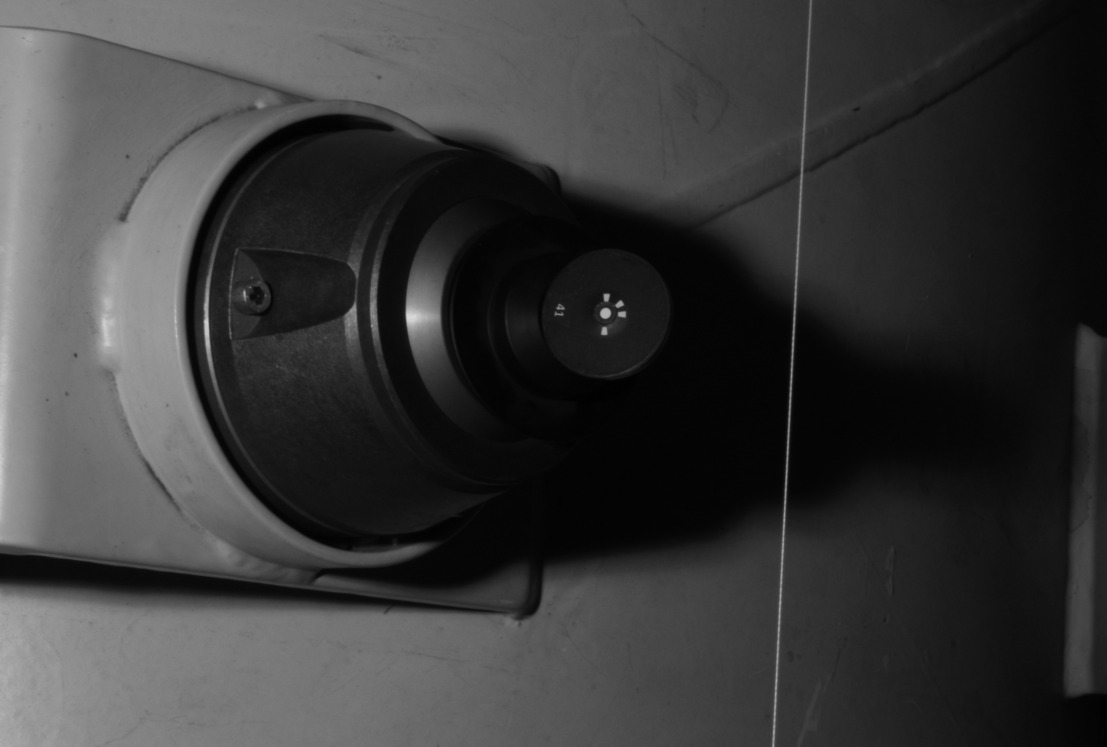
\includegraphics[width=4cm]{Methods/ImagesFils/ImagOri.jpg }
        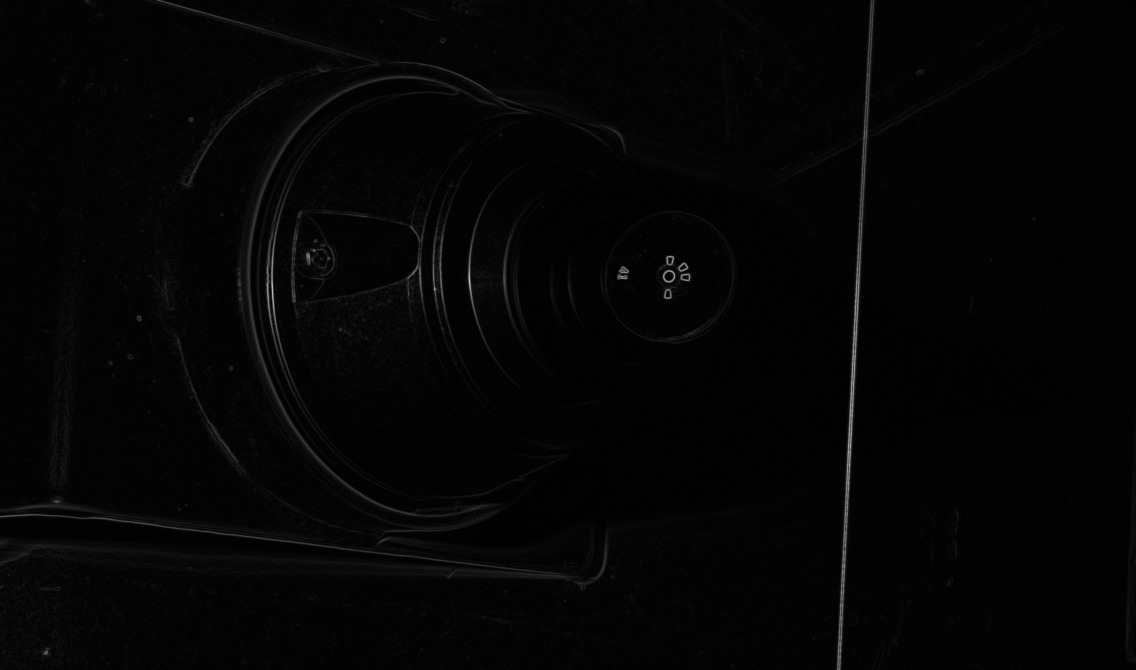
\includegraphics[width=4cm]{Methods/ImagesFils/GradInit.jpg }
        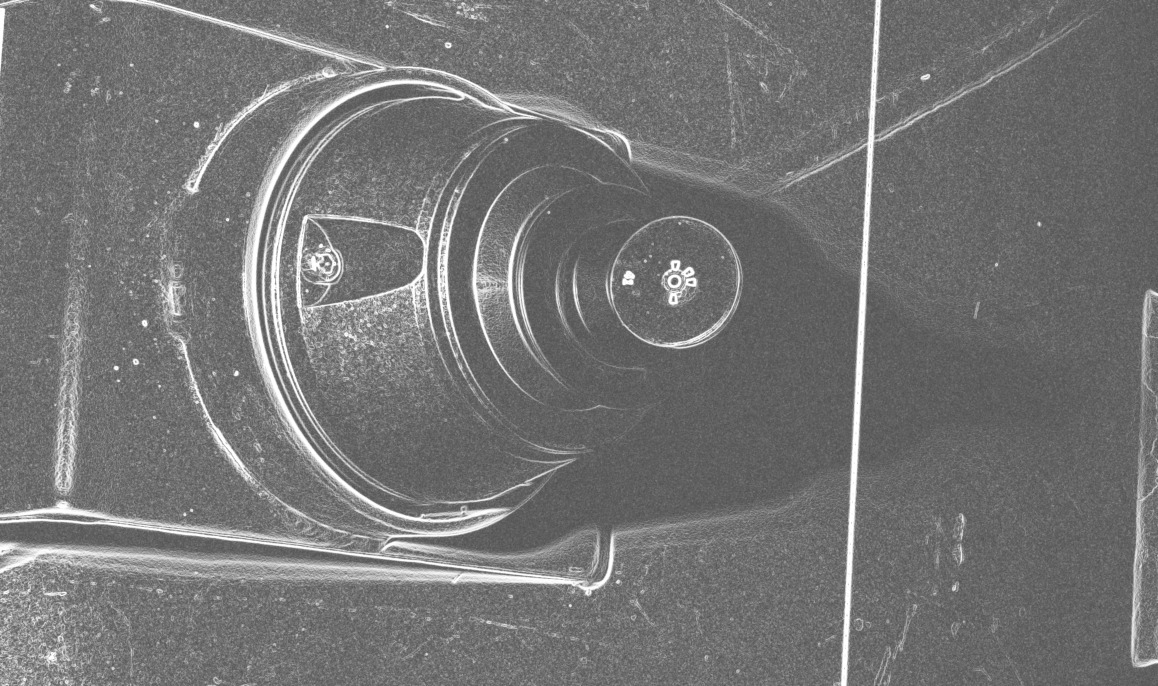
\includegraphics[width=4cm]{Methods/ImagesFils/GradNonLinear.jpg }
        \caption{An extract of image, the sobel gradient, non linear radiometric enhance of gradient}
\label{Fig:Line:Grad}
\end{figure}

%-----------------------------------------------------------------------

\subsection{Selection of local maxima of gradient}

\label{Line:LocMaxGrad}

Extracting the local maxima of the gradient in the direction of gradient is a very classical pre-processing
in computation of  edge detection.  But there is some precuation  to tack into account here because :

\begin{itemize}
   \item on want side we want to select point that are maxima on sufficiently large neighboorhoud
         to have an efficient pre-filter (the point selected will be used for hough transform which
         can be relatively long);

   \item on the other side, we must tacke into account that for each line we want to detect, there exist 
        a close anti-parallel line, that will have a module of gradient comparable; due to noise,
        sampling, background, this anti parallel line may eliminate the point.
\end{itemize}

To avoid elimination of many points by their macthing anti parallel line, we proceed this way,
illustrated by left schema of figure~\ref{Fig:Line:MaxLocGrad} :

\begin{itemize}
   \item let  $P$ be a pixel of image were gradient is $\vec G$

   \item  $\rho_0$ and $\rho_1$ be two thresholds, low and hig, of size of
          and $\theta$ be angular threshold
           (value  $\rho_0=1$, $\rho_1=8$ and $\theta=\frac{\pi}{2}$ are used in {\tt ExtractLine})

   \item  we define $N_1$  the neighbourhoud defined by point $Q$ with $\vec u = \overrightarrow{PQ}$ such
          that  $ < \rho_1$  and $ | \widehat{\vec G \vec{u}} | < \frac{\theta}{2}  $

   \item idem for $N_0$


   \item we define also $N_1^+$  by  $N_1^+ = \{Q \in N_1 / \vec u . \vec G >0\} $
          (and similarly $<0$ for $N_1^-$).
          \footnote{if the the wire is  black, instide of white, the definition
           of $N_1 ^-$ and $N_1 ^+$ are swapped}

\end{itemize}

Now, to select  a point as a local maxima of the gradient we require that the following condition are
all satisfied :

\begin{itemize}
    \item  $|\vec G(P)|  \gg  |\vec G(Q)|  \forall  Q \in N_0$ , in the  \emph{small} neighbourhood , there is no risk
           to meet the anti-parallel line;

    \item  $|\vec G(P)|  \gg  |\vec G(Q)|  \forall  Q \in N_1 ^-$ in the direction opoposed to gradient, there is
           no risk to meet the anti-parallel line 

            
    \item  $ (|\vec G(P)|  \gg  |\vec G(Q)|)  or (\vec G(P) . \vec G(Q) <0 )    \forall  Q \in N_1 ^+$

\end{itemize}

Where the relation  $ |\vec G(P)|  \gg  |\vec G(Q)| $ stands for :

\begin{itemize} 
     \item  $|\vec G(P)|  > |\vec G(Q)| $  
     \item or $(|\vec G(P)|  == |\vec G(Q)|) and (x_P >x_Q) $ 
     \item or $(|\vec G(P)|  = |\vec G(Q)|) and (x_P =x_Q)  and (y_P=y_Q)$
\end{itemize} 

This definition is made so, for mathematicall consitency,  $\gg$  is a strict order relation.
The result of this selection is illustrated on left image of  figure~\ref{Fig:Line:MaxLocGrad}.

\begin{figure}
\centering
        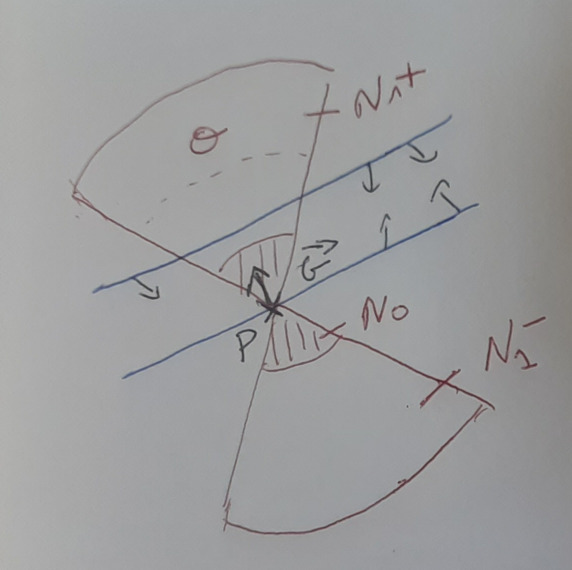
\includegraphics[width=6cm]{Methods/ImagesFils/NeighMaxLoc.jpg}
        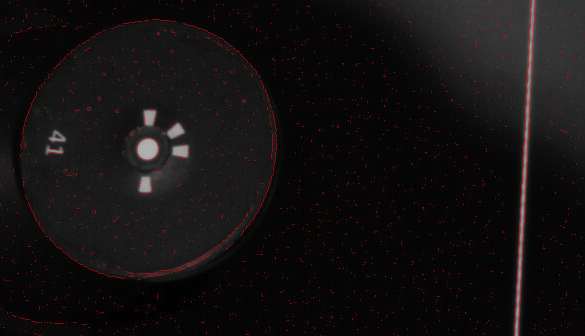
\includegraphics[width=6cm]{Methods/ImagesFils/MaxLocGrad.jpg}
        \caption{An extract of image, the sobel gradient, non linear radiometric enhance of gradient}
\label{Fig:Line:MaxLocGrad}
\end{figure}

On the tested images, with the used parameters, the proportion of pixels selected by this
procedure is less than $2\%$ of the initial set of pixels.


%-----------------------------------------------------------------------

\subsection{Refinement of local maxima}
\label{Ref:Grad:Loc:Max}

The previous selection return a set of pixels with integer coordinates, to have a better accuracy
their coordinates are then refined. The method used is the following , let:

\begin{itemize}
     \item  $\vec g =  \frac{\vec G}{|G|} $ be the unitary vector in direction of gradient;

     \item   $G_{1} = |\vec G(P+\vec g)|$ the norm of gradient at $1$ pixel distance in direction of gradient;
     \item   $G_{-1} = |\vec G(P-\vec g)|$  and $G_0 = |\vec G(P)|$
\end{itemize}

Consider now the parabol $\mathcal {P}$  such that  : $\mathcal {P}(-1) = G_{-1} $ , $\mathcal {P}(0) = G_{0} $ ,
$\mathcal {P}(1) = G_{1} $. Except in degenerate case, this $\mathcal {P}$ has a single extremum , note it $a$, we
then set  $P_r = P+ a\vec g $ , where $P_r$ is the refined point. On this simple bases, there is several
modification :

\begin{itemize}
    \item if we are in the degenerate case, or if the extremum is a minima we dont do anything;
    \item if $|a| > 1 $ we dont do anything;
    \item we make several iteration of this process ($2$ in the current code).
\end{itemize}

The corresponding code can be found in the method {\tt cImGradWithN<Type>::RefinePos}.


\TOIMPROVE{ maybe  try a metho that dont use gradient and its interpolation, like method computing directly
            the gradent in the interpolation, with a derivale interpolator like sinc of cubic }

%-----------------------------------------------------------------------
%-----------------------------------------------------------------------
%-----------------------------------------------------------------------

\section{Computation in hough space}

%-----------------------------------------------------------------------

\subsection{Notation and reminder of the hough transform}

Let $x,y$  be the set of  pixel of the image.  Let $D$ be a line parametrized
by $\rho, \theta$,  such that :

\begin{equation}
     x,y \in D(\rho,\theta)   \Leftrightarrow  x \cos (\theta) + y \sin (\theta) = \rho  \label{Line:EqRadon}
\end{equation}

The hough-transform is used here for counting for each lines 
the number of points through which it passes . It's very similar to radon
transform, it's somewhat just an inversion of  the process :

\begin{itemize}
    \item in radon transform, we parse all the possible line,i we sample the  line
          and count the sum of the image (function ) on the line;

    \item in hough transform we parse all the pixel, and for each pixel we
          sum the function in accumulator $H$  on all the lines that pass trough the point ,
          for this we use equation \ref{Line:EqRadon} to make the incrementation
          of equation \ref{Line:EqHough}.
         
\end{itemize}

\begin{algorithm}
\caption{Hough incrementation of $H$  for $x,y$ with value $I$}\label{alg:hough}
\begin{algorithmic}
\State $K_t \gets NbT$ \Comment{$ NbT$ : number of sampling in teta}
\While{$K_t \neq 0$}
    \State $\theta  \gets  \frac{2 K_t \pi}{NbT} $
    \State $\rho \gets  x \cos(\theta) + y \sin(\theta)  $  \Comment{This is a comment}
    \State $H(\theta,\rho) += I$
\EndWhile
\end{algorithmic}
\end{algorithm}

%-----------------------------------------------------------------------

\subsection{Oriented hough transform}

In general case, hough transform is equivalent to radon transform and relatively
slow, if the image has a size $N \times N$ , the computation time is in $N^3$.
What make hough very popular is that it can be very efficient in the case where
for the majority of point  we have $I(x,y) =0 $, because in this case we dont
need to enter in the loop~\ref{alg:hough}.
This is more a less what we do  with the computation of local maxmima in \ref{Line:LocMaxGrad},
instead of executing \ref{alg:hough} for all pixel, we do it for only the few \% of pixel
that were selected as local maxima.

By the way, there is more to do, because when we compute the gradient we have not only
its module but also its direction $\alpha$, so it is coherent to suppose that if
a straight line of  Hough/Radon-coordinate $\rho,\theta$ pass by this point we have $\theta \approx \alpha$.
Note, that doing that we consider \emph{oriented} line where direction are defined $\equiv 2 \pi$
and not single line defined  $\equiv \pi$; which is rather an advantage  if we want to
extract both each line and its antiparallel homologous they become distant in Hough/Radon space. 

So for each point, in  algoritm~\ref{alg:hough},
due to estimation $\alpha$ of $\theta$, we can reduce the initial
interval $[0,2\pi]$  to  $[\alpha-\delta,\alpha+\delta]$ where $\delta$ is  
the estimation of incertitude .  In command {\tt ExtractLine}, the default value
is empirically set to $\delta=0.1$, which seem safe enough and lead to an acceleration
of factor $30$ of hough transform.


The code corresponding to algorithm~\ref{alg:hough} can be found in method  :
\begin{itemize}
  \item {\tt void  cHoughTransform::Quick\_AccumulatePtAndDir(const cPt2dr \& aPt,tREAL8 aTetaC,tREAL8 aWeight); }
  \item {\tt void  cHoughTransform::Accurate\_AccumulatePtAndDir(const cPt2dr \& aPt,tREAL8 aTetaC,tREAL8 aWeight); }

  \item  once we have sampled the different value of $\theta$ the formula~\ref{Line:EqRadon} gives a real value
         of $\rho$, which does not fit exactly on a pixel of acccumularor, in quick version we simply round
         to nearest integer, while in second we split it using linear interpolation; by default  {\tt ExtractLine}
         uses quick version.
\end{itemize}

The figure~\ref{Fig:Line:Hough} represent the typical  result  we obtain at this step.

\begin{figure}
\centering
        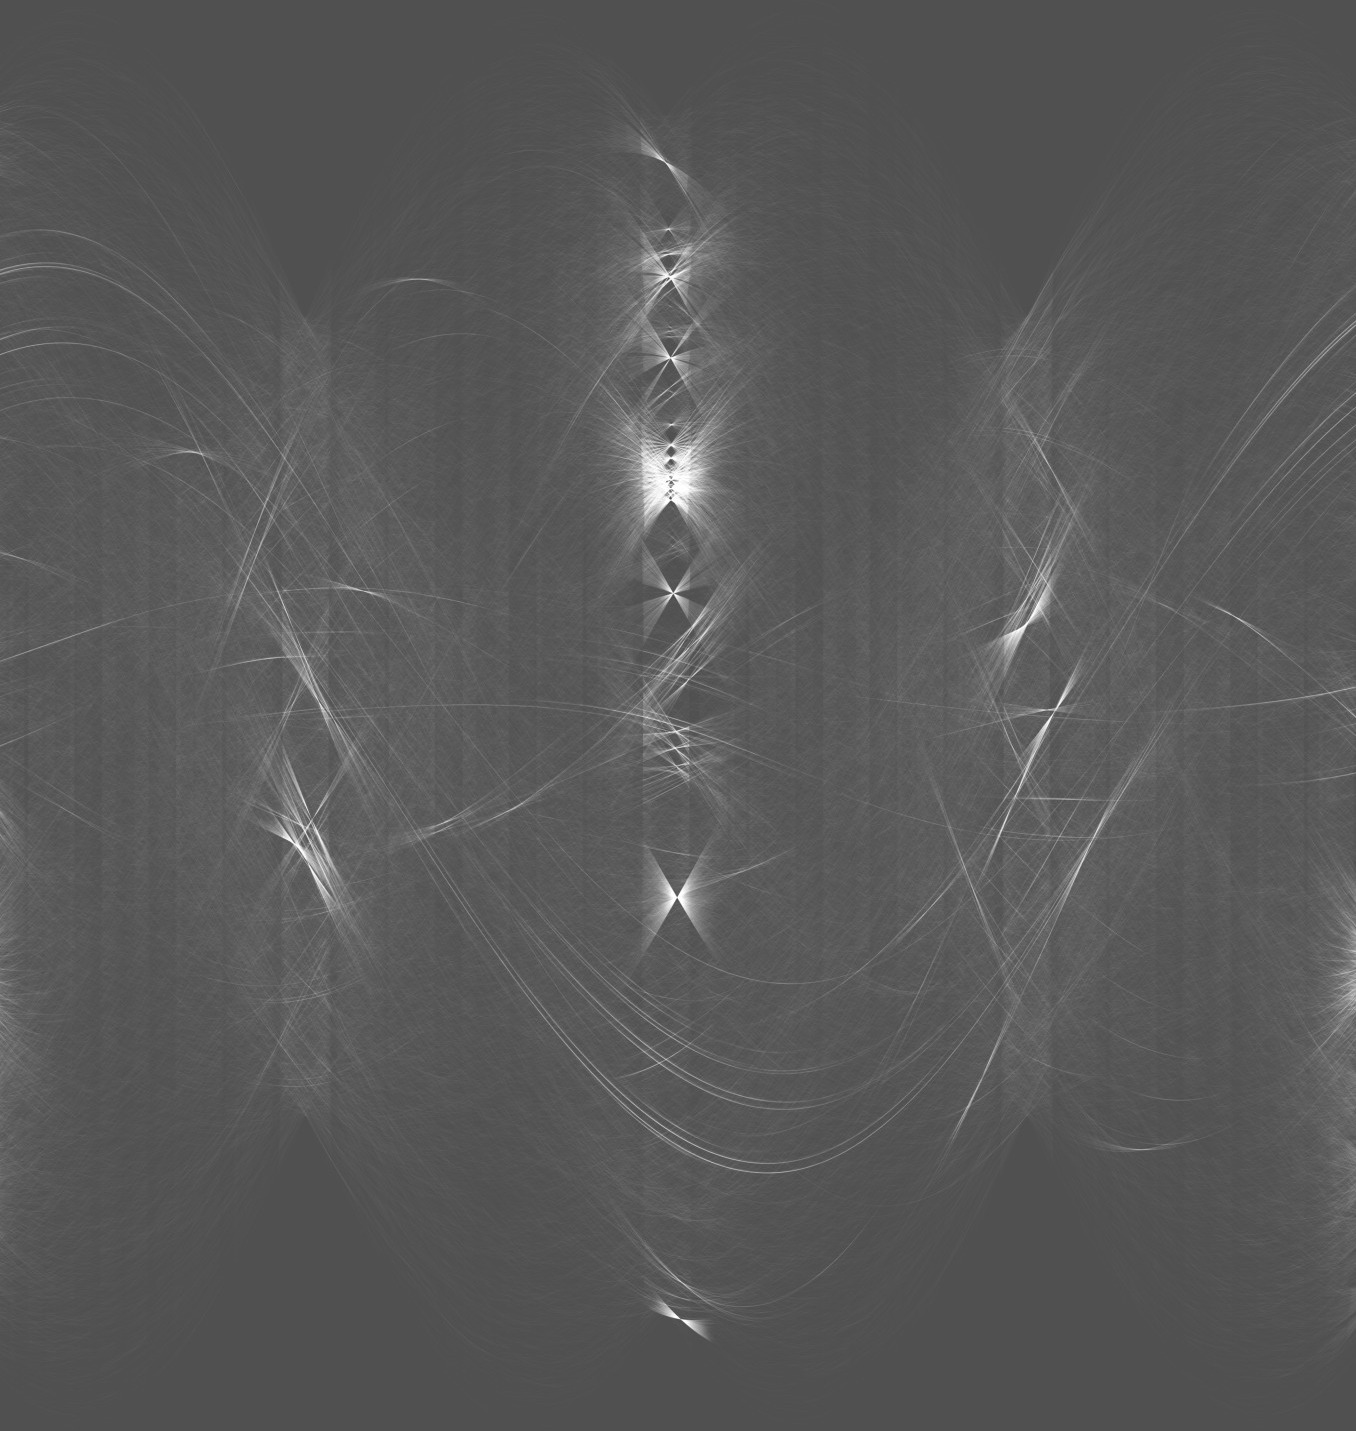
\includegraphics[width=8cm]{Methods/ImagesFils/FullHough.jpg}
        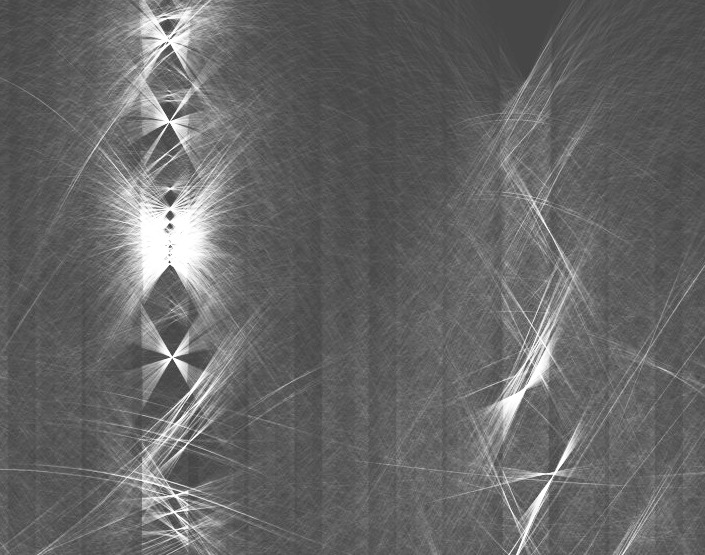
\includegraphics[width=8cm]{Methods/ImagesFils/Crop-Hough.jpg}
        \caption{Example of hough transform, and a crop on it}
\label{Fig:Line:Hough}
\end{figure}


%-----------------------------------------------------------------------

\subsection{Extraction of maxima of hough transform}

\label{Hough:Max:Loc}

The next step is to extract the "best" line candidate in hough space, 
this is done in  following steps :

\begin{itemize}
    \item  compute a threshold $Th$  taking into accound average $Avg_H$ and max $Max_H$ of hough accumulator,
           in current version $Th = \max (10*Avg, \frac{Max_H}{10})$
%    std::vector<cPt3dr> aVMaxLoc = mExtrL->Hough().ExtractLocalMax(10,5.0,10.0,0.1);
% std::vector<cPt3dr>  cHoughTransform::ExtractLocalMax(size_t aNbMax,tREAL8 aDist,tREAL8 aThrAvg,tREAL8 aThrMax) const
    \item  extract all the point for which $H(\rho,\theta) > Th$ and that are a local maxima in a 
           given neighbourhood, in current version of size of the neighbourhoud is $5$;

     \item once we  have selected the local maxima, we select if necessary the $K$  highest point, here $K=10$;

     \item finaly we refine the position to transform the integer value in real value, classically we compute
           the value in a neigboorhoud (here the $8$ neighboors), fit a quadratic functions on these values
           and extract  the maximal value.
\end{itemize}

This extraction is done in the method :

\begin{itemize}
   \item {\tt std::vector<cPt3dr>  cHoughTransform::ExtractLocalMax(size\_t aNbMax,tREAL8 aDist,tREAL8 aThrAvg,tREAL8 aThrMax) const;}

\end{itemize}


%-----------------------------------------------------------------------
%-----------------------------------------------------------------------
%-----------------------------------------------------------------------

\section{Back to image space computation}

%-----------------------------------------------------------------------

\subsection{Refine line in image space} 

\label{Line:Ref:ImSpace}

It is more accurate to use the initial pixel coordinates for extracting
the fine coordinate of each line. This is done using a weighted least-square fitting.
For each hough-point $\rho, \theta$ selected
(by~\ref{Hough:Max:Loc}) ,  we compute the line $D$ and do the following process :

\begin{itemize}
   \item  extract the local maxima of gradient (as in~\ref{Ref:Grad:Loc:Max}) that are
          at distance of $D$ inferior  to a given threshold  (here $2.0$ pixel), 
          and whose gradient is close enouh to normal of $D$ (here we use $\frac{\pi}{10}$);

    \item for each point $p_k$  at distance $d_k$ compute a weight $W_k=\frac{1}{1+\frac{d_k}{\sigma}^2}$,
          where $\sigma$ is the a priori estimation of variance (here we use $\sigma=0.2$);

     \item estimate by least squate the $D'$ minimizind $\sum_k W_k d(D',p_k)^2 $

     \item eventually iterate.
\end{itemize}


This refinement  is done in the method :

\begin{itemize}
   \item {\tt  void  cExtractLines<Type>::RefineLineInSpace(cHoughPS \& aHPS)} ;

\end{itemize}


%-----------------------------------------------------------------------

\subsection{Match anti parallele line}

Now we have a set of line that may be potentially the contour of a wire, to reconstruct 
the wire we must match the two anti parallel line that constitute the wire.  We say
that two oriented line match if :

\begin{itemize}
    \item  their anti parallel , with a given threshold (here we use $6e-4 rad$ ) 
    \item  the distance of the middle of each line to the other is in a given interval
           (here we use $[2.0,7.0]$,  maybe dangerous to have a too strict value)

    \item  their relative position (left/right, taking into account orientation) 
           is compatible with the fact that the line is white or black;
\end{itemize}

This match method is implemented in :

\begin{itemize}
   \item {\tt  bool cHoughPS::Match(const cHoughPS \& aPS2,bool IsLight,tREAL8 aMaxTeta,tREAL8 aDMin,tREAL8 aDMax) const;}
\end{itemize}

Now for each detected line, we compute, if any, its matched line : the line that comply with previous rule and
and is the closest.  Finnaly we select as valid pair the line for which we have a reciprocal match.
This is implemented in :

\begin{itemize}
   \item {\tt std::vector<std::pair<int,int>> cHoughPS::GetMatches(const std::vector<cHoughPS>\&  aVPS,bool IsLight,tREAL8 aMaxTeta,tREAL8 aDMin,tREAL8 aDMax);}
\end{itemize}



%-----------------------------------------------------------------------

\subsection{Central wire extraction and Quality evaluation}

For selected lines, we compute then the central wire, that contain a line (middle of two matched lines) and  a whidth.
Different quantities are computed to evaluate the quality of the wire, in the case where the line would contain
several lines that can generate false positive :


\begin{itemize}
   \item  sum of weight $SW$ of  match gradient point (as defined in \ref{Line:Ref:ImSpace})
   \item  parallelism of the two anti paralel line line;
   \item  homogeneity of radiometry measured in the center of the wire.
\end{itemize}

\TOIMPROVE{ Add the sigma from least square fitting, as additionnal criteria}

The criteria on homogeneity is based on the folowing expectation :

\begin{itemize}
   \item  the "real" wire being on the foreground is never interupted, and it radiometry should be
           smooth (the radiometric variation are due to the vignettage and flash)
   \item  the "false" wire are object, put on the magnet that are often interupted which create
          radiomatetric discontinuities (see the typical two profiles on  figure~\ref{Fig:Line:RadiomProfil}.)
\end{itemize}

\begin{figure}
\centering
        
\includegraphics[width=14cm]{Methods/ImagesFils/ProfilOK.jpg}
        
\includegraphics[width=14cm]{Methods/ImagesFils/ProfilNotOk.jpg}
        \caption{Two radiometric profil, one of a "true" wire, the other for a false positive}
\label{Fig:Line:RadiomProfil}
\end{figure}

The radiometric homogeneity if computed this way :

\begin{itemize}
   \item  a median filter is applied (size $3$) is applied,
          this low frequency filter aims at supressing the random noise,
   \item  then the total difference between the signal and convolution by a gaussian filter $\sum |I-I \circledast G| $ is computed
          to estimate the variations;
   \item  the  homogeneity is the total variation divide by the average (to have a measure
          invariant to global lighting).
\end{itemize}

This estimation of radiometric  homogeneity can be found in :

\begin{itemize}
   \item {\tt void  cParalLine::ComputeRadiomHomog(const cDataGenUnTypedIm<2> \& anIm,cPerspCamIntrCalib * aCalib,const std::string \& aNameFile)};

\end{itemize}

%-----------------------------------------------------------------------

\subsection{Selection of  \emph{best} lines}

We must now make a decision, ideally detect $1$ and only $1$ wire, but handle the case
were there is no wire, or multiple wire.


Firt if the list of candidate is not empty we consider the wire that maximize the sum of weight $SW$
defined bellow ( $\pm$ the one fitted by the maximum of points). All the other can be rejected if 
the best one is signficantly better, to see the rule used, examine the method

\begin{itemize}
   \item  {\tt bool cParalLine::RejectByComparison(const cParalLine \& aBetterOne) const;}
\end{itemize}


%-----------------------------------------------------------------------
%-----------------------------------------------------------------------
%-----------------------------------------------------------------------

\section{The \PPP command }

The command for line extraction is {\tt ExtractLine}. It takes $4$  mandatory parameters  in the following order :


\begin{itemize}
   \item  the set of images where the line must be extracted ;
   \item  a boolean indicate if the wire is white  (used when orientation of line is meaningfull like computing neighboorhouds
          or matching anti parallel line);
   \item  a folder indicating the location of an existing calibration  \footnote{it is planned to be able to use
          it w/o calibration using the key word {\tt NONE}, by the way it is still not fully working};
   \item  a folder where storing the results.
\end{itemize}

For example :

\begin{verbatim}
   MMVII ExtractLine  AllImFil.xml   true BA_311_C Fils 
   MMVII ExtractLine  (.*)_0158.tif  true BA_311_C Fils 
   MMVII ExtractLine  043_0158.tif   true BA_311_C Fils 
\end{verbatim}

For example with last command :

\begin{itemize}
    \item we will extract white line on image {\tt 043\_0158.tif};

    \item for distorsion correction we will look for intrisic calibration in 
          folder {\tt MMVII-PhgrProj/Ori/BA\_311\_/} ;

    \item the result will be stored in folder {\tt MMVII-PhgrProj/PointsMeasure/Fils};
\end{itemize}

The result will be stored in two way :

\begin{itemize}
    \item a xml file by image, that is used by \PPP ;
    \item a global file {\tt Lines.csv} that is generated for convenient use by external software.
\end{itemize}


%   -  -  -  -  -  -  -  -  -  -  -  -  -  -  -  -  -  -  -  -  -  -  -  -  -  -  -  -  -  -  -  -  -  -  -  -
% \subsubsection{AAA}









\include{Methods/AimeDesc}
\include{Methods/TiePoints}
\include{Methods/Vrac}

%###########################################################################################################
%###########################################################################################################
%---------------------------------------------- PROGRAMMER DOC --------------------------------------------
%###########################################################################################################
%###########################################################################################################

\part{Programmer's doc}

\include{Programmer/ProgrammingStyle}

\include{Programmer/Serialization}



\chapter{Use of non linear optimization in MMVII}

\label{Chap:NLO}

This chapter is targeted for programmer that will increase MMVII, it mainly describe classes
interfaces in headers and a detailled example of using this classes in a cpp file.
 It's not useful for advanced users; on the other hand, for programmer who will maintain the core of MMVII, 
more detailled documentation will have to be written.

At this step, the chapter has no theoretical presentation, it assumes that the reader is familliar
with least square, linearization, Gauss-Newton, Schur complement\dots


%---------------------------------------------
%---------------------------------------------
%---------------------------------------------

\section{Introduction}

%---------------------------------------------

\subsection{Quick formalization}

This chapter presents the classes used in MMVII for non linear optimisation using some Gauss-Newton methods. 
By non linear optimisation, we mean minimize $F(X)$ with :

\begin{equation}
      F(X) = \sum_{j=1,M} w_j f_j(X)^2  \;  X \in \RR^n  \label{EqNLOInit}
\end{equation}

The assumpution on the problem are classical :

\begin{itemize}
   \item we have an initial guess $X_0$ on $X_{min}$  , this guess is sufficiently 
         good for the local minimal we will (hopefully) find to be a global minimum;

   \item the function $f_j$ are differentiable (some weaker hypothesi are also possible)

\end{itemize}

The service offered by MMVII are typically those a Gauss-Newton iterations : 
use current estimation $\tilde X$ of $X_{min}$ for linearizing the $f_j$ and 
solve equation $\ref{EqNLOInit}$ by least square methods.

%---------------------------------------------

\subsection{2d-Triangularton problem in general}

We will illustrate the presentation by a detailled example that is used for testing correctness of the
implementation. Also relatively basic, this example should be sufficient for a first 
understanding and utilisation of the MMVII classes. The $2d$-triangulation problem we treat
here is the following :

\begin{itemize}
    \item we have a set of points $P_1 \dots P_n$ , each $P_k$ belongs to $\RR^2$;

    \item we do not know the exact values of $P_k$ but we have an initial estimation  $P^0_k$
          which is not too bad, whatever it means;

    \item for a certain number of pair $P_i,P_j$ we have a measurement of the distance $d_{ij}$ between
          $P_i$ and $P_j$,
\end{itemize}

The triangulation problem  consist to use the measurement of distances for recovering the unknown
value on $P_i$.  Let $M$ be the  number of pair for which we have measurement 
Let $X \in \RR^{2n} = \{P_1 \dots P_n\}$ be the unkown vector,
we typically want to find $X$ that minmize $D$ defined by :

\begin{equation}
      D(X) = \sum_{j=1,M} (d_{ij} -d(P_i-P_j))^2  \label{EqConsDist}
\end{equation}


Of course as the fonction $D$ is invariant to any isometry of the plane, the minimization
of $D$ would be an ill-posed problem, as for any set of points, its image by a global rotation
will give the same value. To ensure uniqueness of the solution  will force the value of
a certain number of coordinates.

%---------------------------------------------

\subsection{2d-Triangularion in this example}

As we want the example to be as simple as possible, and also we want to use it for checking
the correctness, the data will be different from a real one , the figure~\ref{fig:NetFull} illustrates 
this network:

\begin{itemize}
    \item the "real" value of points will be positionned on a regular grid, typically we
           will have $(2*N+1)^2$ points, each point having integers corrdinate 
           $(x,y) \in [-N,N]^2$

    \item we will have measure between pair of point that  are $8$-neighoor i.e
          $max(|x-x'|,|y-y'|)\leq 1 $ , this is sufficient for the solution to be unique
          up a rotation ;

    \item in real life  $d_{ij}$ would be noisy, but here in this simulation example we
          use the exact value because, to check correctness of the library, we want to check 
          that we are able to recover the exact values of coordinates.
\end{itemize}

Regarding the arbirtrary constraint we will keep it as simple as possible, so 
considering the two points of the grid  $A=(0,0)$ and $B=(0,1)$ , we will add the following
constraint to the minimization :

\begin{equation}
      x_A=0  \;  y_A=0  \;  x_B=0 \label{Eq:FixVarAB}
\end{equation}

The two first constraint freeze the solution in translation, while the last one freeze the rotation.


\begin{figure}
\centering
\includegraphics[width=12cm]{Methods/Images/T90-NetFull.JPG}\caption{Network, case w/o schur}\label{fig:NetFull}
\end{figure}



%---------------------------------------------

\subsection{Use of schur complement}

Schur complement is an efficient way to treat the case where there is a subset of variable that 
occurs in \ref{EqNLOInit}, but for which we are not specially interested in exact values ,
 however but we want to take them into account rigourously in 
the computation of the others. Once we know
\emph{all} the equations where such  subset of variable is involved, schur
complement offer a way to eliminate them without altering the value of the minimum.

A typical case is in bundle adjsutment, when we are interested only to the value
of camera parameters and not by the value of $3d$ points involved by the projection
equation. In this case, suppose we will typically  have $1000$ camera and $1000000$ points,
doing schur elimination can reduce the system from $3000000$ unkwnon to $6000$.



In our toy example, the schur complement will be purely artificial. When the
{\tt WithSchur}  option is activated, the network is modified in the following
way, the figure~\ref{fig:NetSchur} illustrates 

\begin{itemize}
    \item all the points on the line $x=1$ are considered as temporay variable,
          i.e variable that we want to eliminate, we will not  know their value at the
          end of the computation; 

    \item there will be no conexion between points of line $x=1$ (for example $(1,2)$
          and $(1,3)$ that were connected in previous case are non longer
\end{itemize}

\begin{figure}
\centering
\includegraphics[width=12cm]{Methods/Images/T90-NetSchur.JPG}\caption{Network, case with schur}\label{fig:NetSchur}
\end{figure}

%---------------------------------------------

\subsection{Files of MMVII involved}

We make a quick enumeration of files of MMVII that are to access for understanding :

\begin{itemize}
    \item {\tt include/MMVII\_SysSurR.h} contains the declaration of the class relatives to
          non linear optimisation, from the user point of view the main class
          is {\tt  cResolSysNonLinear};

    \item files on folder {\tt src/TutoBenchTrianguRSNL/} contain the code for the $2d$-triangulation
          example;

    \item {\tt src/SymbDerGen/Formulas\_Geom2D.h } and {\tt src/SymbDerGen/GenerateCodes.cpp } 
          contains the code for generating the automatic differentiation 

    \item {\tt src/GeneratedCodes/CodeGen\_cDist2DConsVal.cpp } contains the code for 
          generating the automatic differentiation , also it is theoretically not necessary 
          to see it for using it, it's no harm to be curious and not use it as a black box;
          by the way in real case use, it will not be necessary to look at the code that you
          will generate.
\end{itemize}

%---------------------------------------------
%---------------------------------------------
%---------------------------------------------

\section{Computing functions and their derivatives}
\label{Compute:Deriv:SysNL}

%---------------------------------------------
\subsection{Motivation}

For Gauss Newton iteration, in equation \ref{EqNLOInit}, we will need to compute not only
the $f_j$ but also all its partial derivative $\frac{\partial f_j}{\partial x_i}$
relatively to all variable $x_i$ used in $f_j$.  There are many way to do it,
and to be honest  all have  pro and cons:

\begin{itemize}
    \item numerical derivative are the most simple, but they are slow, and can be unacurrate
          when the "small" value are not correctly choosen;

    \item hand crafted derivative are accurate and can be fast, however they can be complicated
          to write for real case formula (like arrise in bundled adjustement) and can be
          a nightmare to maintain when a "small" change occurs in the formulas;

    \item jet derivative, like used it Ceres, are almost as simple to use as numericall, once
          you have the library,  and much faster and accurate as numerical ones; they are much
          easier to use and maintain as  hand crafted ones, but can be also slower than
          handcrafted;

    \item symbolic derivative and code generation, can be a bit more complicated to use
          than jet, especially the first time; however after  this quick learning step
          they are as easy as jets to use,  easy to maintain and, in some case, much
          faster.
\end{itemize}

The solution implemenented in MMVII in based on symbolic derivative with code generation.
This choice was made because it is believed that programmer that will goes into the
core of MMVII have rather high requirement in code efficiency and are ready to pay a
small learning steps.

%---------------------------------------------
%\section{Generating the code}

          %  - - - - - - - - - - - - - - - - - - - 

\subsection{class for specifying the formulas}

\label{Class:Specif:Formulas}

In this  example, we have only one formula we need to compute and derivate, it's
the formula of equation~\ref{EqConsDist}.  First introduce a bit of MMVII's jargon  :

\begin{itemize}
   \item in this formula we have two different kind of variables the $P_i$ and $P_j$
         and the $d_{ij}$;
         
   \item for the $P_i$ themselves we have no direct observation , we only have initial value,
         and our target is precisely to compute their values; they will be named {\tt unkowns};

   \item for the $d_{ij}$ we know their values (it could be with some uncertaincy, but that'
         another story) and dont try to compute it, they will be name {\tt observations}.
\end{itemize}

The class {\tt cDist2DConservation} in file  {\tt src/SymbDerGen/Formulas\_Geom2D.h } contains
all the information that are required for generating code. It must define $5$ members :

\begin{itemize}
   \item a contructor, that does nothing for such a basic example

   \item a method {\tt VNamesUnknowns} that return the vector of names of unkown ,
         here we have $2$ points and $2$ coordinates $x,y$ for each points so the
         vector has a length of $4$;  the names will be used for code generation;

   \item a method {\tt VNamesObs} that return the vector of names of observations ,
         here we have a single observation which is the targeted distance between 
         $P_1$ and $P_2$;  the names will be used for code generation;

   \item a method {\tt FormulaName}  that return the name of the formula itself,
         the method will be used for the name of class and files containing the generated
          code;

   \item a method {\tt formula}  this is the core of the class, this method
         take as input a vector of unknown and a vector of observation and return
         a vector that is the result of the  computation  (typically a residual
         when used in context of gauss newton);  the type of {\tt tUk} of the
         i/o vectors and of temporary variable, is not very important at this step,
         it's suffice to know that it is a type on which most current mathematicall
         operation are defined (and can be completed when missing), they represent
         mathematical formula as symbolic tree; see \RefFantome for detailled
         explanation on the type {\tt cFormula<Type>} defined in 

\end{itemize}

Regarding the $3$ methods that  return names, as they are used as \CPP identifier
its important that they contains only valid character (alpha numeric and {\tt\_} ,
no {\tt + - ...}),  also it's important that  inside a vector they are unique.
Apart of that, their exact name is unimportant, but giving names semantically
meaningful is useful if a human want to read the generated code (something we
generally dont do, but something we will do here).

\begin{equation}
      D(X) = \sum_{j=1,M} (\frac{d(P_i-P_j)}{d_{ij}} - 1)^2  \label{EqConsDistHom}
\end{equation}

Regarding the method  {\tt formula}, it's here a direct implementation 
of residual used in  equation~\ref{EqConsDistHom}, which
is non dimensionnal variant of equation~\ref{EqConsDist}. Some comment :

\begin{itemize}
   \item we make an intensive use of the {\tt auto} type specification which
         is convenient here;

   \item the less intuitive part is probably {\tt  CreateCste(1.0,x1);},  in fact
         when we need to create a constant  we must indicate the type of symbolic
         formula to the constant is create with adequate type, the {\tt x1} parameter
         is just used to indicate the type in the template function {\tt CreateCste},
         putting {\tt x2}, {\tt y1} or any other would have exactly the same effect;

   \item the function return a vector of formula, which here is of size $1$, and not
         single value, because in general, when we want to compute several values (like
         $x$ and $y$ residual in BA)  its more efficient and convenient to group 
         a multiple residual in a single formula that generating different formulas;
   \item below this function, there is another version which is commented. It's showing
         how to use {\tt SymbPrint()}, {\tt SymbPrintDer()}, {\tt SymbComment()} and 
         {\tt SymbCommentDer()} to document the generated code or to output (print) 
         values of expressions or parts of expression in the formula.
   \begin{itemize}
         \item {\tt SymbComment(expr, comment)} will place {\tt comment} as a comment
               on the line in the generated code where a tempory variable will be assigned
               the value of expr.
         \item {\tt SymbCommentDer(expr, k, comment)} will place {\tt comment} as a comment
               on the line in the generated code where a tempory variable will be assigned 
               the value of the derivative of expr with respect to the kth unknown.
         \item {\tt SymbPrint(expr, mesg)} will generate code to display at runtime
               "[i] mesg =  (value of expr)", i being the current iteration of the loop
               when multiple values are calculated simultaneously.
         \item {\tt SymbPrintDer(expr, k, mesg)} will generate code to display at runtime
               "[i] mesg = (value of derivative)", derivative being the derivative
               of expr with respect to the kth Unknown.
         \item to enable the output of this value, SetDebugEnabled(true) must be called
                before on the calculator. See \ref{CreateCalc}
   \end{itemize}
        With this (commented) example formula, the generated code would look like this:
        \begin{lstlisting}
<...>
double F31_ = (F30_ - 1);  // f
double F28_ = (F27_ / F14_);  // d(|v|)/d(p2.y)
double F18_ = (F17_ / F14_);  // d(|v|)/d(p1.x)
double F33_ = (D * F18_);
double F39_ = (D * F28_);
double F34_ = (F33_ / F32_);  // d(f)/d(p1.x)
double F40_ = (F39_ / F32_);  // d(f)/d(p2.y)
if (IsDebugEnabled()) {
  MMVII::StdOut()<< "[" << aK << "]  Vx=" << F9_ << std::endl;
  MMVII::StdOut()<< "[" << aK << "]  Vy=" << F8_ << std::endl;
  MMVII::StdOut()<< "[" << aK << "]  Dist2DConst=" << F31_ << std::endl;
  MMVII::StdOut()<< "[" << aK << "]  d(dist2DConst)/d(p1.x)=" << F34_ << std::endl;
  MMVII::StdOut()<< "[" << aK << "]  d(Dist2DConst)/d(p2.y)=" << F40_ << std::endl;
}
<...>
        \end{lstlisting}
\end{itemize}

As a slightly more complex example, the reader can investigate example {\tt cRatioDist2DConservation}
in the same file. This example correspond to the case what we want to preserve is not the distances
but the angles or ratio of distance. For each triangle $P1,P2,P3$, we have the initial 
distance $D_{i,j}$ as observation and  we write :

\begin{equation}
      \frac{d(P_i,P_j)}{D_{ij}} - \frac{d(P_i,P_k)}{D_{ik}} = 0 \label{EqRatioDist}
\end{equation}

In this cas we have $3$ equation and the function has $3$  values corresponding to the
$3$ possible combination of  equation~\ref{EqRatioDist}.

          %  - - - - - - - - - - - - - - - - - - - 

\subsection{Generating the code}

Once the class {\tt cDist2DConservation} has been created, the things to do for generating the
code is quite simple :

\begin{itemize}
    \item   add in file  {\tt GenerateCodes.cpp } a call to   the method {\tt GenCodesFormula}
            with an object of type {\tt cDist2DConservation}, note that we call it twice,
            the second boolean parameter indicating if we want to  compute the derivate;
            in fact sometime we will be interested only by the function and will not want
            to pay the price for the derivate;


    \item   compile with {\tt make}, execute a call to {\tt MMVII} command {\tt GenCodeSymDer},
            and compile again.
\end{itemize}


Also it's generally not necessary, we invite here the curious reader to give a look
at generated code.  All the such codes are located in {\tt src/GeneratedCodes/} ,
and here in the files  {\tt CodeGen\_cDist2DConsVal.cpp}, w/o derivative, and 
{\tt CodeGen\_cDist2DConsVDer.cpp}, with derivatives, the declaration of the classes
are in corresponding header file ({\tt CodeGen\_cDist2DConsVal.h} \dots). 
Note that the name used for file ans classes come from the result of {\tt FormulaName}.

Lets make a quick comment on {\tt CodeGen\_cDist2DConsVDer.cpp} :

\begin{itemize}
  \item  the computation is made in a loop {\tt for (size\_t aK=0;....)}, this 
         allow a paralelization of the code when high performance computation is
         required;

  \item  the name used for unkowns and observation can be recoginzed as local
         variable at the begining of the loop;

  \item  after the code is a very monotonous code with basic instructions as
         {\tt Fx = Fy op Fz;}  or {\tt Fx=Op(Fy);}  ,  this is not the way
         human would write code ...  however it is not made to be read and you may
         think of it as "high level assembleur code";

  \item  by the way the code is relatively optmized to avoid multiple redundant computation,
         for example you can see that formula {\tt F8}  that represent {\tt y1-y2} is computed
         once and used three time;

  \item  the result of one iteration contain $5$ value here, because we have the value of the function
         itself and the value of the derivative relative to the $4$ variable ($x$ and $y$ of
         $P_1$ and $P_2$) ;  

  \item  there is a high level interface for extracting independantly value and derivatives,
         but we will not need it here, as everything will be encapsulated in the main 
         class {\tt cResolSysNonLinear};

  \item  give a look at file {\tt CodeGen\_cRatioDist2DConsVDer.cpp}, in this case we have $21$
         values ; $21 = 3 * (1 + 3*2)$ , the ratio return a vector of $3$ values, and
         for each value we compute the value itself and its derivatives relative to the $6$
         variable ($x,y$ for $3$ points), again there is a high level interface for extracting
         these values.
\end{itemize}

          %  - - - - - - - - - - - - - - - - - - - 

\subsection{Creating the object}

\label{CreateCalc}

For computig the value and derivative of {\tt cDist2DConservation} in our \CPP program,
 a possible and classical way is to include the file declaring the class
(i.e. {\tt CodeGen\_cDist2DConsVal.h}) and explicitely create a {\tt cDist2DConsVDer}.

However the optimizer is done to work with any object deriving from the abstract mother
class of all object resulting from code generation :  {\tt cCompiledCalculator<double>};
so the optimizer only manipulate pointers on such class and the exact class is not used.
There is a function for creating an object from its name, and we create an allocator
from this name with the function {\tt  EqConsDist(bool WithDerive,int aSzBuf)}.

The definition in {\tt GenerateCodes.cpp }  is pretty basic :

\begin{lstlisting}
cCalculator<double> * EqConsDist(bool WithDerive,int aSzBuf)
{
    return cName2Calc<double>::CalcFromName(NameFormula(cDist2DConservation(),WithDerive),aSzBuf);
}
\end{lstlisting}


And the declaration in a header file (here {\tt MMVII\_PhgrDist.h} ) :


\begin{lstlisting}
NS_SymbolicDerivative::cCalculator<double> * EqConsDist(bool WithDerive,int aSzBuf);
\end{lstlisting}

Now from the user side, the only thing we need to do is calling  {\tt EqConsDist}. This
correspond in file {\tt BenchResolSysNonLinear.cpp}  to line:


\begin{lstlisting}
     mCalcD =  EqConsDist(true,1);
\end{lstlisting}

If we want to display values specified with {\tt SymbPrint()/SymbPrintDer()} during calculus of mCalcD, we have to enable it:

\begin{lstlisting}
     mCalcD->SetDebugEnabled(true);
\end{lstlisting}

%---------------------------------------------
%---------------------------------------------
%---------------------------------------------

\section{Non linear system}

This section was written assuming that the user explicitely controls the numbering of all
the variable because this was the way it was done at the begining. Meanwhile, a mecanism
described in~\ref{SecAutoUkAlloc} has been added to facilitate this automatic numbering.
By the way the explicit numbering is still accessible, because it is believed that the
two mecanisms are useful.

\subsection{Introduction}

The class for solving  non linear system is the template class 
{\tt  cResolSysNonLinear<Type>}. This class provides an easy interface
for computing fonctions and their derivatives (via object resulting from code generation)
and weighted least squares in the aim of solving non linear systems.

The template of the class refers to the way linearized equation are store and solved.
Probably {\tt tREAL8=double}  would be a good default value, while {\tt tREAL16}
could be used when high accuracy is required.

The main operations that can be done with such solver are:

\UNCLEAR
\begin{itemize}
   \item create a solver with initial values of the unknowns and parameters for
          specifying the adjoint least square solver; 

   \item add directly  an equation on subset of unkowns \emph{w/o} temporary unknowns;

   \item add  an equation with a subset of unkowns \emph{with} temporary unknowns  to
         a structure that accumulate them;  then  add this structure to the solver;

   \item add equation fixing a given variable;

   \item acces to current solution;

   \item compute the next current solution and reinitialize the solver.

\end{itemize}


          %  - - - - - - - - - - - - - - - - - - - 

\subsection{Least square solving and constructor}

In {\tt src/TutoBenchTrianguRSNL/cMainNetwork.cpp} the call to these constructors can be found
after tags {\tt  BASIC:CONSTRUCTOR} and {\tt LEASTSQ:CONSTRUCTOR}.
The dense vector is created from a standard vector.\UNCLEAR

In {\tt MMVII} the core calculation of matrix algebra is realized
by eigen library. The services offered by {\tt MMVII} is essentially
an interface for storing data and for a more homegeneous integration
in {\tt MMVII} "philosophy".

In {\tt MMVII} there is several ways to handle least squares systems, each
one correspond to a value of enumeration {\bf \tt eModeSSR} :

\begin{enumerate}

    \item{\bf \tt eSSR\_LsqDense :}
          uses dense matrix for storing the normal matrix; for system not so spare,
          or for small systems, this is the most efficient way; typically if you have
          (many) thousands of limited size systems, this is the mode you must use; solving
          is made by calling \emph{"ldlt"} method of eigen (i.e. Robust Cholesky 
          decomposition of a matrix with pivoting); this classes use schur-complement
          for handling temporay unknowns;

    \item {\bf \tt eSSR\_LsqNormSparse :}
          uses sparse matrix for storing the normal matrix; this is probably the most
          general way and the most efficient in time and storage for most cases in 
          photogrammetry involving many pose estimations. Its
          drawback is that using normal equations increase the conditioning of the
          system, the potential problem increasing with number of unknowns; 
          solving is made calling  {\tt SimplicialCholesky} decomposition of eigen;

    \item {\bf \tt eSSR\_LsqSparseGC :}
          uses sparse representation that memorize all the individual obsertions;
          \emph{do not} use normal equations, the solving is made using
          {\tt LeastSquaresConjugateGradient} decomposition of eigen;
          \emph{do not} use Schur complement for temporary unknowns, they
          are processed like the other unknowns; according to eigen documentation
          this method is the more robust for poorly conditioned systems
          compared to {\bf \tt eSSR\_LsqNormSparse}, for big
          sparse system with a high proportion of temporary unknowns, 
          it's certainly less memory  efficient and it's probably
          less CPU-efficient (but intensive test remain to be done);

\end{enumerate}

The basic constructor takes an enum value as parameter to specify
the least square solver and an initial value:

\begin{lstlisting}
       cResolSysNonLinear(eModeSSR,const tDVect & aInitSol);
\end{lstlisting}


It is also possible to create a solver with an explicit least square solver.
This is usefull especially with {\bf \tt eSSR\_LsqNormSparse} because the memory
allocation (still in construction) is more complex and may require more parametrisation
from the user.  \UNCLEAR



          %  - - - - - - - - - - - - - - - - - - - 

\subsection{Adding a basic equation}

\label{AddBasicEq}

The tag  {\tt  BASIC:CALC} in {\tt BenchResolSysNonLinear.cpp} contain an example of such use.
The method for adding an observation is named {\tt CalcAndAddObs} :

\begin{lstlisting}
    void   CalcAndAddObs(tCalc * aCalc,const tVectInd & aVI,const tStdVect& aVObs,const tResidualW & aWeighter= tResidualW());
\end{lstlisting}

The $4$ parameters are :

\begin{itemize}
   \item {\tt aCalc} is a calculator as described in~\ref{CreateCalc};

   \item {\tt aVI} is a std::vector of  int that contains the index of unknowns used;

   \item {\tt aVObs} is a std::vector of  {\tt double} that contains the observation;

   \item {\tt aWeighter} is an object used for computing the weight of the observation, 
         the default value  associate a constant weight $1$, we will not discuss more 
         this parameter at this step.

\end{itemize}

What is done is what can be expected :

\begin{enumerate}
   \item  use  vector {\tt aVI} and {\tt aVObs}  to fill the parameters
          of the functor {\tt aCalc}; for {\tt VI} the index are used read the 
          values of the current unknown

   \item  execute the computation of {\tt aCalc} , that must  have been created
          with the {\tt WithDer} option at {\tt true};

   \item  use the result of differentiation and the weighting computed by {\tt aWeighter}
          to add a linearized equation in the least square system.
\end{enumerate}


          %  - - - - - - - - - - - - - - - - - - - 

\subsection{Adding with schur complement}

The tag  {\tt  SCHUR:CALC} in {\tt BenchResolSysNonLinear.cpp} contain an example of such use.
Adding equation with temporary variables, is slightly more complex, as the elimination
can only be done once we have all the equations involving a given subset of unknowns.
So the computation is done in $2$ steps : (1) create a structure, give at this initialisation
step  the current values of unkonws (2) accumulation in a structure 
with {\tt AddEq2Subst}, (3) using this structure
for adding the equation on unknowns after having done the elimination of temporary unknowns with
{\tt  AddObsWithTmpUK}

The structure is {\tt cSetIORSNL\_SameTmp<Type>}, the method for accumulating 
equation has the signature :

\begin{lstlisting}
    void  AddEq2Subst (tSetIO_ST & aSetIO,tCalc *,const tVectInd &,
                       const tStdVect& aVObs,const tResidualW & aWeighter= tResidualW());
\end{lstlisting}

In this method {\tt aVObs} and {\tt aWeighter} are identic to the equivalent in
{\tt CalcAndAddObs}. For the others :

\begin{enumerate}
   \item the first one {\tt cSetIORSNL\_SameTmp<Type>}, is the accumulating structure, it
	   constructor takes current values of temporaries;

   \item  the vector {\tt aVI} contains the  unknown and temporary unkown,  
	   conventionnaly the numbering of unknown is made with negative numbers starting from
           $-1$ to distinguish them from standard unknown, in this example they are $-1$ and $-2$,
           standard unknown are processed as before; 
         s  ee {\tt aVIndMixt} after tag {\tt SCHUR:CALC}

   \item  the vector {\tt aVTmp} contains the  values of temporary unknowns;
\end{enumerate}

Once the equation have been accumulated, it is sufficient to call {\tt AddObsWithTmpUK}
with the structure as parameter.

          %  - - - - - - - - - - - - - - - - - - - 
          %  - - - - - - - - - - - - - - - - - - - 
          %  - - - - - - - - - - - - - - - - - - - 

\subsection{Equation fixing a variable}

          %  - - - - - - - - - - - - - - - - - - - 
\subsubsection{Weigthed version for standard variables}

\label{WeightedFixVar}
The tag  {\tt  EQ:FIXVAR} in {\tt BenchResolSysNonLinear.cpp} contain an example .

It currently happen that the solution we compute is undetermined
up to  certain transformation.  If we do nothing, the least square
system will be not inversible and this will create problems.
A current way  to overcome this difficulty is to fix a set
of arbitrary variables.  In our case, as said in~\ref{Eq:FixVarAB}, 
we fix arbirtrarily $x_A,y_A,x_B$.  

The method {\tt AddEqFixVar} can be used for that, it takes $3$ parameters :
the number $k$ of the var, the value $V$ we want to assign, and the weight $w$
of the equation.  It simply add the following term  to the minimization :

\begin{equation}
      w (X_k -V)^2   
\end{equation}

The variant {\tt AddEqFixCurVar} fix the value of $x_k$ to its current value.

          %  - - - - - - - - - - - - - - - - - - - 

\subsubsection{Rigid fixing of a variable}

Sometime, we want to fix rigidly a variable to a given value.  Doing it with
a very high weight (almost "infinite") using method of~\ref{WeightedFixVar} would not be very 
good idea in general because the notion of very high weight is dependant of the context
and of the "dynamic" of the variable, and setting it to a universally  high value would lead to numerical 
instability.

In this case, the {\tt SetFrozenVar} familly must be used. The way it works is  totally
different of {\tt AddEqFixVar} and is the following :

\begin{itemize}
    \item {\tt MMVII} keep memory of all variable that have been frozen ;
    \item each time a linearized equation is added $\sum a_k X_k = B $ , for
             each $k$ where the variable $X_k$ is frozen to $F_k$ , $a_k$ is set to $0$ and $B$
             is set to $B - a_k F_k$;

    \item   also at the end (before solving) we had the equation $X_k=F_k$ with a weight of $1$
            for each frozen variable.
\end{itemize}

To have a correct behaviour of this "interception" mecanism it is required that all the frozen variable
are known before any equation is added. This constraint is tested by {\tt MMVII} and a dynamic
error will occur if this is not respected (see {\tt AssertNotInEquation}).

There is two method using explicit numbering :
\begin{itemize}
    \item {\tt void  SetFrozenVar(int aK,const  Type \&);} froze to an explicit value;
    \item {\tt void  SetFrozenVarCurVal(int aK);} froze to current value.
\end{itemize}

There exist also a familly of method for using with automatic numerotation, see~\ref{SecAutoUkAlloc}.


          %  - - - - - - - - - - - - - - - - - - - 

\subsubsection{Weighted/Froze, equation fixing a temporary}

\label{FrozeSetIORSNL}

In some case, it may be usefull to add a weighted fix observation  on temporary variable.
For example, if we have some ground observation on $3-d$ points associated to a tie-points.

This can be done, inside the {\tt cSetIORSNL\_SameTmp} with the method {\tt AddFixVarTmp}.

Also it may be useful to freeze the temporay if we want to reuse an existing calculator
in a context where some value are completely known \footnote{of course we could rewrite the
equation and set the unknown as observation, but this may be less convenient}.

This can be done at the creation of {\tt cSetIORSNL\_SameTmp} by adding an optional parameter :
the list of index that are frozen (it is also possible to change the value, but i really do see
why it should be useful !!!).

          %  - - - - - - - - - - - - - - - - - - - 

\subsection{Access to current solution}

There is two methods for accessing to the current solution of the system :

\begin{itemize}
       \item {\tt CurGlobSol()} : return globally the current solution (as a dense vector);

       \item {\tt CurSol(int k)} : return  the current value of $x_k$;

\end{itemize}

          %  - - - - - - - - - - - - - - - - - - - 

\subsection{Compute next iteration}

Once we have accumulated all the observation at a given step, what we classically
want to do is to :

\begin{itemize}
       \item use these observation  to have a better estimation of the solution by solving
             the least square system;

       \item supress  these observations of the system (reset it) because, due to linearisation,
             they were approximation, and we expect now to have a better approximation;

       \item use the computed solution in the next iteration as estimation for the linearization.
\end{itemize}

This is done by the method {\tt SolveUpdateReset() ;}.

%---------------------------------------------
%---------------------------------------------
%---------------------------------------------

\section{Image, optmization and differenciation in MMVII}

\label{ImageOptDiff}

          %  - - - - - - - - - - - - - - - - - - - 
\subsection{Introduction}

In this section we present the facilities offered in MMVII when we want to mix non
linear optimisation with images. Typically example of such use are :

\begin{itemize}
     \item computing a deformation that transform a model of form  to an image;
           this is (will be) used  in MMVII for refining the  geometry of coded target detection;
           a very similar example, occurs in optical caracter recognition, if we know the font,
           the matching between a potential detectected character and the model ("Ab\'ec\'edaire" in french);

      \item this will/could be used (maybe) in matching method that used deformable mesh for modeling
            the geometry between different images (a well known variant being least-square matching);

      \item this could be used for deformable contour (a topics that used to be very active in 
            pattern recognition).
\end{itemize}

          %  - - - - - - - - - - - - - - - - - - - 
\subsection{Mathematical modelization}


          %  - - - - - - - - - - - - - - - - - - - 
\subsubsection{General formalization}

The basic mathematical modelization is simply to consider images as functions.
As we deal with  continuous optimization, we need to have an interpolation scheme that
allow to consider them as function from $\RR^2 \rightarrow \RR$.
Ideally (to be mathematically consistant with derivation) we should use an interpolation 
model that is continuously derivable as bicubic interpolation. Also for efficiency reason,
we will generally prefer a non rigourous model as bilinear;  however the redundancy generally make
neglectable the difference with bicubic (probably, later, the bicubic option will be added for finer
tests).

A typical example is:

\begin{itemize}
      \item we have an image $I$, we note $I[i,k]$ its value for integer points;
      \item we extend  $I$ to a function $\RR^2 \rightarrow \RR$ via the interpolation;
      \item we have a mapping of  $\RR^2$,  $\phi : \RR^2 \rightarrow \RR^2$.
      \item we want to use the composed function $I \circ \phi$;
\end{itemize}

          %  - - - - - - - - - - - - - - - - - - - 
\subsubsection{Bilinear case}

\label{InterpBilCase}

Let $p$ be a point and $q=(\tilde{x}_q,\tilde{y}_q)=\phi(p)$ its transformation by $\phi$. Let $x_0$ and $y_0$
be the lower bound of $q$, and $x_1=x_0+1, y_1 = y_0+1$:

\begin{equation}
	x_0 \leq \tilde{x}_q < x_1   \; and \;  y_0 \leq \tilde{y}_q < y_1
\end{equation}

Almost everywhere \footnote{except for integer values of $\tilde{x}_q,\tilde{y}_q$ }, 
the value of $I \circ \phi$ in a neighourhood of $p$ with  bilinear
interpolation is given by :

\begin{equation}
	I(\phi(p)) =   (x_1-\tilde{x}_q)(y_1-\tilde{y}_q) I[x_0,y_0]  
	             + (\tilde{x}_q-x_0)(y_1-\tilde{y}_q)I[x_1,y_0] \dots 
		     \label{Eq:Bilinear}
\end{equation}

We see with equation~\ref{Eq:Bilinear} that we don't need to add new primitive to compute $I \circ \phi$,
as it just a polynomial combination of existing primitives. By the way, reprogramming it
each time we need it would be fastidious and MMVII offers facility functions to make the use of 
formula~\ref{Eq:Bilinear}  easier.

          %  - - - - - - - - - - - - - - - - - - - 
\subsubsection{Bicubic case}
To add later maybe ....

          %  - - - - - - - - - - - - - - - - - - - 
\subsubsection{Linear with gradient}

\label{ImDifGradMode}

Bi-linear and Bi-cubic case have the advantage to be a rigourous continuous analytical modelization of 
image interpolated on whole $\RR^2$.  By the way bi-linear is known to be aliased, and bi-cubic
(to come) is quite slow because it invovles $16$ neighboors.

In the mode presented here, we suppose that for a given point  $q_0 = x_0,y_0 $ we "know" :

\begin{itemize}
    \item  the  value of $I_0$ at point $q_0$;
    \item  the  value of $G^x_0 = \frac{\partial I}{\partial x}(q_0)$  and $G^y_0=\frac{\partial I}{\partial y}$ at point $q_0$;
\end{itemize}

Typically these value will come from an interpolator as described in ~\ref{ChapInterpolators}, but in fact
it's not important where they come from.
In this modelization we simply write  euler expansion arround $q_0$ :

\begin{equation}
       I(\phi(p)) =   I_0 +    (\tilde{x}_q - x_0 ) *  G^x_0 +  (\tilde{y}_q - x_0 ) *  G^y_0 
       \label{Eq:GradientOptImage}
\end{equation}


          %  - - - - - - - - - - - - - - - - - - - 
\subsection{Facility functions for bilinear mode}

\subsubsection{For code generation}

The facility functions are defined in the file {\tt "include/MMVII\_TplSymbImage.h"}. Note that this file 
must be explicitely included as it is not included by default in the library.

The template function {\tt FormalBilinIm2D\_Formula} is a direct implementation of equation~\ref{Eq:Bilinear}.
It will be used in the function generating code when we need things like $I \circ \phi$.
It takes two kind of parameters :

\begin{itemize}
   \item the parameters {\tt FX} and {\tt FY} correspond to function $\phi$ :  
	  {\tt FX $\sim \tilde{x}_q$} and {\tt FY $\sim \tilde{Y}_q$}, 
         they will be of type formulas; 

   \item the parameter {\tt aVObs}  corresponds to formula for the observations of equation~\ref{Eq:Bilinear},
         it contains $6$ values $x_0,y_0, I[x_0,y_0] \dots$ .
\end{itemize}

Fonction {\tt FormalBilinIm2D\_NameObs} just generate a vector of $6$ names, it use is recommande for standardizing generated code.
Note that it takes a prefix added to  each name, it will be useful in case we need to use several image in the same
formula to avoid name clash in generated code.
	

\subsubsection{For using generated code}

When using code generated, we need to fill the value of observation with values    $x_0,y_0, I[x_0,y_0] \dots$
in a given context.  The function {\tt FormalBilinIm2D\_SetObs} can be used to facilitate this filling .
More important it must be used to warantee the coherence of ordering with  {\tt FormalBilinIm2D\_Formula}.
The parameter are :

\begin{itemize}
    \item {\tt aVObs } is the vector to fill, {\tt K0} is the first index where filling begin;
    \item {\tt aPtIm}  is the point where want to evaluate $I$;
    \item {\tt aDIm}  is the image;
\end{itemize}

          %  - - - - - - - - - - - - - - - - - - - 
\subsection{Facility functions for gradient  mode}

For gradient mode corresponding to modelization of~\ref{ImDifGradMode}, we have very similar functions.
For code generation we have :

\begin{itemize}
   \item  {\tt FormalGradInterpolIm2D\_Formula} is equivalent to {\tt FormalBilinIm2D\_Formula} and 
          generate a formula corresponding to equation \ref{Eq:GradientOptImage};

   \item {\tt FormalGradInterpol\_NameObs} is equivalent to {\tt FormalBilinIm2D\_NameObs} and generate
         a vector of $5$ names;
\end{itemize}

For  using generated code, we have {\tt FormalGradInterpol\_SetObs} which is the equivalent 
of {\tt FormalGradInterpol\_SetObs}.  The first $4$ parameters are the same, this function
take an additionale fifth parameter, which a differentiable interpolator used for computing
the  value and the gradient of interpolated image.


%---------------------------------------------
%---------------------------------------------
%---------------------------------------------

\section{Test example for image differenciation in MMVII}
\label{SampleImageDiff}

In this section we describe a test example, that has been implemented in MicMac, this example 
has two objective : (1) make a didactic illustration of the fonctionnalities and (2) 
be usable in the automatic test of MMVII ("proof" of correctness and no regression).

\subsection{Mathemical problem}

We have :

\begin {itemize}
    \item a model $M$  function, this model function can be given by an analytic  formula or by a model image;
          in our case it will be a gaussian function;

    \item a parametric transformation of the model, here it is both geometric and radiometric;

    \item a ground truth for the parameters (used for generation and testing, ignored in computation);

    \item an image that contain the transformation of the model with the ground truth parameter;

    \item an initial guess of the parametric transformation, this guess being sufficiantly close to the
	    truth (whatever means "sufficiantly close");

     \item given the model, the image and the initial guess we want to recover the "exact" parameters of the 
           transformation.

\end {itemize}

For the model, we use  a smooth function to have an easy convergence (we dont want to 
make a theoretical analysis of robustness, just illustrate and test implementation).
More precisely we use a gaussian fonction :

\begin{equation}
	M(x,y) =  e^{-\frac{|p-\mu|^2}{\sigma^2}}
\end{equation}

The  parameter of transformation has 5 value :  $P=\{A,B,S,T_x,T_y\}$, where $\{A,B\}$ parametrises
the radiometric homotethy,  and $\{S,T_x,T_y\}$ parametrises the geometric homotethy.
So that :

\begin{equation}
	I[i,j] =  B + A * M(T_x + S*i,T_y+S*j) , (i,j) \in \NN^2  \label{EqDefIm}
\end{equation}

Knowing approximate guess  $\{A',B',S',T'_x,T'_y\}$, the model, the image and equation
\ref{EqDefIm} we want to recover "exact" value of $P$.

Note that we will use equation ~\ref{EqDefIm} in the invert sense of geometry, noting
the parameter of invert homothety $\{\tilde{S},\tilde{T}_x,\tilde{T}_y\}$:

\begin{equation}
	I(\tilde{T}_x + \tilde{S}*x,\tilde{T}_y + \tilde{S}*y) =  B + A * M(x,y) \label{EqDefImInv}
\end{equation}

So what we will estimate is $\{A,B,\tilde{S},\tilde{T}_x,\tilde{T}_y\}$,


\subsection{Generating the code}

The code for generating the automatic derivation applied to the example are located in two files:

\begin{itemize}
    \item {\tt src/SymbDerGen/FormulasImagesDeform.h } contains the definition of  class 
              {\tt cDeformImHomotethy} that will be used for generating the code, it is the homologous
              of class  {\tt cDist2DConservation} seen bellow;

    \item {\tt src/SymbDerGen/GenerateCodes.cpp} , as bellow, contains the code generate the code
          creating calculator;

\end{itemize}

There is no much commentary to do on the code of {\tt cDeformImHomotethy} who
should be explicit given previous section of this chapter.
Just focus on the point specific to bilinear interpolation :

\begin{itemize}
	\item for {\tt VNamesObs} we use the standard names of observation on bilinear 
              and add $3$ name specificto the model;

      \item for computing bilinear interopation of $I \circ \phi$ we use {\tt FormalBilinIm2D\_Formula};

      \item else the computation done in {\tt cDeformImHomotethy::formula()} is a direct "traduction"
	      of equations~\ref{EqDefImInv} and~\ref{Eq:Bilinear}.

\end{itemize}


\subsection{Using the generated code}

The file using the generated code for doing optimization can be found in 
{\tt src/Bench/BenchTutoImageDef.cpp}.  The main class is {\tt cTestDeformIm},
it main action are done in the constructor and the medthod {\tt OneIterationFitModele}.

The main action of constructor {\tt cTestDeformIm} are :

\begin{itemize}
    \item  inialize the ground truth homotethy and its inverse ({\tt mGT\_I2Mod} and {\tt mGT\_Mod2Im};
    \item  inialize the gaussian law in image an model geometry ( {\tt mGaussIm}  and {\tt mGaussModel});
    \item  initialize the image  in {\tt mIm}; 
    \item  put in vectors a set of point $P$ in model space and their associated value $M(P)$
           ({\tt mVPtsMod} and {\tt mValueMod});
\end{itemize}


In {\tt OneIterationFitModele} we parse all the point of the model, and for each point we
add an obsevation corresponding to equation~\ref{EqDefImInv}.


     %---------------------------------------------
\subsection{Variant with gradient mode}

The test-code was done originally with bi-linear model, it has been then
extend to test also the gradient model. The way it works if pretty much the same, let
make a list of adaptations  :

\begin{itemize}
   \item in class {\tt cDeformImHomotethy} was added a member indicating if it has to works 
	   in mode gradient;
   \item in the class {\tt cTestDeformIm},  there is a member indicating the interpolator if
         it exist (else when  we are in bilinear mode); searching all the occurence of {\tt mInterpol} in
         this class will show the difference between the two modes.
\end{itemize}

%---------------------------------------------
%---------------------------------------------
%---------------------------------------------

\section{Mechanism for automatic unknown allocation}

\label{SecAutoUkAlloc}

%---------------------------------------------

\subsection{General principle}

This section presents a mecanism to automate variable numbering in 
equation solver; this mecanism can be especially interesting when the same objects 
appears in different kinds of problems.

The general priniciple is:

\begin{itemize}
     \item all the objects that have unknowns must inherit from the class {\tt cObjWithUnkowns};

     \item this object must describe its unknowns as interval of {\tt double*};

     \item  all the objects of a same solver must be accumulated in an object of the class
            {\tt cSetInterUK\_MultipeObj};

      \item once this is done, the class offers many simplifications to communicate with a solver.
     
\end{itemize}


Some detailled pseudo code will illustration of the main step are presented in 
the file  {\tt include/MMVII\_SysSurR.h}  as commentaries under the tag {\tt cObjWithUnkowns::TypicalScenario}.
It's highly recommanded to give a look at it, in parallel to this document.


%---------------------------------------------

\subsection{Class {\tt cSetInterUK\_MultipeObj}}

This class organizes the "coordination" between all objects that will participate to the same solver.
Its main methods are:

\label{cSetIUK}

\begin{itemize}
    \item  {\tt  AddOneObj(cObjWithUnkowns<Type> * Obj);} , that must be called once with each object \emph{Obj},
           that has unknowns involved in the solver, the \emph{Set} will memorize the \emph{Obj},
           will make some initialization on  \emph{Obj} and then will call    the
           {\tt PutUknowsInSetInterval} on  \emph{Obj} 

    \item  {\tt  AddOneInterv} where an \emph{Obj}  will indicate its unknowns interval,
          this method will be  called by  \emph{Obj} inside its {\tt PutUknowsInSetInterval};
          the base methods take an adress {\tt double *} and a number, the other are
          just facility that recall this base method;
          
    \item  {\tt GetVUnKnowns}  return a vector of all the unknons and can be used to create a solver
           by giving the initial values;

    \item  {\tt SetVUnKnowns}  modify all the unknown with a vector (typically resulting from
           next iteration of the solver), will also call the method {\tt OnUpdate()} on all its \emph{Obj}.
\end{itemize}



%---------------------------------------------

\subsection{Class {\tt cObjWithUnkowns}}

\label{ClassOWU}

This is the base class for all object that will benefit from automatic ordering. It must override
the pure virtual method {\tt PutUknowsInSetInterval}, when this method is called by a set :

\begin{itemize}
   \item the protected field {\tt mSetInterv} will have been initialized 
   \item the object has just to call {\tt mSetInterv->AddOneInterv} with its unkonwn;
\end{itemize}

The other useful methods defined in the classe are :

\begin{itemize}
   \item    {\tt void PushIndexes(std::vector<int> \& VI);}  add the indexe of unknowns in  {\tt VI}
            to be used in equations in the solver (as with {\tt CalcAndAddObs}));

   \item    {\tt OnUpdate()}, this virtual callback will be used after the object has been
            modified by   {\tt SetVUnKnowns} .

\end{itemize}

There is different methods to access to the underlying numerotation of variables
({\tt IndOfVal, IndUk0} \dots) but these methods are to be used by the solver and their
direct use by the "end programmer" is not recommanded.

Instead of accessing directly to the numerotaion, the class {\tt cResolSysNonLinear}
 offers different facility freezing variable, they  take an object and the address to freeze.
See {\tt void SetFrozenVar(tObjWUk \& anObj, const Type \& aVal)} and after.

%---------------------------------------------
%---------------------------------------------
%---------------------------------------------

\section{An Example  with bundle adjusment}

\subsection{Global presentation}

We take the example of two classes where this mecanism is used ,
{\tt cPerspCamIntrCalib} for representing internal calibration of central pesrpective
camera, and {\tt cSensorCamPC}  for representing the pose of camera (contains
the pose itself + a refererence to the calibration).
These two classes are derivates classes of {\tt cObjWithUnkowns<tREAL8>}.

The code corresponding can be found in :

\begin{itemize}
   \item {\tt MMVII\_PCSens.h} for declaration of classes;

   \item {\tt cSensorCamPC.cpp}  and {\tt cCentralPerspCam.cpp} for definition of classes;

   \item {\tt cConvCalib.cpp}  that contain  class {\tt cCentralPerspConversion}.
\end{itemize}


We will study with more detail the class {\tt cCentralPerspConversion}, the purpose
of this class is to create a perspective camera from  as set of $3d-2d$ correspondance.
This is done by a bundle adjusment using colinearity equation where internal and
external parameter are optimized to fit the observations.
Note that this class is used in two different context :

\begin{itemize}
   \item first to do real conversion,  it is used for example by the command {\tt OriConvV1V2}
   \item second  it is use ti make test/bench; 
\end{itemize}

In second case, we generate artificially difficult condition : noisy initialization, but
also we dont give to the system all the information we have, but a sufficient subset, to
check that it still converge to the good solution. This is controled by two boolean
variable that are set to true in real conversion: 

\begin{itemize}
   \item {\tt  mFGC}   indicate if $3d$ are frozen, as it could be with $100\%$ reliable ground control point
                       
   \item {\tt mCFix} indicate is center of camera is frozen;
\end{itemize}


%---------------------------------------------
\subsection{Camera classes viewpoint}


\subsubsection{Class {\tt cSensorCamPC}}

The unknowns that are specific to a pose are the center  and  the rotation (coded as an axiator $\omega$ ).
The  formalisation is that the unknon rotation is the product of the currant rotation
and the a small rotation corresponding to the axiator ($X \rightarrow X + \omega\; \hat{}\; X$).
So, as a    {\tt cObjWithUnkowns<tREAL8>} the cSensorCamPC overrides {\tt PutUknowsInSetInterval} :

\begin{lstlisting}
void cSensorCamPC::PutUknowsInSetInterval()
{
    mSetInterv->AddOneInterv(mPose.Tr());
    mSetInterv->AddOneInterv(mOmega);
}
\end{lstlisting}

Be aware that the order in which we add these unknown has to be coherent with their use in calculator.
Also once the system has evolved, we still to udate $\omega$  and the current rotation
so that the unkwon rotation coded by $\omega$  remains "tiny". This is done  by
overriding {\tt OnUpdate} :


\begin{lstlisting}
void cSensorCamPC::OnUpdate()
{
     mPose.SetRotation(mPose.Rot() * cRotation3D<tREAL8>::RotFromAxiator(-mOmega));
     mOmega = cPt3dr(0,0,0);
}
\end{lstlisting}

\subsubsection{Class {\tt cPerspCamIntrCalib}}

The unknown specific to internal calibration of a central perspective camera are focal, principal 
point and parameters of distorsion. 


\begin{lstlisting}
void cPerspCamIntrCalib::PutUknowsInSetInterval()
{
    mSetInterv->AddOneInterv(mCSPerfect.F());
    mSetInterv->AddOneInterv(mCSPerfect.PP());
    mSetInterv->AddOneInterv(VParamDist());
}
\end{lstlisting}

If the camera is modified, the pseudo inverse is no longer valid, so we have to update it :

\begin{lstlisting}
void cPerspCamIntrCalib::OnUpdate()
{
    mInv_CSP       = mCSPerfect.MapInverse();
    if (mInvApproxLSQ_Dist!=nullptr)
       UpdateLSQDistInv();
}
\end{lstlisting}

\subsection{Detailled comment}

The code of {\tt cConvCalib.cpp} has been tagged with several commentary begining by {\tt \#DOC}.
We now describe the link between these tags and several sections of this chapter :

\begin{itemize}
    \item  {\tt  \#DOC-AddOneObj} describe the insertion of object with unknown in a coordinator
           as described in~\ref{cSetIUK};

    \item  {\tt  \#DOC-GetVUnKnowns} describe how we can extract a vector of unknowns
           from the coordinator, as described in~\ref{cSetIUK}, and use it to create a solver;

    \item {\tt   \#DOC-FixVar} describes freezing of some variable of an object as described in~\ref{ClassOWU};

    \item {\tt  \#DOC-PushIndex} describes how to complete the vector of indexes as describes in~\ref{ClassOWU};

    \item {\tt \#DOC-FrozTmp } describes how the value of temporary variable can be frozen using the
          constructor of {\tt cSetIORSNL\_SameTmp} as described in~\ref{FrozeSetIORSNL};
          in this example we freeze the $3$ coordinate of the point, this allow to use the same
          collineraity equation with tie points and ground control points.

    \item {\tt  \#DOC-SetUnknown} describes how we use the result of one iteration of the solver
          to modify all the object handled by the coordinator.

\end{itemize}

%---------------------------------------------
\subsection{Recommandation and limitation}

It is hope that the mecanism will significatively simplify the use of solver.

It is highly recommanded that inside the same solver, the developper does nor mix the two
mode (explicit and implicit numerotation);

A current limitation is that an object can belong only simultaneously to one coordinator.
If we need to change the coordinator the object, which can often happens, the coordinator 
must be destroyed (because at the destruction all object are reset from their link to the
coordinator). If the need arrise to have simultaneous  coordinator, there is possible solution,
then contact MPD.



%---------------------------------------------
%---------------------------------------------
%---------------------------------------------

\section{Survey measurements}
\label{Chap:TopoProg}
\subsection{Global presentation}

Topographic survey compensation system can be found in \texttt{MMVII/src/Topo/}.

For now it is used in commands \texttt{OriBundleAdj} and \texttt{TopoAdj}, and in the Bench \texttt{TopoComp} (see \ref{Chap:TopoUser}).

This Bench will be used to illustrate the survey classes and their usage.


\subsubsection{Topo survey classes}

The topo files are:
 \begin{itemize}
    \item \texttt{src/Topo/ctopopoint.h, src/Topo/ctopopoint.cpp}: class \texttt{cTopoPoint} (see below)
    \item \texttt{src/Topo/ctopoobs.h, src/Topo/ctopoobs.cpp}: class \texttt{cTopoObs} (see below)
    \item \texttt{src/Topo/ctopoobsset.h, src/Topo/ctopoobsset.cpp}: classes \texttt{cTopoObsSet} and derived classes (see below)
    \item \texttt{src/Topo/topoinit.cpp}: coordinates initialisation algorithms
    \item \texttt{src/Topo/ctopodata.h, src/Topo/ctopodata.cpp}: classes for data serialization and deserialization
    \item \texttt{include/MMVII\_Topo.h, src/Topo/Topo.cpp}: class \texttt{cBA\_Topo} (see below)
 \end{itemize}

The topo computation classes are :
 \begin{itemize}
    \item \texttt{cTopoPoint}: a point used with survey measurements. Keeps a pointer to the unknowns from GCP or Ori.
    \item \texttt{cTopoObs}: an observation corresponding to a formula, between several points.
    \item \texttt{cTopoObsSet}: a set of observations. The set is used to share common parameters between several observations. e.g., \texttt{cTopoObsSetStation} adds a rotation corresponding to an instrument setting.   
    \item \texttt{cBA\_Topo}: the class that handles the least square part. It records all the points and sets.
 \end{itemize}

The classes named \texttt{cTopo???Data} are used only for data serialization and deserialization.
They are a simplified version of the classes without the \texttt{Data} suffix.

%The \CdPPP\ topo files record all the input and output data, organized as the internal \CdPPP\ objects during compensation.

\texttt{cTopoObsSet} is an abstract class.
The concrete class that is currently used is \texttt{cTopoObsSetStation}, that corresponds to a survey instrument positionned on one point.
It has a notion of {\tt origin} (the point where the instrument is positionned), and an orientation matrix in the RTL SysCo.
If the station is verticalized, the initial orientation matrix corresponds to the vertical orientation on the origin point, and only a rotation arround the vertical direction is free.

\subsubsection{Integration into photogrammetric compensation}

Each topo measurement is between 3D points corresponding to system unknowns. These 3D points can be camera origins or GCPs.

It is allowed to have topo measurements referencing points that are not cameras origins nor declared in GCP list.
In this case, new 3D points will be created, and added to the last GCP set of the adjustment (during the last \texttt{cAppliBundlAdj::AddOneSetGCP()} call).

Those points will have no coordinates constraints (free), and will be initialized by the topo system. If there is no initialization method usable for the point,
an error will occure and the user will have to provide initial coordinates in the GCP 3D file.


\subsubsection{Topo survey equations}

The adjustment unknowns are in RTL.

For \texttt{cTopoObsSetStation}, all the measurements are expressed in the instrument's local frame.

\begin{figure}[!h]
\centering
\includegraphics[width=8cm]{Programmer/framesTopo.png}
\caption{Frames types:
   \texttt{Green}: projection SysCo.
   \texttt{Blue}: RTL SysCo for the computation.
   \texttt{Purple}: 3D point local vertical frame tangent to the ellipsoid.
   \texttt{Yellow}: instrument frame.
 }
\label{fig:topoFrames}
\end{figure}

Each instrument orientation rotation from RTL is computed via the local vertical frame at its origin:

\begin{equation}
  R_{RTL \rightarrow Instr} = R_{Vert \rightarrow Instr} \cdot R_{RTL \rightarrow Vert}
\end{equation}


Where $R_{RTL \rightarrow Vert}$ is computed bu the SysCo from station origin position and
$R_{Vert \rightarrow Instr}$ is unknown, with a degree of liberty depending on the station orientation constraint.

It is recorded in \texttt{cTopoObsSetStation} as:

\begin{lstlisting}
    tRot mRotSysCo2Vert; //< rotation between global SysCo and local vertical frame
    tRot mRotVert2Instr; //< current value for rotation from local vertical frame to instrument frame
    cPt3dr_UK mRotOmega; //< mRotVert2Instr unknown
\end{lstlisting}

The possible orientation constraints are:
\begin{itemize}
   \item \texttt{\#FIX}: \texttt{mRotOmega} is fixed for $x$, $y$ and $z$
   \item \texttt{\#VERT}: \texttt{mRotOmega} is fixed for $x$ and $y$
   \item \texttt{\#BASC}: \texttt{mRotOmega} has no fixed component
\end{itemize}


The transformation from RTL to instrument local frame is:

\begin{equation}
    T_{Instr} = R_{RTL \rightarrow Instr} \cdot (T_{RTL} - S_{RTL})
\end{equation}

Where:

 \begin{itemize}
    \item $T_{Instr}$: target point in instrument local frame
    \item $S_{RTL}$: station origin point in RTL SysCo
    \item $T_{RTL}$: target point in RTL SysCo
    \item $R_{RTL \rightarrow Instr}$: rotation from RTL to instrument frame
 \end{itemize}


Then for each type of observation ($l$ being the measurement value):
 
 \begin{itemize}
    \item {\tt cFormulaTopoDX}: $$ residual = T_{Instr_X} - l$$
    \item {\tt cFormulaTopoDY}: $$ residual = T_{Instr_Y} - l$$
    \item {\tt cFormulaTopoDZ}: $$ residual = T_{Instr_Z} - l$$

    \item {\tt cFormulaTopoHz}: $$ residual =  \arctan\left(T_{Instr_X}, T_{Instr_Y}\right) - l $$
    \item {\tt cFormulaTopoZen}:
    $$ ref = 0.12 . \frac { hz\_dist\_ellips\left( T, S \right) }
                          { 2 . earth\_radius} $$
    $$ d_{hz} =  \| T_{Instr_X}, T_{Instr_Y} \| $$
    $$ residual =  \arctan\left(d_{hz}, T_{Instr_Z}\right) - ref - l $$
    \item {\tt cFormulaTopoDist}: $$  residual =  \| T_{Instr} \| - l $$

 \end{itemize}

Angles residuals are in $\left[ -\pi, + \pi \right]$ interval.

This is implemented like this:
\begin{lstlisting}
class cFormulaTopoHz
{
      public :
           std::string FormulaName() const { return "TopoHz";}
           std::vector<std::string>  VNamesUnknowns()  const
           {
                //  Instrument pose with 6 unknowns : 3 for center, 3 for axiator
               // target pose with 3 unknowns : 3 for center
                return  Append(NamesPose("Ci","Wi"),NamesP3("P_to"));
           }
           std::vector<std::string>    VNamesObs() const
           {
                // for the instrument pose, the 3x3 current rotation matrix as "observation/context"
                // and the measure value
                return  Append(NamesMatr("mi",cPt2di(3,3)), {"val"} );
           }
           template <typename tUk>
                       std::vector<tUk> formula
                       (
                          const std::vector<tUk> & aVUk,
                          const std::vector<tUk> & aVObs
                       ) const
           {
               cPoseF<tUk>  aPoseInstr2RTL(aVUk,0,aVObs,0,true);
               cPtxd<tUk,3> aP_to = VtoP3(aVUk,6);
               auto       val = aVObs[9];
               cPtxd<tUk,3>  aP_to_instr = aPoseInstr2RTL.Inverse().Value(aP_to);
               auto az = ATan2( aP_to_instr.x(), aP_to_instr.y() );
               return {  DiffAngMod(az, val) };
           }
};

\end{lstlisting}

For ellipsoid height difference observation, the equation is:
$$ residual =  \left(H_{to} - H_{from}\right) - l$$

To convert the points RTL coordinates into ellipsoid heights,
the fist step is to convert them to geocentric ($X$, $Y$, $Z$) and then use the formula from
\textit{Bowring, 1985, The accuracy of geodetic latitude and height equations}
\url{geodesie.ign.fr/contenu/fichiers/documentation/pedagogiques/TransformationsCoordonneesGeodesiques.pdf}
(see Fig~\ref{fig:GeoCtoGeoG}):

$$h=\sqrt{ X^2 + Y^2} \cdot \cos \phi + Z \sin \phi - a \sqrt{1-e^2 \sin^2 \phi}$$

Where $a$ and $e$ are constants from the ellipsoid.

\begin{figure}[!h]
\centering
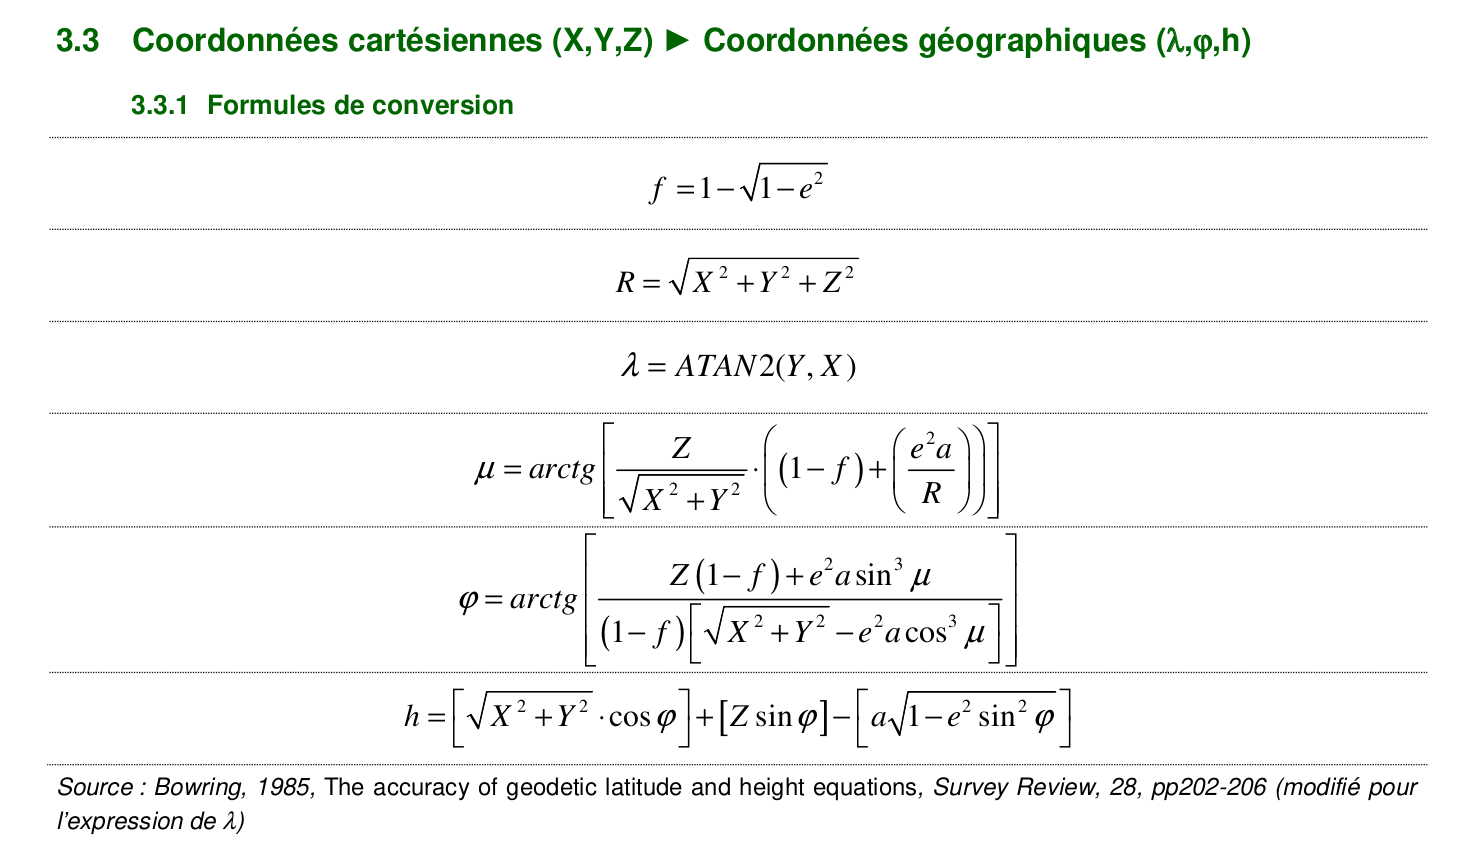
\includegraphics[width=16cm]{Programmer/GeoCtoGeoG.png}
\caption{Geocentric to geodetic coordinates}
\label{fig:GeoCtoGeoG}
\end{figure}

Since there is no vertical deflexion nor geoid model for now, we suppose that $H = h$.

%---------------------------------------------
%---------------------------------------------
%---------------------------------------------

\section{Handling constrained optimization}

%---------------------------------------------

\subsection{Theoretical aspect}

%  -  -  -  -  -  -  -  -  - -  -  -  -  -  -  -  -  - -  -  -  -  -  -  -  -  - -  -  -  -  -  -  -  -  -

\subsubsection{Introduction}

We consider the problem of minimizing $F(X)$ as in equation~\ref{EqNLOInit} under
the $n$ constraints:

\begin{equation}
	C_1(X) =0, \; C_2(X)=0 \dots \;  C_n(X)=0
\end{equation}

In  equation~\ref{EqNLOInit} we consider that the current solution is
close to the optimal solution and the equation can be linearized.
Similarly we consider that the current solution is close to the 
optimum under constraint, and consequently that the constraints are almost satisfied.
We consider then that the constraints can be linearized :

\begin{equation} 
C_k(X) \approx L_1 \cdot X  - c_k
\end{equation} 

So we can write :

\begin{equation} 
\begin{split}
  L_1 \cdot X = c_1 \\
  L_2 \cdot X = c_2 \\
    \dots \\
  L_n \cdot X = c_n 
\end{split}
\end{equation}

%  -  -  -  -  -  -  -  -  - -  -  -  -  -  -  -  -  - -  -  -  -  -  -  -  -  - -  -  -  -  -  -  -  -  -

\subsubsection{"Hard" vs "Soft" constraint}

What we call "soft" constraint is the method consiting in adding
the constraint as a penalization, with a certain weigthing $w$  in optimization:

\begin{equation}
    F_w(X) = F(X) + w  \sum_k (L_k-c_k)^2 \label{SoftConstraint}
\end{equation}

Soft constraints are just observations like others and do not require
to add any supplementary method. If what we want is hard constraints, an
easy way could be to use equation~\ref{SoftConstraint} with a "very high"
value for $w$.   Mathematically speaking, except for pathological cases,
generally when $w \rightarrow \infty$, the solution of ~\ref{SoftConstraint}
will converge to the solution of the hard constraint.

Although it can work, this cannot be a general method, because generally
it is difficult, if not impossible to define a \emph{"good very high $w$"}.
If it is not high enough, the solution will not be close enough to the hard
constraint.  It it is too high, it can create numerical inacuracy.

%  -  -  -  -  -  -  -  -  - -  -  -  -  -  -  -  -  - -  -  -  -  -  -  -  -  - -  -  -  -  -  -  -  -  -

\subsubsection{Lagrangian method}

To detail later : mention that it can be equivalent to solve the system with :

\begin{equation}
  \begin{pmatrix}
   A & L \\
   ^t L & 0 
  \end{pmatrix}
\end{equation}

But the system being no longer definite-positive, the resolution can be tricky.

%  -  -  -  -  -  -  -  -  -  -  -  -  -  -  -  -  -  - -  -  -  -  -  -  -  -  - -  -  -  -  -  -  -  -  -

\subsubsection{Substitution methods, case of $1$ constraint}
\label{CSTR:SUBST}

MMVII uses a substitution method. First, let's examine the case with $1$ variable, suppose:

\begin{itemize}
    \item we have a constraint $L \cdot X = c$;
    \item noting $L= (l_0,l_1 \dots)$ and suposing $l_0 \neq 0$,  note $L'=(l_1,l_2, \dots)$ and $X'=(x_1,x_2\dots)$;
\end{itemize}


The constraint can be written :
\begin{equation}
    x_0 = \frac{c-L' \cdot X'}{l_0} \label{LSQ:SUBST}
\end{equation}

Now  each time we add a new observation we will substitute $x_0$ :

\begin{itemize}
      \item let's note the observation  $Obs(X) = A \cdot X - C$
      \item with $A= (a_0,a_1 \dots)$, note  $A' = (a_1,a_2 \dots) $
       \item then   $Obs(x) = a_0 x_0 + A' X'-C= a_0\frac{c-L' \cdot X'}{l_0} + A'X' -C$
\end{itemize}

And finally:

\begin{equation}
    Obs(x) = (A'- \frac{a_0}{l_0} L') X'  - (C -c\frac{a_0}{l_0})
\end{equation}

So by doing the substitution for each observation we obtain a system with $N-1$ variables,
where $x_0$ has been eliminated, and without constraint. We can solve it, to find $x_1, x_2 \dots $,
and at the end, use equation~\ref{LSQ:SUBST} to find $x_0$.


%  -  -  -  -  -  -  -  -  - -  -  -  -  -  -  -  -  - -  -  -  -  -  -  -  -  - -  -  -  -  -  -  -  -  -

\subsubsection{Substitution methods, case of N constraints}
\label{CSTR:NSUBST}

We study the case with $2-3$ constraints, the generalization to $N$ constraints being straightforward.
Suppose we have two constraints $C_a$ and $C_b$ :

\begin{itemize}
    \item $C_a : L^a_0 x_0 +  L^a_1 x_1 \dots    = c^a$;
    \item $C_b : L^b_0 x_0 +  L^b_1 x_1 \dots    = c^b$;
\end{itemize}

For each observation, once we have made a substition with $C_a$ to eliminate $x_0$,
 we  want to use $C_b$ to eliminate $x_1$.
But for this we need to have $ L^b_0=0$, else it will "re inject" $x_0$.  To
force $L^b_0=0$, we remark  that for any $\lambda$ :

\begin{equation}
    C_a(X)=0  , C_b(X)=0   \Leftrightarrow  C_a(X)=0  , C_b(X)+\lambda C_a(X) =0
\end{equation}

So if we set $C'_b = C_b - \frac{L^b_0}{L^a_0} C_b$, we can now : use $C_a$ to eliminate $x_0$,
then use $C'_b$ to eliminate $x_1$. 

The idea is to make a "pre-processing" of constraints to allow a substitution in cascade.
If we have $3$ constraints $C_a, C_b, C_c$, we subract $C_a$ in $C_b$ and $C_c$, to have $C_a, C'_b, C'_c$
where $x_0$ is absent of $C'_b$ and $C'_c$. Then we substract  $C'_b$ to $C'_c$ to have a new constraint 
$C''_c$ where  $x_0$ and $x_1$ are eliminated.  For each observation, by substituting consecutively $C_a,C'_b,C''_c$, we can eliminate
$x_0$, $x_1$ and $x_2$.

This pre-processing of constraints is exactly the same than a gaussian elimination in linear resolution.
It requires some precaution to be stable, practically we make some "pivoting" to select the biggest coefficient
to eliminate.

%---------------------------------------------

\subsection{Using it in MMVII}

\label{Cstr:Use:MMVII}

%  -  -  -  -  -  -  -  -  -  -  -  -  -  -  -  -  -  - -  -  -  -  -  -  -  -  - -  -  -  -  -  -  -  -  -

\subsubsection{Restrictions/Potential Errors}

Although we think that this approach brings benefits, its use requires some precaution.
If not respected, it can rise several errors at execution of the program.

First and most important, the method requires that we know all the constraints
before any observation can be added.  This is handled by {\tt MMVII} using a boolean flag {\tt mInPhaseAddEq}.
This flag is set to {\tt false}  at the end of each iteration, and set to {\tt true} when
the first observation is added.  Once this flag is set to {\tt true}, no adding of constraint
will be allowed (see the method {\tt AssertNotInEquation}).

Another kind of error that can occur is to add too much constraints so that it becomes
impossible to comply with all of them. Of course this is not due to the way it is handled,
but is intrinsic to the notion of hard constraints. If this happens, an error
will be raised:

\begin{itemize}
     \item  see the method {\tt LinearMax} in class  {\tt cOneLinearConstraint};
     \item  an error with  message like {\tt "LinearMax probably bad formed constrained"} will be raised.
\end{itemize}

Note that this redundancy is detected from the structural point, not from the numerical point. For example
if we add $3$ constraints involving only the $2$ same unknowns an error will be detected; even if it is
$3$ times the same constraint (numerically it can be satisfied because if it's $3$ time the same, it is in
fact a constraint $1$ constraint, but "structurally" \emph{too many constraint for unknowns} will be detected).


Conversely, for example if $x$ and $y$ are unknown, if we add the $2$ constraint $x+5y=1$ and $\frac{x}{3}+ \frac{5y}{3}=0$,
in exact arthimetic it's is impossible to comply with these two constraint; but due to rounding error, it's likely
that no contradiction will be detected by the programm (but we will have a very unstable elimination).

%  -  -  -  -  -  -  -  -  -  -  -  -  -  -  -  -  -  - -  -  -  -  -  -  -  -  - -  -  -  -  -  -  -  -  -

\subsubsection{Handling "frozen" variables}

The most current use of constraint is the case where we want to impose that a given unknown
has a given value (its current value or a new value). The constraint is simply
$X_i=C$.   There are several methods to facilitate this manipulation in class {\tt cResolSysNonLinear}, for
the freezing part we have:

\begin{itemize}
     \item   {\tt SetFrozenVarCurVal(int aK)} freezes the value of an unknown to its current value,
              knowing the number of the unknown in the system;
     \item   {\tt SetFrozenVarCurVal(tObjWUk \& anObj,const  Type \& aVal)}, idem, but specify the object {\tt anObj}
	     and the adress of the value {\tt aVal} that must be \emph{"inside"} the object;
     \item  several variants freezing several unkowns of an object (using points or adresses + a number) or all the
            object;
      \item  {\tt SetFrozenVar(int aK,const  Type \&)}, to force an unknown to have a given value
             (i.e. \emph{a priori} different from its current value).

\end{itemize}

For the unfreezing part we have some similar methods:

\begin{itemize}
	\item   {\tt SetUnFrozen(\dots)} suppresses the constraint of an unknown (idem, with method knowing its number
		and method with an object and one address);
      \item  {\tt UnfrozeAll()} suppresses all the constraints on freezing any variable.
\end{itemize}

%  -  -  -  -  -  -  -  -  -  -  -  -  -  -  -  -  -  - -  -  -  -  -  -  -  -  - -  -  -  -  -  -  -  -  -

\subsubsection{Handling "shared" unknown}

Sometimes it occurs  that for a set of unknwons, theoretically different,  we want to enforce
temporarilly these unknowns to have the same value: that's what we call shared unknowns. 
A possible example is with several cameras where we want each camera to have its own focal length
but want them to have the same distorsion, and this distorsion
has to be adjusted.  \emph{unknown sharing} will allow to do that without requiring to add a specific model of camera.

From the theoretical point of view, it's quite direct to impose shared unknowns  with constrained optimization.  For forcing
$n$ unknows to have a shared value : $X0=X1=X2\dots=X_{n-1}$, we simply add $n-1$ equations selecting
an arbitrary reference variable $X_0$ : $X_0-X_1=0$, $X_0-X_2$=0, \dots , $X_0-X_{n-1}=0$.
The methods in class {\tt cResolSysNonLinear} for manipulating shared unknown are:

\begin{itemize}
    \item   {\tt SetShared(const std::vector<int> \&  aVUk)}  given a vector of unknowns numbers,
            make them a set of unkowns shared;
    \item   {\tt SetUnShared(const std::vector<int> \&  aVUk)} make the invert operation;
    \item   {\tt SetAllUnShared()} 
\end{itemize}

An example of a combination of {\tt Frozen} and {\tt Shared} unknowns can be found in {\tt LinearConstr} bench function {\tt BenchFrozenAndShare()}.

%  -  -  -  -  -  -  -  -  -  -  -  -  -  -  -  -  -  - -  -  -  -  -  -  -  -  - -  -  -  -  -  -  -  -  -

\subsubsection{Handling general case, linear and non linear}

Beside the special case of unknowns freezing or sharing, there are methods for handling general constraints.
For the linear case we have the method {\tt AddConstr} :

\begin{itemize}
    \item {\tt AddConstr(const tSVect \& V,const Type \& C,bool OnlyIfFirstIter=true);}
    \item  {\tt V} is the linear part , {\tt C} is the constant, it correspond to the equation $ V \cdot X = C$ ;
    \item  the parameter {\tt  OnlyIfFirstIter} indicate that the constraint must be added only if we are at the
           first iteration of the non linear system.
\end{itemize}

For non linear constraints we have the method {\tt AddNonLinearConstr}.  It's very similar to {\tt CalcAndAddObs}
(see \ref{AddBasicEq}), it takes a calculator corresponding to a funcion $F$ to compute the value 
and its derivatives and generate a linearized version of the constraint $F(X)=0$:

\begin{itemize}
    \item {\tt  void AddNonLinearConstr(tCalc * aCalcVal,const tVectInd \& aVInd,const tStdVect\& aVObs,bool  OnlyIfFirst=true);}

    \item  {\tt aCalcVal,aVInd, aVObs} play the same role than  in {\tt CalcAndAddObs};

    \item  the parameter {\tt  OnlyIfFirstIter} play the same role than in {\tt AddConstr}. 
\end{itemize}

The method {\tt SupressAllConstr()} suppresses all the constraints
added by {\tt AddConstr}  or {\tt AddNonLinearConstr}.

%  -  -  -  -  -  -  -  -  -  -  -  -  -  -  -  -  -  - -  -  -  -  -  -  -  -  - -  -  -  -  -  -  -  -  -

\subsubsection{Example in bench}

In the network bench the method {\tt AddGaugeConstraint} gives examples of using 
the constraints to fix the arbitrary rotation that cannot be fixed by distance conservation.
It also serves as an unit test of correctness.  The "natural" way, already described, is to fix
$3$ coordinates $X_{0,0},Y_{0,0},X_{1,0}$ with soft or hard constraints (using  {\tt AddEqFixVar} or  {\tt SetFrozenVar}).

The other tested methods are completely artificial and activated with the flag {\tt doMangleCstr},
this test is done using constraints involving the neighborhood of a point.
Let $X_k$ be the unknowns of the neighbouring points, and $R_k$  be the 
ground truth value of the $X_k$.

For testing the linear constraints, with {\tt AddConstr} we generate a random weighting $W_k$
and we add the linear constraint:

\begin{equation}
    \sum_k W_k  X_k = \sum_k  W_k  R_k  
\end{equation}

For the non linear constraint, we use the following equation:

\begin{equation}
    \sum_k  X_k^2 = \sum_k   R_k^2
\end{equation}

%---------------------------------------------

\subsection{Implementation details}

%  -  -  -  -  -  -  -  -  -  -  -  -  -  -  -  -  -  - -  -  -  -  -  -  -  -  - -  -  -  -  -  -  -  -  -

\subsubsection{Global presentation }

This part is for the programmer that will need to maintain and make evolve the core system.
For the programmer that "only" want to use it in optimisation in {\tt MMVII}
the interaction with {\tt cResolSysNonLinear}, described 
in \ref{Cstr:Use:MMVII}, is sufficient.

The code relative to constrained optimization is located in the files {\tt Matrix/LinearConstraint.h}
and  {\tt Matrix/cLinearConstraint.cpp}. The classes involved are:

\begin{itemize}
    \item  {\tt cOneLinearConstraint}  for representing a single constraint;
    \item  {\tt cSetLinearConstraint}  for representing a set of constraint  : initial value and value after
           pre-processing described in~\ref{CSTR:NSUBST};
    \item  {\tt cDSVec}   helper class allowing easy manipulation of sparse vector;
    \item  {\tt cBenchLinearConstr}   class for doing some unitary test on {\tt cSetLinearConstraint}.
\end{itemize}

%  -  -  -  -  -  -  -  -  -  -  -  -  -  -  -  -  -  - -  -  -  -  -  -  -  -  - -  -  -  -  -  -  -  -  -

\subsubsection{Class {\tt cDSVec} }

By itself the method of subsitution is relatively simple. But there is some complexity added 
for efficient implementation :

\begin{itemize}
    \item  in many context where non linear optimization is used, including photogrammetry,  each observation
           imply few unknowns (says $\approx 10-50$)  among many (say $\approx 500-100000$);

    \item  for efficient representation we use sparse vector for constraint and observation, 
           a sparse vector being a collection of pair index/value;

     \item let name $m$  the number of pair of a sparse vector and $N$ the number of unknowns;

    \item  many operation on sparse vector, like substitution described in~\ref{CSTR:NSUBST}, require some
           precaution if we want that the cost to be in $\mathcal{O}(m)$  rather than in $\mathcal{O}(N)$.
\end{itemize}


This is here that  {\tt cDSVec}  can help. It is a class for dense representaion of sparse vector. Typically a  {\tt cDSVec}:

\begin{itemize}
    \item  contains a dense real vector $V$ (initialy full of $0$), a list of used indexes $L$ (initially empty), a dense boolean
           vector indicating if the index is used $B$ (initially full of false) 
    \item  each time an element is added-suppressed on the {\tt cDSVec} at index $i$, the dense vector is updated 
           at $V[i]$ and if $B[i]$ is false (meaning it has not been used) then $B$ and $L$ are also updated;
    \item  a {\tt cDSVec} can be quickly reset to its initialvalue, by parsing $L$ to : set $V$ to $0.0$, set $B$ to false,
            and finally clearing $L$.
    
\end{itemize}

Typically, as the allocation of a dense vector can take some time (in  $\mathcal{O}(N)$) the idea is to allocate
a dense vector in class {\tt cSetLinearConstraint} and to reuse it many times and reset it at the end of each use
(that's a buffer).


%  -  -  -  -  -  -  -  -  -  -  -  -  -  -  -  -  -  - -  -  -  -  -  -  -  -  - -  -  -  -  -  -  -  -  -

\subsubsection{Class {\tt cOneLinearConstraint} }


The class {\tt cOneLinearConstraint} is used to represent one linear constraint (who would believe that !! \dots  :-;).
It contains a sparse vector {\tt mLP}$=V$ and a constant {\tt mCste}$=C$. At its creation it
represents directly the constraint  $V \cdot X = C$.

Once it has been "reduced" (i.e. the substitution described in  \ref{CSTR:SUBST} has been applied),
the {\tt mISubst}$=i$ contains the number of the unknowns to substitute, and {\tt mLP}$=V'$ no longer the
pair containing $I$, the constraint is then $V' \cdot X + X_i = C$.  The boolean {\tt mReduced}
indicate if the constraint was reduced.

%  -  -  -  -  -  -  -  -  -  -  -  -  -  -  -  -  -  - -  -  -  -  -  -  -  -  - -  -  -  -  -  -  -  -  -

\subsubsection{Class {\tt cSetLinearConstraint} }

The class {\tt cSetLinearConstraint} is the  main class, i.e the only class the
"rest of the word" needs to interact with. It contains essentially the following data:

\begin{itemize}
    \item  a copy of the initial version of the constraints;
    \item  a copy of reduced versions;
    \item  a bufffer of type {\tt cDSVec} to accelerate the computation;
\end{itemize}

A typical sequence of use will be:


\begin{itemize}
    \item   create the object, indicating the number of unknowns (to allocate the buffer);
    \item   add a number of $M$ constraints (using {\tt Add1Constr} or {\tt Add1ConstrFrozenVar});
    \item   "compile" the object, this means apply the processing of~\ref{CSTR:NSUBST} to create the
	    reduced constraint in {\tt mVCstrReduced};
    \item   each time an observation is added, use one of the $3$ following methods to eliminate the $M$ variables 
	    selected in {\tt Compile} :
	    \begin{itemize}
                 \item {\tt SubstituteInSparseLinearEquation}; 
                 \item {\tt SubstituteInDenseLinearEquation} 
                 \item {\tt SubstituteInOutRSNL}
	    \end{itemize}
    \item    use the method {\tt void AddConstraint2Sys(tLinearSysSR \&)}, this method simply add all the constraint
             as linear observation, this is necessary to fix the value of the substituted unknowns (because by 
             construction they have been eliminated).

\end{itemize}







\include{Programmer/SymbolicDerivation}


\include{Programmer/Mapping}



%   ------------------------------------------------------------------
%   ------------------------------------------------------------------
%                 Chapter Interpolators
%   ------------------------------------------------------------------
%   ------------------------------------------------------------------

\chapter{Interpolators in \PPP}

\label{ChapInterpolators}

    % = = = = = = = = = = = = = = = = = = = = = = =
    % = = = = = = = = = = = = = = = = = = = = = = =
    % = = = = = = = = = = = = = = = = = = = = = = =

\section{Introduction}
This chapter groups the functionnality added in \PPP for image interpolation. In this
first draft different view-points are merged in the same chapter : theory, users, programmers,
and finally mainteners of the core-\PPP.  This organization may evolve with dispatching of different section
of this chapter in different part.

The following header  files , in {\tt include/} are involved in interpolators declaration :

\begin{itemize}
    \item {\tt MMVII\_Interpolators.h } : main file, contains the declaration of interpolators class;
    \item {\tt MMVII\_Images.h} ,{\tt MMVII\_Image2D.h} declaration of methods involving interpolators
          in images;

    \item {\tt MMVII\_TplSymbImage.h}  declaration of method using interpolators in image differentiation
          (as alternative to bilinear mode).
\end{itemize}

The following source  files , in {\tt src/} are involved in interpolators definition :

\begin{itemize}
   \item {\tt UtiMaths/Interpolators.cpp} definition of interpolator classes;
   \item {\tt ImagesBase/cIm2d\_Interpolators.cpp} definition of methods for interpolating $2-d$ images with
         \PPP's interpolators;
   \item {\tt Bench/BenchInterpolators.cpp}  definition of method for checking correctness of implementation
         (unitary test);

   \item {\tt Bench/BenchTutoImageDef.cpp} contains the test for image differenciation, initially made for bilinear mode,
         has been extended to take into account  interpolators.
\end{itemize}


    % = = = = = = = = = = = = = = = = = = = = = = =
    % = = = = = = = = = = = = = = = = = = = = = = =
    % = = = = = = = = = = = = = = = = = = = = = = =

\section{Theoreticall background}

\subsection{introducion}

Theory of image/signal interpolation is an essential  part of image processing and there is a huge 
documentation on the subject. The very brief theoreticall elements given here are more targeted to fix notation
than to be a complete summary of the theory.

In the more general case, in interpolation we have a function $F$  of $\RR^n$ sampled on a finite  set $p_k,v_k$
\footnote{or countable and isolated} set of point and we want to extend the value to whole
$\RR^n$  using some  property on $F$ :

\begin{itemize}
   \item $F$ is regular enough, whatever it means;
   \item $F(p_k) = v_k$ if we require a perfect match, or $F(p_k) \approx v_k$  if require only a close
         match,  whatever it means;
\end{itemize}



In the case of image/signal processing, we suppose that we know the value on regular grid $\{p_k\}=\ZZ^n$
and want to extand $F$ from $\ZZ^n$ to whole $\RR^n$ . 
Considering for know, a $1d$ interpolation, we have $p_k=k$, we note $\Interpol :  {v_k}  \rightarrow F$ 
the interpolation process.  

    % = = = = = = = = = = = = = = = = = = = = = = =

\subsection{$1d$ interpolation kernel}

We generally assume the following properties ,linearity as in~\ref{IntLin} :

\begin{equation}
    \Interpol_{\{a*v_k+b*w_k\}} = a*\Interpol_{\{v_k}\}+ b*\Interpol_{\{w_k\}} \label{IntLin}
\end{equation}

Invariance by translation, which mean that is we translate globally the $v_k$ of an integer $n$
we must translate the function of $n$ :

\begin{equation}
    \Interpol_{\{v_{k+n}\}}(x) =  \Interpol_{\{v_{k}\}}(x+n)  \label{IntTrans}
\end{equation}

The property of equation \ref{IntLin} and \ref{IntTrans}, have for consequence that interpolation
can be entirely caracterized by "kernel" function $\KernI : \RR \rightarrow \RR $ such that :

\begin{equation}
    F(x) =  \Interpol_{\{v_{k}\}}(x) = \sum_{k}  v_k  \KernI(x-k)   \label{KernIntDef}
\end{equation}

To assure the  integrity of interpolation process we generally assume properties on $\KernI$
such as $\KernI$ is continous (or differrentiable) and  $\int_{\RR} \KernI ^2 $ is defined. We dont
discuss in detail these "natural" hypothesis.
We generally assume a symtetry hypethosis on interpolation that can be traduced in symetry on
$\KernI$ :

\begin{equation}
    \KernI(-x) =   \KernI(x)   \label{KernIntSym}
\end{equation}


A "natural" property of interpolation is that if the value $v_k$ are constant $v_k=c$, the interpolated function 
is constant $F(x)=c$ . From the kernel point of view this property is traduced as the \emph{aka} partition of unity :

\begin{equation}
    \forall x \in \RR : \sum_k \KernI(x+k) =   1 \label{PartUnit}
\end{equation}


The constraint that the intepolation coincide with values on sample point ($F(k)=v_k$) if it
applies  is traduced by equation (where $\delta_x$ is kronecker's symbol) meaning that $ \KernI$ must
be null for any non null integer value, and must value $1$ for $k=0$ :

\begin{equation}
    \forall k \in \ZZ :  \KernI(k) =   \delta_0 \label{KernIntDelta0}
\end{equation}

For practicall reason, we cannot compute infinite sum like in equation~\ref{KernIntDef}, and we 
generally make the hypothesis that the support of $\KernI$ is bounded by a certain value $Sz_K$ :


\begin{equation}
    \forall x \in \RR   :  |x| > Sz_K  \Rightarrow \KernI(x) = 0 \label{KernIntBounded}
\end{equation}

    % = = = = = = = = = = = = = = = = = = = = = = =

\subsection{N-dimentional interpolation}

    %    -  -  -  -  -  -  -  -  -  -  -  -  -  -  -  -  -  -  -  -  -  -  -  -  -  -  -  -  -  -  -  -  -  -  -  -
\subsubsection{Separable kernels}

To keep things simple, we describe the interpolation on a $2$ dimensionnal grid $\ZZ^2$ wich is
usefull for image processing, but generalization to  higher dimension is obvious. For $N-d$
interpolation, we the same hypothesis than for $1d$ on linearity and invariance by translation we
can deduce the existance of a kernel function $\KernI(x,y)$ such that :

\begin{equation}
    F(x,y) =  \Interpol_{\{v_{i,j}\}}(x,y) = \sum_{i,k}  v_{i,j}  \KernI(x-i,y-j)   \label{KernInt2DDef}
\end{equation}

We generally make the separability hypothesis, this hypothesis says in general that interpolation
in $x,y$ can be done from the interpolation in $x$ of the sample interpolated in $y$. For a interpolation 
kernel , this is traduced as :

\begin{equation}
     \KernI(a,b)  = \KernI_x(a) \KernI_y(b)  \label{KernIntSep} 
\end{equation}

Where $\KernI_x$ and $\KernI_y$ are the interpolation kernels for $x$ and $y$. Also in general $x$ and $y$ play
the same role, which the case in image processing and we have :

\begin{equation}
      \KernI_x(a) =  \KernI_y(a)  \label{KernIntSymSep} 
\end{equation}

So finally we have the equation :

\begin{equation}
    F(x,y) =   \sum_{i,j}  v_{i,j}  \KernI(x-i) \KernI(y-j)   \label{KernInt2DDef}
\end{equation}

    %    -  -  -  -  -  -  -  -  -  -  -  -  -  -  -  -  -  -  -  -  -  -  -  -  -  -  -  -  -  -  -  -  -  -  -  -
\subsubsection{Synthesis}

We can make a brief synthesis of interpolation model we use in \PPP,  the interplation of an image $v_{i,j}$ can
be computed by following formula :

\begin{equation}
    F(x,y) =  \sum_{i,j}  v_{i,j}  \KernI(x-i) \KernI(y-j)   \label{IntIm2D}
\end{equation}


Where the kernel  $\KernI$ is a  $\RR \rightarrow \RR$ function with the following properties :

\begin{itemize}
    \item  $\KernI$ is regular (continous at least) and $\int_{\RR} \KernI^2$ is finite;
    \item  $\KernI$ is symetric (see \ref{KernIntSym});
    \item  $\KernI$ complies with partition of unity property (see \ref{PartUnit});
    \item  $\KernI$ is \emph{generally} such that $F(x,y)$ coincide with $v_{x,y}$ for integer
           values of $x,y$, which lead to  equation \ref{KernIntDelta0} ;
    \item  $\KernI$ is \emph{practically} bounded to an interval $Sz_K$ as in equation~\ref{KernIntBounded}.
\end{itemize}

    %    -  -  -  -  -  -  -  -  -  -  -  -  -  -  -  -  -  -  -  -  -  -  -  -  -  -  -  -  -  -  -  -  -  -  -  -
\subsubsection{Remark on implemantaion efficiency}

\label{InterpValueEff}

Obviously, in equation~\ref{IntIm2D} we can  restrict the sum to $i \in [x-Sz_K,x+Sz_k]$, and
idem for $j$. This said, a "naive" implementation of~\ref{IntIm2D}, can lead
to $2*(1+2*Sz_K)^2$ evaluation of $\KernI$. 

A basic optimization consist to use the separability and write :

\begin{equation}
    F(x,y) =  \sum_{j}  \KernI(y-j)   \sum_{i}  v_{i,j}  \KernI(x-i)  \label{IntIm2DOpt}
\end{equation}

Now if, before entering the main loop, we pre-compute in a table the value of $\KernI(x-i)$,  
we will just need to  compute once the $\KernI(y-j)$ and $\KernI(x-i)$

    % = = = = = = = = = = = = = = = = = = = = = = =

\subsection{Derivate the interpolation}

\label{InterpDeriv}

When the image is considered as function of $x,y \in \RR^2$, interpolation by kernel
offer not only the possibity to get the value for real coordinates, but also a \emph{natural}
and relatively efficient, way to compute the exact derivatives, provide that $\KernI$ is
a differentiable funcion. Noting :

\begin{equation}
       \KernI' =  \frac{\partial \KernI(x)}{\partial x}  \label{DefDerKern}
\end{equation}

Going back to equation \label{KernIntDef}, we have :


\begin{equation}
    F'(x)  = \sum_{k}  v_k  \KernI'(x-k)   \label{KernIntDeriv1D}
\end{equation}

Equation show that we can compute the derivative of interpolated function
with a formula similar to  interpolation where $\KernI'$ replace $\KernI$.
Let study then briefly the properties of $\KernI'$ when 
 $\KernI$ is a differentiable interpolation kernel :

\begin{itemize}
   \item  $\KernI'$ is bounded on the same support than $\KernI$;
   \item  $\KernI'$ is an odd function because $\KernI$ is an even function;
   \item  if $\KernI$ is a partition of unity (equation~\ref{PartUnit}) then $\KernI'$ complies with equation  ~\ref{PartZero};
\end{itemize}

\begin{equation}
    \forall x \in \RR : \sum_k \KernI'(x+k) =   0 \label{PartZero}
\end{equation}

For $2d$ interpolation, we have similarly :

\begin{equation}
    \frac{\partial F(x,y)}{\partial x} =  \sum_{i,j}  v_{i,j}  \KernI'(x-i) \KernI(y-j)   \label{Int2DerX}
\end{equation}

And  :
\begin{equation}
    \frac{\partial F(x,y)}{\partial y} =  \sum_{i,j}  v_{i,j}  \KernI(x-i) \KernI'(y-j)   \label{Int2DerY}
\end{equation}

Note also, that very often when need derivates, we need simultaneaously the $3$ values $F(x,y), \frac{\partial F(x,y)}{\partial x}$
and  $\frac{\partial F(x,y)}{\partial y}$, it is advantageaous then to compute the $3$ value in the same function, because
a shown by equations~\ref{InterpSimultComp} several computation can be shared :

\begin{itemize} 
    \item obviously share the loops on $i,j$;
    \item share the tabulation of $\KernI(y-j)$;
    \item share the computation of $\sum_{i}  v_{i,j}  \KernI(x-i)$.
\end{itemize} 

\begin{equation}
\left\{ \begin{array}{rcl}
     F(x,y)                                    &   \mbox{=} &  \sum_{j} \KernI(y-j)  \sum_{i}  v_{i,j}  \KernI(x-i)   \\
      \frac{\partial F(x,y)}{\partial x}       &   \mbox{=} &  \sum_{j} \KernI(y-j)  \sum_{i}  v_{i,j}  \KernI'(x-i)  \\
      \frac{\partial F(x,y)}{\partial y}       &   \mbox{=} &  \sum_{j} \KernI'(y-j) \sum_{i}  v_{i,j}  \KernI(x-i)  
\end{array}\right.
\label{InterpSimultComp}
\end{equation}

    % = = = = = = = = = = = = = = = = = = = = = = =
\subsection{Standard interpolation kernel used in \PPP}

All the standard intepolator complies with equation~\ref{KernIntDelta0}.

   %   -  -  -  -  -  -  -  -  -  -  -  -  -  -  -  -  -  -  -  -  -  -  -  -  -  -  -  -  -  -  -  -  -  -  -  -
\subsubsection{Nearest neighboor interpolation kernel}

\emph{Not implemented for now} because it has very poor property (not even continous), but may be added 
(for test/comparison ?).

The kernel has support $S=]-\frac{1}{2},\frac{1}{2}]$ and we have $\KernI(x)=1$/

   %   -  -  -  -  -  -  -  -  -  -  -  -  -  -  -  -  -  -  -  -  -  -  -  -  -  -  -  -  -  -  -  -  -  -  -  -
\subsubsection{Linear interpolation kernel}
\label{LinearInterp}

The linear interpolator has support $[-1,1]$ and is defined by the following kernel :

\begin{equation}
  \KernI(x)= |1-x|
\end{equation}

It is continous but not derivable.


   %   -  -  -  -  -  -  -  -  -  -  -  -  -  -  -  -  -  -  -  -  -  -  -  -  -  -  -  -  -  -  -  -  -  -  -  -
\subsubsection{Sinus Cardinal interpolation kernel}
\label{SinCInterp}


In it's  "pure" definition it's an unbounded interpolator defined by :

\begin{equation}
  \KernI(x)= \sinc(\pi x) = \frac{\sin(\pi x)}{\pi x}
\end{equation}

It's $C_{\infty}$ and is interesting from the theoreticall point of view as it allows
to recover exactly the  function from its sampling if the function complies with \emph{Nyquist-Shannon}
hypothesis. Practically no realistic function complies with \emph{Nyquist-Shannon},   but
it still remain interesting as a model when we require the "best ressampling possible".

The function $\sinc$  veririfies equation  \ref{PartUnit} (reference for this non obvious property ??).


   %   -  -  -  -  -  -  -  -  -  -  -  -  -  -  -  -  -  -  -  -  -  -  -  -  -  -  -  -  -  -  -  -  -  -  -  -
\subsubsection{Apodized Sinus Cardinal interpolation kernel}
\label{SinCApodInterp}


A practicle limitation of $\sinc$-kernel is its infinite support that makes it impossible to use as is.  
By the way, it remains an interesting option for these reconstruction aspect.  Also, "cuting" brutally
the $\sinc$ to have a bounded kernel is not a good idea as it would creat high frequency, so generally
we use an "apodization" function $A$ that generate a smooth transition, typically we will have :

\begin{itemize}
    \item $A(x)=1$  for $x \in [0,a] $
    \item $A(x)$  decrease continuoussly from $1$ to $0$ for  $x \in [a,a+b] $, a basic example is
          $A(x) = L_{a,b}(x) = \frac{b-x}{b-a}$, but can take also a smoother version as $Cub_0 \circ L_{a,b}$
          where $Cub_0$ is the cubic function of parameter $0$ (see \ref{CubicInterpol});
\end{itemize}

The  $\sinc$ apodized is then defined by :

\begin{equation}
  \KernI(x)  = A(x) \sinc(\pi x)  \label{SinCApod}
\end{equation}

The formula cannot be used as is, because if $\sinc$ complies with~\ref{PartUnit}, it's no
more the case of $\sinc * A$, an eathy way to overcome this issue (and work for any kernel) is
to replace by the normalized kernal $\KernI^n$:

\begin{equation}
  \KernI^n(x)  =  \frac{\KernI(x)}{\sum_{k \in \ZZ} \KernI(x+k)} \label{InterNormKern}
\end{equation}

However we have then $2$ other issue :

\begin{itemize}
   \item  computation of formula~\ref{InterNormKern} can be a time-consuming ;
   \item  derivation of formula~\ref{InterNormKern}, as required in~\ref{InterpDeriv} 
          for dervivation of intepolated function, can become quite complex.
\end{itemize}

Concretely, these issues can be addressed efficiently  using a \emph{tabulated} implementation
of the apodized $\sinc$ as described in~\ref{InterpolTabul}.


   %   -  -  -  -  -  -  -  -  -  -  -  -  -  -  -  -  -  -  -  -  -  -  -  -  -  -  -  -  -  -  -  -  -  -  -  -

\subsubsection{Cubic interpolation kernel}

\label{CubicInterpol}



Cubic intepolation is a current choice as a compromise "quality/efficiency" : it is derivable and has a kernel of $2$ .
Each cubic interpolator if define by a parameter $p$ which is the value of derivate in $1$, we have :

\begin{equation}
\KernI(x) = Cub_p(x)
\left\{ \begin{array}{rcl}
(p+2 ) x^3 -(p+3)x^2+1        &   \mbox{for} &  0 \leq x \leq 1 \\ 
p*(x^3 - 5 * x^2 + 8* x -4)   &   \mbox{for} &  1 \leq x \leq 2 \\
0                             &   \mbox{for} &  2 \leq x \\
\KernI(-x)                    &   \mbox{for} &   x \leq 0 \\
\end{array}\right.
\end{equation}


The cubic interpolator has following properties :

\begin{itemize}
    \item  it is derivable, it suffice to check that $\frac{\partial Cub_p(x^-)}{\partial x} = \frac{\partial Cub_p(x ^+)}{\partial x} $  
           for $x \in \{0,1,2\}$;
    \item  it complies with proterties \ref{KernIntBounded},   \ref{PartUnit} and \ref{KernIntDelta0}  
\end{itemize}


For theoreticall reason (which ??) , the parameter $p$ should be in $[-3,0]$ . Some remarq on parameter $p$ :

\begin{itemize}
    \item  when used in image ressampling, the higher value of  $p$ enhance the high frequency of images, which can be used
           for zooming (upscaling) images ;

    \item  for  $p=0$  the support is $[0,1]$ and $\KernI(x) \geq 0$ , it can be used for image downscaling,
           it can be seen as an approximation of gaussian with small support;

    \item  for  $p= -0.5$  the interpolator  is such that interpolation of purely linear images (as $I(x,y)=a+bx+cy$)
           will  be linear; in some way, it will be the default choice when 
\end{itemize}

    % = = = = = = = = = = = = = = = = = = = = = = =
\subsection{Non Standard interpolation kernel used in \PPP}

\label{MMVIIInterpol}

The origin of these interpolator go back to the analysis of existing bias when using interpolation
in image correlation : in a context where the phase should theoretically be uniformly 
distributed in $[0,0.5]$ we  observe that some phase are "privilegied"  (?? which one, experience to be done ??).

The bias is particularly important with bilinear interpolator, a possible
analysis of these fact is the following :

\begin{itemize}
    \item  the "bluring" effect of the interpolator varies with the phase;
    \item  if the phase is $0$, the pixel will be a single pixel value 
    \item  if the phase is $\frac{1}{2}$, the pixel will be the average of two
           pixel, having a slight blurring effect.
\end{itemize}

To try to overcome this problem, we use the following reasonning :

\begin{itemize}
    \item  for phase  $\frac{1}{2}$, there is no much more to do than to have
           a weigting $0.5,0.5$ for the $2$ nearest neighboor if we want to limit the number of neigboors
           involved;
    \item  for phase  in $x \in [0,0.5]$ , we want to limit the size of kernel,
           but need to add at least a third pixel if we want to have weightin
           that is centered on $x$ and has the same bluring effect than for phase $\frac{1}{2}$;
    \item  regarding the blurring effect, it is caracterized as the average of the power $\alpha$ of 
           to the center distance , where $\alpha$ is parameter of the kernel (for $\alpha=2$ it's the
           variance);
     \item let's name $a,b,c$ the weighting of pixels $-1$, $0$ and $1$ for phase $x \in [0,0.5]$, the value
           of $a,b$ and $c$ can be evaluated by equations~\ref{KernInMMVIIEq}
\end{itemize}

\begin{equation}
\left\{ \begin{array}{rc|l}
  a+b+c        &    = 1  &  \textrm{it's a weigthing}  \\ 
  -a+c      &       = x &   \textrm{center is on } x \\
  a(1+x)^\alpha        + b x^\alpha +c(1-x)^\alpha & = \frac{1}{2} ^{\alpha} &  \textrm{maintain } \alpha  \textrm{-average of distance}
\end{array}\right.
\label{KernInMMVIIEq}
\end{equation}

For $\alpha=2$, the equations~\ref{KernInMMVIIEq} lead to a simple analyticall formula for the kernel :

    % if (anX<=0.5)  return 0.5 *(1.5-2*Square(anX));
    % if (anX<=1.5)  return 0.5 * Square(anX-1.5) ;

\begin{equation}
\KernI(x) = M_2(x)
\left\{ \begin{array}{rcl}
\frac{1.5-2x^2}{2}       &   \mbox{for} &  0 \leq |x| \leq \frac{1}{2} \\ 
\frac{(x-1.5)^2}{2}       &   \mbox{for} &  \leq \frac{1}{2} \leq |x| \leq \frac{3}{2} \\ 
0                             &   \mbox{for} &  |x| \geq \frac{3}{2}
\end{array}\right.
\label{KernInMMVII2Eq}
\end{equation}

For other value of $\alpha$ , the expression is not so simple, by the way if we need to use/test 
different value, we proceed this way :

\begin{itemize}
     \item we have a numerical version of the parametrized that for each phase solve the system 
           equations given in~\ref{KernInMMVIIEq};
     \item this numerical version  is relatively slow, but it's not a problem if we use the
           tabulated version as described in~\ref{InterpolTabul}.
\end{itemize}


    % = = = = = = = = = = = = = = = = = = = = = = =
\subsection{Tabulated interpolators}
\label{InterpolTabul}


As interpolation  kernel are $1$ dimensionnal bounded function, their value can be easily tabulated, this
means :

\begin{itemize}
    \item  fix a number $Nb$  of value per unity ;
    \item  create a tab $T$ of size $Nb*Sz_K$ ;
    \item for $K \in [0,Nb*Sz_K]$  set  $ T[K] = \KernI(\frac{K}{Nb})$
    \item when required to compute $\KernI(x)$  we simply extract the value of $T[x*Nb]$,
          preferably using bilinear interpolation.
\end{itemize}

Let note $T_\KernI$  the interpolator obtained by reading the values  $T[x*Nb]$.

First note that this technique can be accurate for relatively small cost in memory and accuracy:

\begin{itemize}
     \item typically consider the apodidzed sinus carninal with a kernel of $5$ and an apodiszation of $5$, tabulated with $Nb=1000$;
     \item the  cost in memory is $10000=(5+5)*1000$ elements, the cost of pre-computation is also $10000$  value;
     \item the  accuracy, i.e max difference between $\KernI$ and the tabulation value can be estimate to $\frac{1}{Nb^2} = 10^{-6}$
           (classical formula for accuracy of linear interpolation).
\end{itemize}

Having seen that the lost is low, see now what is the gain :

\begin{itemize}
    \item first obvious gain is time of computation of each new value ;

    \item second gain is that, once all the value has been stored in the tab, it's possible to do a post-processing
          using formula  similar to~\ref{InterNormKern} on the tabulated value; so finnaly $T_\KernI$ will 
          complies with unity partition formula (\ref{PartUnit});

    \item finnaly its possible to use $T$ for computing approximate values of derivates using formula
          like  $\frac{\partial T_\KernI}{\partial x} \approx \frac{T[k+1]-T[k-1]}{2*Nb}$, so we can
          make $T_\KernI$ differentiable, even if no analytical derivate is furnished for $\KernI$
          (but obvioulsy if $\KernI$ is intrinsically not differentiable, like linear interpolator, the
           results will be meanignless).
\end{itemize}

    % = = = = = = = = = = = = = = = = = = = = = = =
    % = = = = = = = = = = = = = = = = = = = = = = =
    % = = = = = = = = = = = = = = = = = = = = = = =

\section{Choice of an Interpolator}

    % = = = = = = = = = = = = = = = = = = = = = = =

\subsection{Interpolator for image up-izing}

Interpolator are mainly usefull for image resampling.  When the resampling is done
to a higher resolution, or a resolution equivalent the choice of an interpolator,
there is no so much to say, and it is mainly an affair of trade-off between accuracy and efficiency :

\begin{itemize}
   \item for fast computation and low accuracry, bi-linear can be a good choice;
         it's not recommanded when derivative are required;

   \item bi-cubic can be a good compromize quality/efficiency, the default recommander
         parameter being $P=-\frac{1}{2}$, but higher value can be used for image enhancing
         when used at high zooming;

   \item for "best" ressampling, with minimal aliazing, according to signal theory, the sinus cardinal
         can be used;

   \item finally, in image correlation the non standard interpolator \ref{MMVIIInterpol}, especially $M_2$,
         can be interesting compromize.

\end{itemize}

    % = = = = = = = = = = = = = = = = = = = = = = =

\subsection{Interpolator for image downsizing}

   %   -  -  -  -  -  -  -  -  -  -  -  -  -  -  -  -  -  -  -  -  -  -  -  -  -  -  -  -  -  -  -  -  -  -  -  -

\subsubsection{No aliasing property}

In image downsizing, we can still use interpolator and formula~\ref{KernIntDef},
however we need to take some precaution to  avoid aliazing. We make the analyis
in $1d$, the generalization to $Nd$ being direct.

When computing an image $I_S$ from an image $I$ with a  
down sizing of size $S$, with a kernem $\KernI_S$, we write formula~\ref{KernIntDef}  this way :

\begin{equation}
     I_S(k') =   \sum_{k}  I(k)  \KernI_S(S k'-k)   
\end{equation}

To avoid aliasing, we must take care that each $v_k$ contributes equally to the final result :

\begin{equation}
    \sum_{k'}  \KernI_S(S k'-k)  = 1 \label{Interp:DS1}
\end{equation}

If we consider an initial kernel $\KernI$ and define :

\begin{equation}
    \KernI_S(x) = \frac{\KernI(\frac{x}{S})}{S}
\end{equation}


Then property~\ref{Interp:DS1} is  satistied if initial kernel $\KernI$ is
a partition of unity :

\begin{equation}
    \sum_{k'}  \KernI_S(S k'-k)  =  \sum_{k'}  \KernI( k'-\frac{k}{S})  = 1
\end{equation}

All interpolator used in \PPP are partition of unity (at least once tabulated).
For downsizing is seems  \emph{"Natural"} to select an interpolator with only positive
coefficient, it we want to take as model the physcical sensor.  An also a smooth
function seems preferable :

\begin{itemize}
    \item $SinC$ and cubic for  $p \neq 0$ are non postive interpolator ;
    \item  nearest neighboor is certainly not smooth;
    \item  linear interpolator, cubic interpolator for $p=0$ are continous interporlator;
    \item  $M_2$ interpolator can also be used, it's draw back is to be non standard,
           and maybe to have a slight blurring effect
\end{itemize}


   %   -  -  -  -  -  -  -  -  -  -  -  -  -  -  -  -  -  -  -  -  -  -  -  -  -  -  -  -  -  -  -  -  -  -  -  -

\subsubsection{"No spatial bias" property}

Someway,  cubic interpolator  with $p=0$, may seems the best choice : smooth (differentiable), positive and support
reduced to $[-1,1]$.  But there  is another criteria that we need to take care.   We want that the
downsampling does not create any spatial bias. By that we define the centroid $C(I)$ of $I$
as  :

\begin{equation}
    C(I)  =  \frac{\sum_k k I(k)} {\sum_k I(k)}
\end{equation}

Considering that $I$ is already normalised such $\sum_k I(k)=1$, we have
$C(I) = \sum_k k I(k)$. By no spatial bias, we mean formally :


\begin{equation}
    C(I_S)  =  \frac{C(I)}{S} \label{Interp:Eq:Centroid}
\end{equation}

Due to linearity, it is sufficient that equation \ref{Interp:Eq:Centroid} is satisfied
for functions kroneckers's function $\delta^x$. We obviously have $C(\delta^x) = x$.
We have :

\begin{equation}
    \delta^x_S(k') = \frac{1}{S} *  \sum_{k}  \delta_x(k)  \KernI_S(S k'-k ) =  \frac{1}{S} \KernI_S(S k'-x)
\end{equation}

So we have :

\begin{equation}
    C(\delta^x_S) =  \sum_{k'}  \KernI(k'-\frac{x}{S}) k'  
\end{equation}


So we finnally have the equation for non spatially biased interpolator :

\begin{equation}
   \forall x     \sum_{k'}  \KernI(k'-\frac{x}{S}) k'  = \frac{x}{S} \label{Interp:NoSpatialBias}
\end{equation}


The function {\tt TestBiasInterpolator} of \PPP make an experimental test on formula
\ref{Interp:NoSpatialBias}. The results of this test is the following :

\begin{itemize}
    \item  linear, $SinC$ and   $M_2$  are not spatially biased;

    \item  cubic interpolator for $p=-0.5$ is not spatially biased (this is the interpolator that
           transformat lines in lines);

    \item  other cubic interpolator are spatially biased .
\end{itemize}

So finally, the cubic interpolator is not such a goof choice for image down sampling, 
because the only  non negative  is biased.  This used to be the default choice for
image down sampling, but it's no longer the case. For now the default is the linear
interpolator, maybe coud be replaced by $M_2$ ?


    % = = = = = = = = = = = = = = = = = = = = = = =
    % = = = = = = = = = = = = = = = = = = = = = = =
    % = = = = = = = = = = = = = = = = = = = = = = =

\section{Users's view}

\label{InterpUserView}

Once the theoreticall presentation of interpolator is made, from user's view the point is
how to specify an interpolator for the commands that takes it as a parameter.
The user will specify an interpolator as a  vector of string, this vector can be :

\begin{itemize}
    \item {\tt [Linear]}  for creating a linear interpolator (see \ref{LinearInterp})
    \item {\tt [MMVII]}  for creating the non standard interpolator of parameter $2$, which more of less the default value 
                         (see~\ref{MMVIIInterpol});
    \item {\tt [Cubic,Param]} for creating a cubic interpolator of parameter {\tt Param}, where {\tt Param} is the value
          of derivate in $1$ (see  \ref{CubicInterpol});
    \item {\tt [MMVIIK,Param]} for creating a non standard intepolator with exponent {\tt Param} 
                         (see~\ref{MMVIIInterpol});
    \item {\tt [SinCApod,Param1,aParam2]}  for creating an apodized sinus cardinal interpolator, which value exactly
         $\sinc$ for    $ |x| \leq P_1$  , and is apodized for   $ P_1\leq |x| \leq P_1+P_2$
                         (see~\ref{SinCApodInterp});
    \item {\tt [Tabul,Nb, \dots ]} for creating a tabulated interpolator , wher  $Nb$ is the number of value per unit  
          and {\tt \dots} must describe the interpolator to be tabulated
\end{itemize}

Here are some example of valid vector of strings :

\begin{itemize}
    \item   {\tt [Cubic,-0.5]} ;
    \item   {\tt [Tabul,1000,MMVIIK,1.0]};
    \item   {\tt [Tabul,1000,SinCApod,5.0,5.0]} ;
\end{itemize}

Note that it is not recommanded (when not forbiden) to create non tabulated version of {\tt MMVIIK} and 
{\tt SinCApod}.

    % = = = = = = = = = = = = = = = = = = = = = = =
    % = = = = = = = = = = = = = = = = = = = = = = =
    % = = = = = = = = = = = = = = = = = = = = = = =

\section{Progammer's view}

This section contains the documentation for the programmer that want to use, \emph{as is}, the
interpolators library of {\tt MMVII} but does not need to make it evolve (i.e correct bug, add new interpolators ,
accelerate \dots).


    % = = = = = = = = = = = = = = = = = = = = = = =

\subsection{Interpolator classes}

The declaration of interpolators classes can be found in {\tt include/MMVII\_Interpolators.h } .
The interpolator classes will derive of {\tt cInterpolator1D}  or, if it is differentiable,
{\tt cDiffInterpolator1D}.   An interpolator essentialy describe its interpolation kernels.

Also interpolators will be probably mostly used at {\tt macro}
level with  methods described in~\ref{InterpolProgImAccess}, elementary methods
of {\tt cInterpolator1D}  and {\tt cDiffInterpolator1D}
can be used for a \emph{fine} specific usage . For {\tt cInterpolator1D} :

\begin{itemize}
   \item  {\tt tREAL8 SzKernel() const;}  access to the size of the kernel;

   \item  {\tt virtual tREAL8  Weight(tREAL8  anX) const = 0;} "fundamental" method, return
          for each phase the value of the kernel $\KernI$  function, it's a pure virtual method
          which will be overided in concrete derivate class;

    \item {\tt const std::vector<std::string> \& VNames() const ;} return a vector of string
          describing the intepolator, not sure very usefull , maybe for generating message of error ?
\end{itemize}

For {\tt cDiffInterpolator1D} :

\begin{itemize}
    \item   {\tt virtual tREAL8  DiffWeight(tREAL8  anX) const =0;}  return the value of $\KernI'(x)$;

    \item {\tt virtual std::pair<tREAL8,tREAL8>  WAndDiff(tREAL8  anX) const ;}  return a pair containing
          $\{\KernI(x),\KernI'(x)\}$, it these $2$ value are required it may be more efficient than calling
          successively {\tt Weight} and {\tt DiffWeight}.
\end{itemize}

An interpolator can be created directly using one the derivate class implementing "analyticall"
interpolators :  {\tt cLinearInterpolator}, {\tt cCubicInterpolator}, {\tt cSinCApodInterpolator},
{\tt cMMVII2Inperpol}, {\tt cMMVIIKInterpol}.


A tabulated interpolator can be created using class {\tt cTabulatedDiffInterpolator},
the constructor take as parameter an interpolator and the number of tabulation.
The class {\tt cTabulatedInterpolator} is non differentiable, it's rather an implementation
class and is not described here (see~\ref{InterpolMaintener}).


To create an interpolator using the vector of string as described in~\ref{InterpUserView},
the {\tt static}  method {\tt AllocFromNames} of class {\tt cDiffInterpolator1D} can be used.
The object returned is of type {\tt cDiffInterpolator1D *} and must be deleted to avoid
a memory check error.

    % = = = = = = = = = = = = = = = = = = = = = = =

\subsection{Images intepolation}
\label{InterpolProgImAccess}

The method for doing interpolation of images are accessible as method of  the class {\tt cDataIm2D}.


   %   -  -  -  -  -  -  -  -  -  -  -  -  -  -  -  -  -  -  -  -  -  -  -  -  -  -  -  -  -  -  -  -  -  -  -  -

\subsubsection{{\tt InsideInterpolator}}

{\tt bool InsideInterpolator(const cInterpolator1D \& anInt,const cPtxd<double,Dim> \& aP,tREAL8 aMargin=0.0) const; }

The method is defined in class {\tt cPixBox}, and is accessible from class  {\tt cDataIm2D<Type>}
as it inherits from {\tt cPixBox<2>}.

This method indicate if  interpolator {\tt anInt} can be used with pixel {\tt P} : i.e. if {\tt P}
is \emph{"sufficiently"} inside the image taking account the size of the kernel (and an optionnal
margin if we want it even more inside).

   %   -  -  -  -  -  -  -  -  -  -  -  -  -  -  -  -  -  -  -  -  -  -  -  -  -  -  -  -  -  -  -  -  -  -  -  -

\subsubsection{{\tt GetValueInterpol}}

{tREAL8 GetValueInterpol(const cPt2dr \& aP,const cInterpolator1D \& anInt) const;}

The method return the value of image at point {\tt aP} using interpolator {\tt anInt}. 
The computation is done using optimisation described in~\ref{InterpValueEff}.
In debug mode, an error will occurs if the point is not \emph{"sufficiently"} inside 
the image. So if there is any doubt, a test of {\tt InsideInterpolator} will be required before calling it.

   %   -  -  -  -  -  -  -  -  -  -  -  -  -  -  -  -  -  -  -  -  -  -  -  -  -  -  -  -  -  -  -  -  -  -  -  -

\subsubsection{{\tt GetValueAndGradInterpol}}

\label{Method:GetValueAndGradInterpol}

{\tt std::pair<tREAL8,cPt2dr> GetValueAndGradInterpol(const cDiffInterpolator1D \&,const cPt2dr \& aP) const ;}

The method is similar to {\tt GetValueInterpol}, but instead of returning only the values, it 
return a pair containing the value (real) and the gradient (point).
The computation is done using optimisation describes in equation~\ref{InterpSimultComp}.


    % = = = = = = = = = = = = = = = = = = = = = = =

\subsection{Usage of interpolators}


We give a brieve description of possible usage of interpolators.

   %   -  -  -  -  -  -  -  -  -  -  -  -  -  -  -  -  -  -  -  -  -  -  -  -  -  -  -  -  -  -  -  -  -  -  -  -

\subsubsection{Image ressampling}

The classical usage of interpolators , nothing special to say, can be used for computing explicitely 
an image transformation or "on the fly" for example in image correlation.

   %   -  -  -  -  -  -  -  -  -  -  -  -  -  -  -  -  -  -  -  -  -  -  -  -  -  -  -  -  -  -  -  -  -  -  -  -

\subsubsection{Interpolator and gradient}

The method {\tt GetValueAndGradInterpol} can be used for computing the gradient in place
of other classical algorithm (sobel, deriche \dots), don't know the value of it, by the way
can give it a try.

Perhaps more interesting is when we want to compute simultaneously a geometric transformation $\phi$
and the gradient of the transformed image, if may be interesting for each pixel $p$ to :

\begin{itemize}
   \item computing simultaneously $I(\phi(p))$ and its gradient;
   \item use the jacobian on $\phi(p)$ for infering the gradient in transformed image.
\end{itemize}

   %   -  -  -  -  -  -  -  -  -  -  -  -  -  -  -  -  -  -  -  -  -  -  -  -  -  -  -  -  -  -  -  -  -  -  -  -

\subsubsection{Interpolator and images optimization}

When image are use in non linear optmisation (see~\ref{ImageOptDiff}), it is necessary to consider it like a
continuous function $\RR^2 \rightarrow \RR$. In this case there is two option in
\PPP (see \ref{SampleImageDiff}) :

\begin{itemize}
     \item  create an explicit interpolation function on formulas, see ~\ref{InterpBilCase};
     \item  make a local linear approximation (see~\ref{ImDifGradMode}), in this case the
            method {\tt GetValueAndGradInterpol} can be on option.
\end{itemize}

    % = = = = = = = = = = = = = = = = = = = = = = =
    % = = = = = = = = = = = = = = = = = = = = = = =
    % = = = = = = = = = = = = = = = = = = = = = = =

\section{Maintener's view}

By maintener's we mean personn that would : make bug correction or make evolve the library .

\label{InterpolMaintener}

    % = = = = = = = = = = = = = = = = = = = = = = =

\subsection{Evolution}

The following evolution can be envisaged :

\begin{itemize}
    \item \emph{add a new interpolator}, in this case it is recommanded to study the bench library describe
	    bellow;
    \item \emph{Efficiency} the main cost of computation are probably the internal loop  that compute
	    the  scalar produtc between a line of  image and the coeffx in x (search {\tt SCALARPRODUCT}
		in function {\tt GetValueInterpol, GetValueAndGradInterpol}

    \item \emph{Efficiency} a minor enhancement would be to add a method that compute not a single
	   weight, but, for a given phase $Ph$ compute the vector of weight for $Ph-k,Ph-k+1,\dots Ph+k$,
           for tabulated interpolator some computation would be shared;

   \item \emph{Partially inside} the fact that all the point must be inside the image with the sz of the kernel
	   may be too restrictive, especially with high kernel, maybe write a method for points that are not
		enough inside image.
\end{itemize}

    % = = = = = = = = = = = = = = = = = = = = = = =

\subsection{Bench for interpolator}

Several "bench" method have been written to check the correctness of interpolation. When making evolve the
libray, they should be at least run again to check that there is no regression, and eventually completed,
for example when adding new interpolator.

\begin{itemize}
     \item {\tt TplInterpol\_CmpLinearGetVBL}
     \item {\tt TplInterpol\_CmpCubicFoncLinear}
     \item {\tt TplInterpol\_FuncLowFreq}
     \item {\tt BenchIntrinsiqOneInterpol}
     \item {\tt BenchIntrinsiqMMVIIInterpol}
\end{itemize}


%% GetVBl +ValInterpol






\include{Programmer/PhgrOrganization}

\include{Programmer/RadiomOrganization}

\include{Programmer/PythonAPI}


\include{Programmer/ImagesClasses}

\chapter{Bundle Adjustment for clinometer calibration}



Bundle adjustment for clinometer calibration is done with MMVII OriBundleAdj with the parameter NameClino not null. 
In the source files not specific to clinometers (MMVII$\_$PhgrDist.h, BundleAdjustment.h...), code lines implementing clinometers bundle adjustment are commented with "// CLINOBLOC".  

\section{BundleAdjustment.h}

This file is in src/BundleAdjustment.

This file describes the main classes to compute the bundle adjustment for clinometers calibration. These classes are :
\begin{itemize}
    \item cClinoMes1Cam : class with measures from all clinometers for one camera acquisition. There is one object cClinoMes1Cam for each camera acquisition.
    \item cClinoWithUK : class to compute boresight matrix for one clinometer. This class inherites from cObjWithUnkowns (see \ref{ClassOWU}). 
    There is one object cClinoWithUK for each clinometer.
    \item cBA$\_$Clino : class to compute boresight matrixes for all clinometers. This class reads file with measures, add equations to the solver and save results of least squares.
\end{itemize}

\section{Bundle$\_$clino.cpp}

This file is in src/BundleAdjustment.

This file implements the three classes described in src/BundleAdjustment/BundleAdjustment.h.


\section{Formulas$\_$ClinoBloc.h}

This file is in src/SymbDerGen.

This formula implements the first equation for clinometers calibration (described in \ref{FirstClinoCalibEq}).


\section{Formulas$\_$ClinoRot.h}

This file is in src/SymbDerGen.

This formula implements the second equation for clinometers calibration (described in \ref{SecondClinoCalibEq}).


\section{BenchClino.cpp}

This file is in src/Bench.

To launch the Bench for clinometer calibration : 
\begin{lstlisting}
    MMVII Bench 1 PatBench=BAClino
\end{lstlisting}

There are two bench :
\begin{itemize}
    \item the first one checks the values computed by Formulas$\_$ClinoBloc (\ref{FirstClinoCalibEq}).
    \item the other checks the clinometers calibration with two clinometers and three acquisitions.
\end{itemize}

\COM
{
\chapter{The Fits method}

For now "bloc-note",

% Conclusion, on peut sans doute limiter le nombre de point avec ScaleStab
% pour filtrage a priori => genre les 500 les plus stable
}

%###########################################################################################################
%###########################################################################################################
%-------------------------------------------- REFERENCE-------  --------------------------------------------
%###########################################################################################################
%###########################################################################################################

\part{Commands reference-documentation}

\include{CommandReferences/MeshCommands}
\chapter{SysCo manipulation}
\label{Chap:SysCo}


%-----------------------------------------------------------------------
%-----------------------------------------------------------------------
%-----------------------------------------------------------------------

\section{Introduction}

Coordinate systems (\textbf{SysCo}) types supported by \CdPPP\ are:
\begin{itemize}
\item \textbf{Local}: any Euclidian frame, without any geolocalization or vertical direction knowledge
\item \textbf{GeoC}: geocentric coordinates
\item \textbf{LEuc}: a local Euclidian frame with an affine transformation into geocentric coordinates
\item \textbf{RTL}: a special case of \texttt{LEuc}, with the local frame defined by an origin point where Z is normal to ellipsoid and X is on East direction (see ~\ref{SysCoRTL})
\item \textbf{Proj}: any georeferenced system supported by the \href{https://proj.org}{PROJ} library
\end{itemize}

When SysCo is known, its definition is recorded into the file \texttt{CurSysCo.xml}, in \texttt{Ori} and \texttt{ObjCoordWorld} directories.

%This file can be copied into \texttt{MMVII-PhgrProj/SysCo/} with a short name to be used in next commands.
%Example: copy \texttt{CurSysCo.xml} as \texttt{MMVII-PhgrProj/SysCo/MyCRS.xml}, to be able to use \texttt{MyCRS} as a SysCo name.

\section{Setting SysCo}

\subsection{MMVII Commands}
There are several ways to declare a data SysCo:

\begin{itemize}
\item with \texttt{SysCo} option in \texttt{ImportOri} command that imports orientations into a declared SysCo
\item with \texttt{ChSys} option in \texttt{ImportGCP} command that declares or transforms ground coordinates on-the-fly
\item some import commands with an implicit SysCo, such as \texttt{ImportInitExtSens} that supposes that RPC are always in WGS84 geographical coordinates system in degrees
\item \texttt{OriChSysCo} and \texttt{GCPChSysCo} commands that transforms orientations and ground points from one SysCo into another
\end{itemize}

\subsection{SysCo definition}
\label{subsec:SysCoDef}
The SysCo definitions for \CdPPP\ commands can be:
\begin{itemize}
\item the name of a file in \CdPPP\ source subfolder \texttt{MMVII/MMVII-RessourceDir/SysCo} or in project subfolder \texttt{MMVII-PhgrProj/SysCo}, without its extension, only its basename (e.g., \texttt{RTL} for \texttt{MMVII-PhgrProj/SysCo/RTL.xml} file)
\item any \texttt{PROJ} definition (e.g., \texttt{IGNF:LAMB93}, \texttt{EPSG:4326} or \texttt{'+proj=merc +lat\_ts=56.5 +datum=WGS84'})
\item any string starting with \texttt{Local} for a local frame (e.g., \texttt{LocalAMRules})
\item \texttt{GeoC} for a geocentric frame
\item a string starting with \texttt{LEuc}, with the pattern: \texttt{LEuc*TX*TY*TZ*Omega*Phi*Kappa}, where the transformation is given in geocentric coordinates, angles in rad
\item a string starting with \texttt{RTL}, with the pattern: \texttt{RTL*X0*Y0*Z0*Def} (e.g., \texttt{RTL*0.675*45.189*0*EPSG:4326}),
where you give the origin point coordinates in a certain PROJ system. Tip: use \texttt{SysCoCreateRTL} command to make it automatically (see ~\ref{SysCoRTL})

\end{itemize}


\subsection{Examples}
\begin{itemize}
\item \texttt{SysCo=L93} will set the SysCo to Lambert93 (IGNF:LAMB93), as defined in \\
\texttt{MMVII/MMVII-RessourceDir/SysCo/L93.xml}
\item \texttt{SysCo=IGNF:LAMB1} will set the SysCo to Lambert I
\item \texttt{SysCo=LocalPanel} will set the SysCo to a local frame defined as "LocalPanel", that will not be convertible into any other SysCo
\item \texttt{SysCo=RTL*657700*6860700*0*IGNF:LAMB93*} will set the SysCo to a tangent local Euclidian frame, with origin ($657700, 6860700, 0$) in Lambert 93
\item \texttt{SysCo=GeoC} will set the SysCo to geocentric coordinates
\item \texttt{SysCo=AMRealm} will use a project-defined SysCo if \texttt{MMVII-PhgrProj/SysCo/AMRealm.xml} exists. If not, "AMRealm" will be used as a PROJ definition, and an error will occur

\end{itemize}


\section{RTL SysCo}
\label{SysCoRTL}

\begin{figure}[h!]
\centering
\includegraphics[width=9cm]{CommandReferences/ImagesComRef/cart_geocentr.png}
\caption{Local tangent frame (RTL) SysCo}
\label{fig:RTL}
\end{figure}


\CdPPP\ supposes that the coordinates used during bundle adjustment are Euclidian.

A local tangent frame (RTL) can be defined to simplify ones life. 

\texttt{SysCoCreateRTL} command does that from orientations, with the origin point being defined as the average of camera positions or a fixed point.

It creates a file with the chosen name in \texttt{MMVII-PhgrProj/SysCo/}.

Then every Ori and GCP is transformed into this RTL frame to be able to keep maximal precision during bundle adjustment.


\section{Testing transformation and PROJ installation}
The \texttt{TestProj} command is used to display PROJ log for a transformation between two SysCo.

\begin{verbatim}
 == Mandatory unnamed args : ==
  * string :: Input SysCo definition
  * string :: Output SysCo definition

 == Optional named args : ==
  * [Name=TestPoint] cPtxd<double,3> :: Point in input SysCo to check transformation
\end{verbatim}

Usage example: testing if we can safely convert from ellipsoid height into altitude
(from \texttt{IGNF:LAMB93} into \texttt{EPSG:5698}, meaning RGF93 v1/Lambert-93 + NGF-IGN69 height):

\begin{verbatim}
MMVII TestProj "L93" "EPSG:5698" TestPoint=[657723,6860710,0]

    PROJ LOG: pj_open_lib(proj.db): call fopen(/usr/share/proj/proj.db) - succeeded
    PROJ LOG: pj_open_lib(proj.ini): call fopen(/usr/share/proj/proj.ini) - succeeded
    Proj "+proj=geocent" to "+proj=latlong" accuracy: 0
    Proj "IGNF:LAMB93" to "+proj=geocent" accuracy: 1
    PROJ LOG: pj_open_lib(proj.db): call fopen(/usr/share/proj/proj.db) - succeeded
    PROJ LOG: pj_open_lib(proj.ini): call fopen(/usr/share/proj/proj.ini) - succeeded
    Proj "+proj=geocent" to "+proj=latlong" accuracy: 0
    PROJ LOG: pj_open_lib(fr_ign_RAF18.tif): call fopen(fr_ign_RAF18.tif) - failed
    PROJ LOG: pj_open_lib(RAF18.gtx): call fopen(RAF18.gtx) - failed
    PROJ LOG: pj_open_lib(fr_ign_RAF20.tif): call fopen(fr_ign_RAF20.tif) - failed
    PROJ LOG: pj_open_lib(fr_2019m.asc): call fopen(fr_2019m.asc) - failed
    PROJ LOG: pj_open_lib(fr_2019z.asc): call fopen(fr_2019z.asc) - failed
    Proj "EPSG:5698" to "+proj=geocent" accuracy: -1
                    SysIn                 =>                 SysOut                
    [657723.00000,6860710.00000,0.00000]  =>  [657723.00000,6860710.00000,-0.00000]
\end{verbatim}

Here, for the \texttt{TestPoint}, the output altitude is equal to the height, which in fact should be $-43.77823$.
The PROJ log messages show that the RAF grids are missing, hence the error.

See ~\ref{ProjData} for PROJ additional data installation.


\section{Proj additional data}
\label{ProjData}
Additional data for PROJ can be downloaded here: \url{https://download.osgeo.org/proj/}.

On GNU/Linux, it should be copied into $\sim$\texttt{/.local/share/proj/}.

On Windows, it should be copied into \texttt{MMVII\textbackslash share\textbackslash proj\textbackslash}.



%-----------------------------------------------------------------------
%-----------------------------------------------------------------------
%-----------------------------------------------------------------------

\chapter{Survey compensation}
\label{Chap:TopoUser}

\section{Survey introduction}

In \CdPPP, it is possible to add topographic survey measurements in global adjustments, alongside photogrammetric measurements. From now on, for convenience, "topo" term will be used instead of "topographic survey".

Topo measurements are made from an instrument that is verticalized/plumb or not.
The position and orientation of an instrument define a \textit{station}.
All the measurements are attached to a station and are expressed in the station frame (Fig. \ref{fig:topoStation}).

\begin{figure}[!h]
\centering
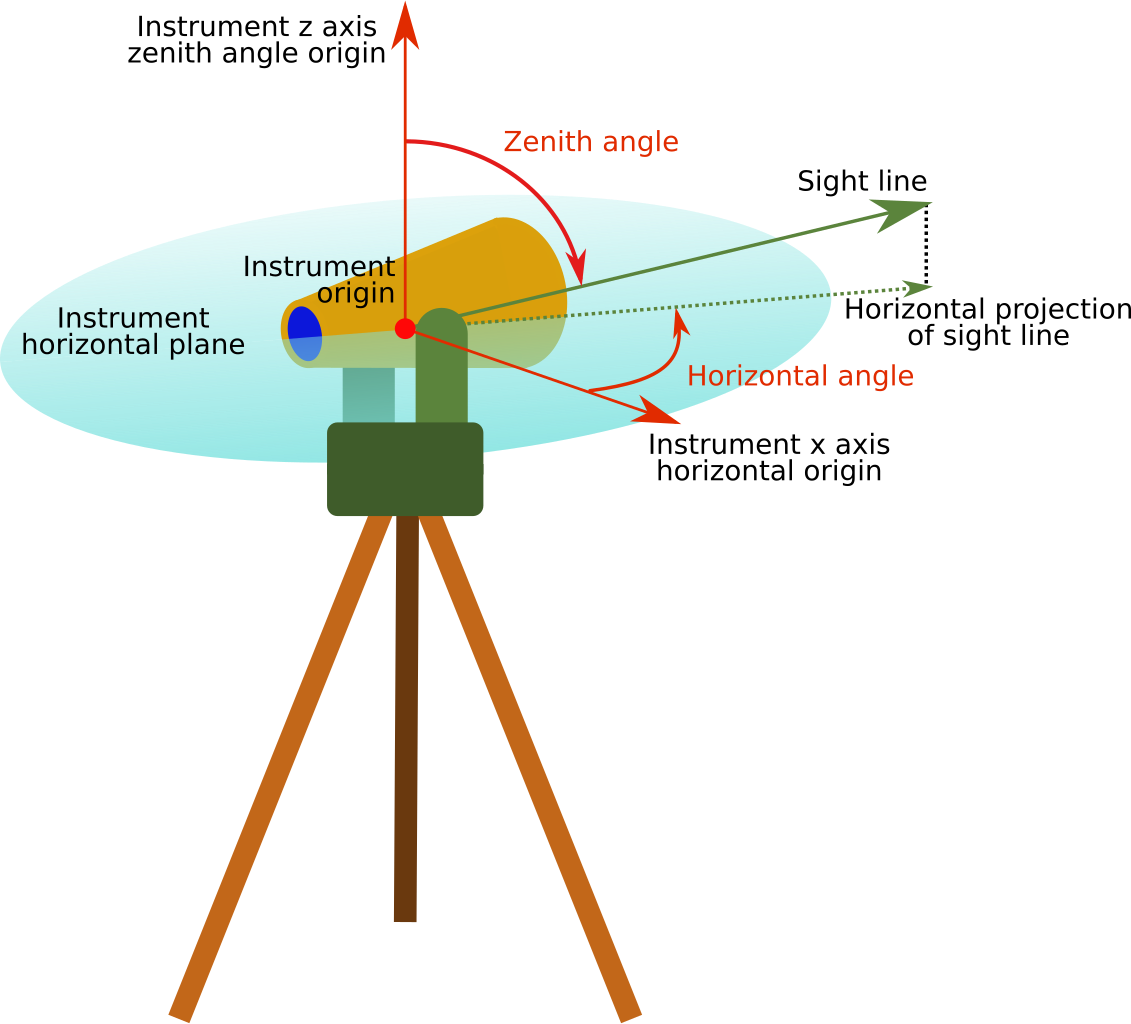
\includegraphics[width=9cm]{CommandReferences/ImagesComRef/topo.png}
\caption{A topo station, its frame and measured angles}
\label{fig:topoStation}
\end{figure}

The following measurements types are currently supported:

\begin{itemize}
    \item distances
    \item horizontal angles
    \item zenithal angles
    \item direct Euclidian vector observation
\end{itemize}

The measurements can be made between cameras poses, GCPs or undeclared points that will be inserted into the last GCP set of the adjustment
(if automatic coordinates initialization succeeds).

Two \CdPPP\ commands can use topo measurements in compensation:
\begin{itemize}
    \item \texttt{OriBundleAdj} via the \texttt{TopoFile} option
    \item \texttt{TopoAdj} (see \ref{subsec:TopoAdj})
\end{itemize}

The topo measurements files can be given as a set of \CdPPP\ json or xml files, or in a simplified text format (named \texttt{OBS} file) inherited from IGN's
Comp3D\footnote{\url{https://github.com/IGNF/Comp3D}} micro-geodesy compensation software.

All the measurements files must be in the \texttt{MMVII-PhgrProj/Topo/[TopoObsName]} folder.

\section{\texttt{OBS} file format}
\label{sec:compObsFormat}

Note: \CdPPP\ supports only a subset of Comp3D \texttt{OBS} format\footnote{\url{https://ignf.github.io/Comp3D/doc/obs.html}}.

\texttt{OBS} files are text files with fields delimited by any number of spaces or tabs. Blank lines are overlooked.
The \texttt{*} character defines a comment that goes up to the end of the line.

A measurement line is composed by:

\begin{itemize}
    \item code: an integer representing the type of observation (see below)
    \item station name
    \item target name
    \item measurement value (in meters for distances, in gon for angles)
    \item measurement \textit{a priori} $\sigma$ (in meters for distances, in gon for angles)
    \item anything else is ignored until the end of the line
\end{itemize}

Example of an \texttt{OBS} line describing a measured distance of 100.0000 m, with a $\sigma$ of 1 mm from \texttt{PointA} to \texttt{PointB}:

\begin{verbatim}
    3   PointA    PointB    100.0000    0.001    * comment
\end{verbatim}

The observations codes are:

\begin{itemize}
    \item \textbf{3}: 3D distance
    \item \textbf{4}: height difference
    \item \textbf{5}: local horizontal (hz) angle
    \item \textbf{6}: local zenithal (zen) angle
    \item \textbf{7}: local horizontal angle for a new station 
    \item \textbf{14}: local $\Delta$x
    \item \textbf{15}: local $\Delta$y
    \item \textbf{16}: local $\Delta$z
\end{itemize}

\newpage
\section{Quickstart example}

An example of topo dataset can be found in \texttt{MMVII/MMVII-UseCaseDataSet/TopoMini/}.
It corresponds to this configuration:

\begin{figure}[!h]
\centering
\includegraphics[width=11cm]{CommandReferences/ImagesComRef/topo2.png}
\caption{The \texttt{TopoMini} dataset}
\label{fig:topoSurvey}
\end{figure}

% PtA and PtD have known coordinates, PtB and PtC coordinates have to be computed (only approximate coordinates are known for this two points).

\subsection{3D points file}
The initial coordinates of the 4 points, in Lambert 93, are in a simple text file (\texttt{inputs/coords.txt}):

\begin{verbatim}
* 1st column:  0 = free point
1  PtA  657700.000  6860700.000  10.000
0  PtB  657710      6860700      10   * approx
0  PtC  657710      6860710      10   * approx
1  PtD  657700.000  6860690.000  10.000
\end{verbatim}

The coordinates of PtA and PtD are supposed known (with a certain precision).
The coordinates of PtB and PtC are just for initialization.
\\

To import these coordinates in \CdPPP\ we use the \texttt{ImportGCP} command, where we give the text format
(additional\_info, name, x, y, z), the name of the resulting \texttt{ObjCoordWorld} and the coordinates SysCo.
We also specify that the points that have '0' for their additional\_info are free points, that the sigma for
known points is 0.001m and that lines starting with '*' are comment lines.

\begin{lstlisting}
MMVII ImportGCP inputs/coords.txt ANXYZ InitL93 ChSys=[L93] AddInfoFree=0 Sigma=0.001 Comment=*
\end{lstlisting}

In the resulting file \texttt{MMVII-PhgrProj/ObjCoordWorld/InitL93/MesGCP-coords.xml},
the points PtA and PtD have a set \texttt{\_\_Opt\_\_Sigma2} equivalent to $\sigma = 0.001 m$ ,
the points PtB and PtC have no \texttt{\_\_Opt\_\_Sigma2}, making them free points.


\subsection{SysCo}

A \texttt{RTL} SysCo is mandatory to be able to compute a topo compensation.
PtA is chosen as RTL origin (tangency point).
The SysCo definition according to \ref{subsec:SysCoDef} is: \texttt{RTL*657700*6860700*0*IGNF:LAMB93}.
The \texttt{GCPChSysCo} command does the conversion to \texttt{RTL}:

\begin{lstlisting}
MMVII GCPChSysCo "RTL*657700*6860700*0*IGNF:LAMB93" InitL93 InitRTL
\end{lstlisting}


The two previous steps can be done in one \texttt{ImportGCP} call, the \texttt{ChSys} parameter accepting two
SysCos:

\begin{lstlisting}
MMVII ImportGCP inputs/coords.txt ANXYZ InitL93 ChSys="[L93,RTL*657700*6860700*0*IGNF:LAMB93]" AddInfoFree=0 Sigma=0.001 Comment=*
\end{lstlisting}

\subsection{Auto RTL SysCo}

\texttt{ImportGCP} can automatically create a \texttt{RTL} SysCo, with its origin equal to the average of the input coordinates:
just give \texttt{RTL} as the destination SysCo. This new SysCo will be saved as \texttt{MMVII-PhgrProj/SysCo/RTL.xml}, making
the SysCo available for every following command as \texttt{RTL}.

\begin{lstlisting}
MMVII ImportGCP inputs/coords.txt ANXYZ InitL93 ChSys=[L93,RTL] AddInfoFree=0 Sigma=0.001 Comment=*
\end{lstlisting}

\begin{comment}
\subsection{SysCo shortcut}
The SysCo file \texttt{MMVII-PhgrProj/ObjCoordWorld/InitRTL/CurSysCo.xml}, created by \texttt{ImportGCP}
can be used to create a shortcut name for \texttt{RTL*657700*6860700*0*IGNF:LAMB93}.

We just have to copy it as \texttt{MMVII-PhgrProj/SysCo/RTL.xml} to be able to designate this SysCo
simply as \texttt{RTL} for the rest of the example.

\begin{lstlisting}
cp MMVII-PhgrProj/ObjCoordWorld/InitRTL/CurSysCo.xml MMVII-PhgrProj/SysCo/RTL.xml
\end{lstlisting}
\end{comment}


\subsection{Measurements}
The measurements are:
\begin{itemize}
   \item an instrument on PtA measures hz angle, zen angle and distance to PtB and PtC
   \item an instrument on PtD measures hz angle, zen angle and distance to PtB and PtC
\end{itemize}
The corresponding \texttt{OBS} file (\texttt{inputs/meas.obs}) is:
\begin{verbatim}
 7   PtA    PtB     0      0.001
 6   PtA    PtB   100      0.001
 3   PtA    PtB    10.05   0.005
 5   PtA    PtC   -40.62   0.001
 6   PtA    PtC   100      0.001
 3   PtA    PtC    14.88   0.005

 7   PtD    PtB     0      0.001
 6   PtD    PtB   100      0.001
 3   PtD    PtB    14.88   0.005
 5   PtD    PtC   -14.96   0.001
 6   PtD    PtC   100      0.001
 3   PtD    PtC    22.82   0.005
\end{verbatim}
This file has to be put into a subdirectory of \texttt{MMVII-PhgrProj/Topo} via the \texttt{ImportOBS} command:
\begin{lstlisting}
MMVII ImportOBS inputs/meas.obs Obs1
\end{lstlisting}


\subsection{Unknowns count}

The previous \texttt{OBS} file creates two verticalized stations, one with its origin on PtA, the other on PtD.
Each of these stations has an horizontal orientation unknown ($G_0$) due to the random orientation of the instrument
when it has been set on the point.

The number of unknowns in this configuration is:
\begin{itemize}
   \item 3 per point ($x, y, z$)  $\rightarrow$ \textit{12 unknowns}
   \item 1 per station ($G_0$)  $\rightarrow$ \textit{2 unknowns}
\end{itemize}

Which gives a total of 14 unknowns for the 4 points and 2 stations.
% Total: $4 \times 3 + 2 \times 1 = 14$ unknowns.
\\

The number of constraints is:
\begin{itemize}
   \item 3 per constrained point, PtA and PtD  $\rightarrow$ \textit{6 constraints}
   \item 1 per topo measurement $\rightarrow$ \textit{12 constraints}
\end{itemize}

Which gives a total of 18 constraints.
% Total: $2 \times 3 + 12 = 18$ constraints.


\subsection{Adjustment}
\label{subsec:TopoAdj}
The \texttt{TopoAdj} command can perform an adjustment between topo and GCP constraints.
It is used as a substitute to \texttt{OriBundleAdj} when there are no cameras.

\begin{verbatim}
 == Mandatory unnamed args : ==
  * string [Topo,In] :: Dir for Topo measures
  * string [Topo,Out] :: Dir for Topo measures output
  * std::vector<std::vector<std::string>> :: GCP ground coords and sigma factor,
                        SG=0 fix, SG<0 schurr elim, SG>0
                        and optional output dir [[Folder,SigG,FOut?],...]]

 == Optional named args : ==
  * [Name=DataDir] string :: Default data directories  ,[Default=Std]
  * [Name=NbIter] int :: Number of iterations ,[Default=10]
  * [Name=GCPFilter] string :: Pattern to filter GCP by name
  * [Name=GCPFilterAdd] string :: Pattern to filter GCP by additional info
  * [Name=LVM] double :: Levenberg–Marquardt parameter (to have better conditioning
                        of least squares) ,[Default=0]
\end{verbatim}

In our example, the input topo directory is \texttt{Obs1} and the input ObjCoordWorld is \texttt{InitRTL}.
We give output directories names for topo and points.
\begin{lstlisting}
MMVII TopoAdj Obs1 Obs1_out [[InitRTL,1,FinalRTL]]
\end{lstlisting}

The final $\sigma_0$ value should be around 1 if everything goes well.
In this example, $\sigma_{0 init} > 5000$, because the initial coordinates of PtB and PtC are approximate,
and after 10 iterations it stabilizes at $\sigma_{0 final} = 1.7$.
\\

The output topo directory contains a single xml file with all the measurements and some output values (residuals,
stations orientations...). It can be used as topo input file.
\\

The last step is to convert the RTL coordinates to Lambert 93:

\begin{lstlisting}
MMVII GCPChSysCo L93 FinalRTL FinalL93
\end{lstlisting}


\section{Stations orientation constraints}

Each station has orientation constraints that have to be given before the station observations lines in the \texttt{OBS} file.
Each orientation constraint is indicated as a line starting with \texttt{\#} (from now on, called a \texttt{\#}-line).
\\

The possible orientation constraints are:
\begin{itemize}
   \item \texttt{\#FIX}: the station is axis-aligned, it is verticalized and oriented to North
   \item \texttt{\#VERT}: the station is verticalized and only horizontal orientation is free
   \item \texttt{\#BASC}: the station orientation has 3 degrees of freedom, meaning non-verticalized and not oriented to North
   \item TODO \texttt{\#CAM}:the station orientation is the camera orientation (only allowed for point names that correspond to image file names)
\end{itemize}

After a \texttt{\#}-line, all the following stations have the new orientation constraint until the next \texttt{\#}-line with new orientation unknowns.
For convenience, \texttt{\#NEW} can be used to keep current orientation constraint type and just add new unknowns for orientation (see \ref{subsec:SeveralStationsSamePoint}).


Each \texttt{OBS} file starts with an implicit \texttt{\#VERT}, making the stations verticalized by default.

For now, the vertical is modeled as the Earth's ellipsoid normal. Vertical deflection grids may be added later.



\subsection{Frames for survey stations}

The computation must take place in a 3D euclidian frame. For now, only RTL SysCo is supported.
Figure \ref{fig:topoFrames} shows the frames used in topo compensation.

\begin{figure}[!h]
\centering
\includegraphics[width=12cm]{Programmer/framesTopo.png}
\caption{The different frames types used in compensation:
   \texttt{Green}: a projection SysCo. As it is not euclidian, compensation should not be done in this frame.
   \texttt{Blue}: the RTL SysCo for the computation. Every parameter is in this frame.
   \texttt{Purple}: each 3D point has its own local euclidian frame tangent to the ellipsoid.
   \texttt{Yellow}: each topometric station has a rotation between the local euclidian tangent frame and the instrument frame.
 }
\label{fig:topoFrames}
\end{figure}


Stations orientation constraints fix some parts of the rotation between local tangent frame and instrument frame:
no rotation (\textbf{\#FIX}), rotation around $Z$ only (\textbf{\#VERT}), or free rotation (\textbf{\#BASC}).



\subsection{Return to quickstart example}
The example \texttt{OBS} file was:
\begin{verbatim}
 7   PtA    PtB     0      0.001
 6   PtA    PtB   100      0.001
 3   PtA    PtB    10.05   0.005
 5   PtA    PtC   -40.62   0.001
 6   PtA    PtC   100      0.001
 3   PtA    PtC    14.88   0.005

 7   PtD    PtB     0      0.001
 6   PtD    PtB   100      0.001
 3   PtD    PtB    14.88   0.005
 5   PtD    PtC   -14.96   0.001
 6   PtD    PtC   100      0.001
 3   PtD    PtC    22.82   0.005
\end{verbatim}

It is possible to say that the station on PtA was not verticalized by using \texttt{\#BASC}:
\begin{verbatim}
#BASC
 7   PtA    PtB     0      0.001
 6   PtA    PtB   100      0.001
 3   PtA    PtB    10.05   0.005
 5   PtA    PtC   -40.62   0.001
 6   PtA    PtC   100      0.001
 3   PtA    PtC    14.88   0.005

#VERT
 7   PtD    PtB     0      0.001
 6   PtD    PtB   100      0.001
 3   PtD    PtB    14.88   0.005
 5   PtD    PtC   -14.96   0.001
 6   PtD    PtC   100      0.001
 3   PtD    PtC    22.82   0.005
\end{verbatim}

This will free the 3D rotation of the station on PtA, adding two rotations unknowns to the computation.
\newline

It is also possible to use \texttt{\#FIX} to remove the horizontal orientation unknown $G_0$ of a station, expressing the fact that it
is verticalized and the horizontal reference is North:
\begin{verbatim}
#FIX
 7   PtA    PtB     0      0.001
 6   PtA    PtB   100      0.001
 3   PtA    PtB    10.05   0.005
 5   PtA    PtC   -40.62   0.001
 6   PtA    PtC   100      0.001
 3   PtA    PtC    14.88   0.005

#VERT
 7   PtD    PtB     0      0.001
 6   PtD    PtB   100      0.001
 3   PtD    PtB    14.88   0.005
 5   PtD    PtC   -14.96   0.001
 6   PtD    PtC   100      0.001
 3   PtD    PtC    22.82   0.005
\end{verbatim}


\subsection{Several stations on the same point}
\label{subsec:SeveralStationsSamePoint}

\CdPPP\ automatically creates a new station when a point is used for the first time as the origin of a measurement.

If we have to make a new set of orientation unknowns because two instruments were set on the same point with different
orientations, we can either:

\begin{itemize}
   \item use separate \texttt{OBS} files
   \item add a \texttt{\#}-line to separate the measurements sets (\texttt{\#NEW} is useful in this case to make a station with the same orientation constraints as before)
   \item use a code \textbf{7} instead of \textbf{5} for the first measurement of the new station
\end{itemize}

A separate \texttt{OBS} files or a \texttt{\#}-line closes all current stations.
Code \textbf{7} only closes the previous station on one point. 

Some illustrations :
\begin{verbatim}
 7   St1    PtA   100.000   0.001 * creates a station on St1
 5   St1    PtB   110.000   0.001

 7   St1    PtA   150.000   0.001 * closes current station on St1, creates a new one on St1
 5   St1    PtC   210.000   0.001
\end{verbatim}
Creates two stations originating on point \texttt{St1}. Each of these station
is vericalized (thanks to the implicit \texttt{\#VERT} at the start of the file) and each has one horizontal orientation unknown.
Here, there is a 50 grades difference between the two stations orientations.

With:
\begin{verbatim}
 7   St1    PtA     100.000      0.001 * creates a station on St1
 5   St1    PtB     110.000      0.001

 5   St1    PtA     150.000      0.001
 5   St1    PtC     210.000      0.001
\end{verbatim}
There is only one station on \texttt{St1}. The incoherent horizontal angles values
will make the computation fail.

Another way to fix it:
\begin{verbatim}
 5   St1    PtA     100.000      0.001 * creates a station on St1
 5   St1    PtB     110.000      0.001
#NEW                                   * closes all current stations
 5   St1    PtA     150.000      0.001 * creates a station on St1
 5   St1    PtC     210.000      0.001
\end{verbatim}
The fisrt \textbf{7} is not mandatory since it is the start of a file, there is no
current stations. \texttt{\#NEW} closes all the current stations, keeping the same orientations constraints (stations verticalized).

Code \textbf{7} only closes the current station on one point :
\begin{verbatim}
 5   St1    PtA   100.000   0.001 * creates a station on St1
 5   St1    PtB   110.000   0.001
 
 5   St2    PtA   200.000   0.001 * creates a station on St2
 5   St2    PtD   300.000   0.001

 7   St1    PtA   150.000   0.001 * closes station on St1, creates a new one on St1
 5   St1    PtC   210.000   0.001

 5   St2    PtE   250.000   0.001 * uses previous station on St2
\end{verbatim}
But:
\begin{verbatim}
 5   St1    PtA   100.000   0.001 * creates a station on St1
 5   St1    PtB   110.000   0.001
 
 5   St2    PtA   200.000   0.001 * creates a station on St2
 5   St2    PtD   300.000   0.001
#NEW                              * closes all the stations
 5   St1    PtA   150.000   0.001 * creates a station on St1
 5   St1    PtC   210.000   0.001

 5   St2    PtE   250.000   0.001 * creates a station on St2
\end{verbatim}


\subsection{Special case for distance-only measurements}

If a station only has distances measurements, it is automatically
set as a \texttt{\#FIX} station, since this station orientation unknowns
can't be estimated.


\section{Topo measurements for minimal external constraints}

For any kind of adjustment, minimal constraints can be useful to get the measurements internal precision.
In general, several GCP with known coordinates are used to fix the frame, but their inconsistency may
impact the computation.

In a 3D adjustment, up to 7 external constraints have to be provided to fix the frame translation, rotation ($R_X$, $R_Y$, $R_Z$) and scale.

With photogrammetry, one camera pose can be used to fix 6 external constraints. The scale can then be given with an \texttt{OBS} file:
\begin{verbatim}
    * distance of 10 meters between IMG1.JPG and IMG2.JPG poses centers
    3  IMG1.JPG  IMG2.JPG 10.0000 0.0010   
\end{verbatim}

Another possibility is to constrain the coordinates of one GCP, then add an \texttt{OBS} file to fix the scale and the 3 rotations:
\begin{verbatim}
    3  IMG1.JPG  IMG2.JPG 10.0000 0.0010   * scale constraint

    #FIX  * do not add a rotation unknown
    5  IMG1.JPG  GCP_10  0   0.0010   * GCP_10 is north from IMG1.JPG => constraints Rz

    * two Za=Zb constraints between non-aligned points to constrain Rx and Ry
    16  GCP_03  GCP_10  0 0.0010
    16  GCP_03  GCP_11  0 0.0010
\end{verbatim}

Minimal external constraints for the quickstart example means having constraints on only one point and this \texttt{OBS} file:

\begin{verbatim}
#FIX
 5   PtA    PtB   100      0.001 * PtA => PtB = East. Code 7 or 5 are equivalent here
 
#VERT
 7   PtA    PtB     0      0.001
 6   PtA    PtB   100      0.001
 3   PtA    PtB    10.05   0.005
 5   PtA    PtC   -40.62   0.001
 6   PtA    PtC   100      0.001
 3   PtA    PtC    14.88   0.005

 7   PtD    PtB     0      0.001
 6   PtD    PtB   100      0.001
 3   PtD    PtB    14.88   0.005
 5   PtD    PtC   -14.96   0.001
 6   PtD    PtC   100      0.001
 3   PtD    PtC    22.82   0.005
\end{verbatim}


\begin{comment}
\section{Topometric adjustment example}
\label{subsec:topoBench}

The example is used in \texttt{TopoComp} Bench. It is created by the method \texttt{cTopoData::createEx1()}.
We will describe the input files equivalent for the \texttt{TopoAdj} command.


\subsection{Creating the points}

The points with their initial coordinates and the sigmas on their coordinates constraints
are given in a GCP file. 

3 points have coordinates constraints at 1 cm ($A$, $B$, $C$). They form an isosceles triangle
on an horizontal plane.
A 4th point ($D$) is declared above the other. It has no \texttt{\_\_Opt\_\_Sigma2} attribute in the GCP file as this point is free.
(Fig. \ref{fig:topoEx1}). Note that depending on the initial coordinates for $D$, the computation may no succeed
(i.e., if $A$ and $D$ have the same initial coordinates, the distance formula derivatives are $NaN$).

A \texttt{CurSysCo.xml} must come along this GCP file to describe the RTL SysCo.


\begin{figure}[!h]
\centering
\includegraphics[width=12cm]{Programmer/benchtopo1b.png}
\caption{The 3 fixed points ($A$, $B$, $C$) and the free point ($D$)}
\label{fig:topoEx1}
\end{figure}

The summarized content of the GCP file:

\begin{lstlisting}
      <SetGCP>
         <NameSet>"terrain"</NameSet>
         <Measures>
            <el>
               <Name>"A"</Name>
               <Pt>10 10 10</Pt>
               <AdditionalInfo>""</AdditionalInfo>
               <__Opt__Sigma2>.0001 0 0 .0001 0 .0001</__Opt__Sigma2>
            </el>
            <el>
               <Name>"B"</Name>
               <Pt>20 10 10</Pt>
               <AdditionalInfo>""</AdditionalInfo>
               <__Opt__Sigma2>.0001 0 0 .0001 0 .0001</__Opt__Sigma2>
            </el>
            <el>
               <Name>"C"</Name>
               <Pt>15 20 10</Pt>
               <AdditionalInfo>""</AdditionalInfo>
               <__Opt__Sigma2>.0001 0 0 .0001 0 .0001</__Opt__Sigma2>
            </el>
            <el>
               <Name>"D"</Name>
               <Pt>14 14 14</Pt>
               <AdditionalInfo>""</AdditionalInfo>
            </el>
         </Measures>
      </SetGCP>
\end{lstlisting}


\subsection{Creating the observations}

The distances from $D$ to $A$, $B$ and $C$ are measured. For redundancy and error evaluation, the distance from $D$ to $C$ is measured twice
with different values (Fig. \ref{fig:topoEx2}).

\begin{figure}[!h]
\centering
\includegraphics[width=12cm]{Programmer/benchtopo2.png}
\caption{Point $D$ is determined by measured distances}
\label{fig:topoEx2}
\end{figure}

Observations are represented in an \texttt{OBS} file:
\begin{lstlisting}
    3  D  A  10.0  0.1
    3  D  B  10.0  0.1
    3  D  C  10.0  0.1
    3  D  C  10.1  0.1
\end{lstlisting}

Here a implicit station is created, based on point $D$.
As no orientation status is given, the station is supposed verticalized.
It should have an horizontal orientation degree of liberty.
But since there is no observations able to determine the station orientation,
it is automatically set as fixed (as if a \texttt{\#FIX} line was added at the start of the file).

\subsection{Outputs}

After a computation, the output GCP file contains the final coordinates of every point, including
points that were not declared in the input GCP, but referenced in the topo measurements.

The output Topo file contains info about all the stations and observations,
with output values as residuals:

\begin{lstlisting}
<TopoData>
 <AllObsSetStations>
    <el>
       <TopoObsSetData>
          <Type>"Station"</Type>
          <AllObs>
             <el>
                <TopoObsData>
                   <Type>"Dist"</Type>
                   <Pts>    <el>"D"</el>     <el>"A"</el>       </Pts>
                   <Measures>    <el>10</el>      </Measures>
                   <Sigmas>   <el>0.1</el>     </Sigmas>
                   <__Opt__LastResiduals>  <el>-0.000000000000002</el>  </__Opt__LastResiduals>
                </TopoObsData>
             </el>
[...]
             <el>
                <TopoObsData>
                   <Type>"Dist"</Type>
                   <Pts>      <el>"D"</el>     <el>"C"</el>          </Pts>
                   <Measures>     <el>10.1</el>         </Measures>
                   <Sigmas>       <el>0.1</el>           </Sigmas>
                   <__Opt__LastResiduals>  <el>-0.050000000000001</el>  </__Opt__LastResiduals>
                </TopoObsData>
             </el>
          </AllObs>
          <StationOriStatus>"#FIX"</StationOriStatus>
          <__Opt__Out_G0>0</__Opt__Out_G0>
       </TopoObsSetData>
    </el>
 </AllObsSetStations>
</TopoData>
\end{lstlisting}

This Topo file can be used as input for another adjustment (it is completely equivalent to the \texttt{OBS} file).

\end{comment}



%###########################################################################################################
%###########################################################################################################
%-------------------------------------------- TUTORIAM -----------------------------------------------------
%###########################################################################################################
%###########################################################################################################

\part{Tutorial and exercises}

\include{Tutorial/TutoOrient}

%   ------------------------------------------------------------------
%   ------------------------------------------------------------------
%                 Chapter set editing
%   ------------------------------------------------------------------
%   ------------------------------------------------------------------

\chapter{Use cases}

In all this use cases, the folder contains a file {\tt Info.txt} tha contains a list of
all commands plus some brief commentary.

%   ------------------------------------------------------------------
%   ------------------------------------------------------------------
%   ------------------------------------------------------------------

\section{Image devlopment}

%   ------------------------------------------------------------------
\subsection{Introduction/presentation}

This data set present a use-case for creation a devloped surface.  A detailled
description of the MMVII-command can be found in chapter~\ref{Chap:Mesh}.
The data, located in folder {\tt DevlopImage}  is made of $74$ images that correspond to a stereoscopic
acquisition of a map that present high, but smooth, deformation.


For the purpose of limitating the size in github, the images have been articifially
reduced of a factor $4$. Also the image have been made in non professional
condition with natural ligthing. Globally, the quality of the result is
not representative of what can be obtained by such tools.

A file {\tt Info.txt} contains the list of all command used, somes are in
comment.
At several step of the process, the pipeline requires some input of the user
(for example $2d$ and $3d$ masq).  To assure the reproductability, the 
data set provide a copy of the input that was made in floder {\tt DataAux}. 
In this case, in the file {\tt Info.txt}  the interactive command is commented, and subsitued
by a shell command that copy the data, for example :

\begin{itemize}
    \item for seizing the $3d$ masq, the command {\tt"mm3d SaisieMasqQT AperiCloud\_Basc.ply"}
	    is indicated but commented;
    \item to execute the process, the command {\tt "cp DataAux/AperiCloud\_Basc\_* ."} is indicated.
\end{itemize}

At this step, the pipeline is a mix of {\tt mmv1} and {\tt MMVII}. We give a fast description
of the {\tt mmv1} part as it is a classical pipeline and let the reader find more details
in the $500$ pages of the  {\tt mmv1} documentation.


%   ------------------------------------------------------------------

\subsection{The  {\tt mmv1} part}

The  {\tt mmv1} goes until the obtention of $3d$ mesh that describe the surfaces and
pose estimation of camera in the same repair.

     %   -  -  -  -  -  -  -  -  -  -  -  -  -  -  -  -  -  -  -  -  -  -  -  -

\subsubsection{Camera pose and calibration}

As the reduction has supressed the {\tt xif} meta-data, we indicate it
for {\tt mmv1}, the folder contains a file :

\begin{itemize}
    \item {\tt MicMac-LocalChantierDescripteur.xml}
\end{itemize}

We compute tie-point using {\tt @SFS} because of low contrast :

\begin{itemize}
    \item {\tt mm3d Tapioca MulScale ".*jpg" 400 1500 @SFS}
\end{itemize}

We compute orientation and calibration : 

\begin{itemize}
   \item {\tt Tapas FraserBasic "P.*jpg" Out=AllRel}
\end{itemize}

For  this pipeline, it's not absolutely necessary to be in a physicall repair,
but that's a good use to have ... We can seize the information with
{\tt SaisieBasc} and {\tt SaisieMasqQT}, replaced here by {\tt cp} from {\tt DataAux} . 
Once done we use :

\begin{itemize}
    \item {\tt mm3d SBGlobBascule P.*jpg Ori-AllRel/ MesBasc-S2D.xml Basc  PostPlan=Plan DistFS=10}
\end{itemize}

     %   -  -  -  -  -  -  -  -  -  -  -  -  -  -  -  -  -  -  -  -  -  -  -  -

\subsubsection{Computation of $3d$ model}

We must first create a $3d$ masq of the zone that will be used at different step .
We first create a sparse cloud for seizing :

\begin{itemize}
	\item {\tt AperiCloud "P.*jpg" Ori-Basc/}
\end{itemize}

After we can use {\tt mm3d SaisieMasqQT AperiCloud\_Basc.ply}, 
replaced here by a {\tt cp} from {\tt DataAux}.
Then we compute the $3D$ dense cloud :

\begin{itemize}
	\item {\tt mm3d C3DC BigMac P.*jpg Ori-Basc/ Masq3D=AperiCloud\_Basc\_selectionInfo.xml}
\end{itemize}

Finaly, we transform it in a $3d$ mesh :

\begin{itemize}
	\item {\tt TiPunch C3DC\_BigMac.ply Filter=0}
\end{itemize}

%   ------------------------------------------------------------------

\subsection{The  {\tt MMVII} part}

     %   -  -  -  -  -  -  -  -  -  -  -  -  -  -  -  -  -  -  -  -  -  -  -  -

\subsubsection{Inporting the data}

In the {\tt MMVII} part we need the pose of camera and the $3D$ mesh. The $3d$ mesh is 
in the standard  {\tt ply} format that is supported by  {\tt MMVII}, so there is nothing
to do. For the importing the orientation  we can use :

\begin{itemize}
	\item {\tt MVII OriConvV1V2 Ori-Basc/ Basc}
\end{itemize}

Curious reader, can inspect the folder {\tt MMVII-PhgrProj/Ori/Basc/}.

     %   -  -  -  -  -  -  -  -  -  -  -  -  -  -  -  -  -  -  -  -  -  -  -  -

\subsubsection{Correcting and filtering the mesh}

We use the command {\tt MeshCheck} and {\tt MeshCloudClip}, the first one
correct some topologicall probleme in the mesh, the second one restric
the mesh to our usefull zone  (because the poisson algorithm used in {\tt TiPunch}
create undesirable extensions) :

\begin{itemize}
	\item {\tt MMVII  MeshCheck C3DC\_BigMac\_mesh.ply Out=Correc-C3DC\_BigMac\_mesh.ply Bin=1}

	\item {\tt MMVII  MeshCloudClip Correc-C3DC\_BigMac\_mesh.ply  AperiCloud\_Basc\_polyg3d.xml}
\end{itemize}

     %   -  -  -  -  -  -  -  -  -  -  -  -  -  -  -  -  -  -  -  -  -  -  -  -

\subsubsection{Devlopment of the mesh}

Now we run the "kernel" algorithm to create the $2d$ development of the mesh :

\begin{lstlisting}
MMVII MeshDev Clip\_Correc-C3DC\_BigMac\_mesh.ply 
\end{lstlisting}

This command generate $2$ mesh :

\begin{itemize}
	\item {\tt Dev2D\_Clip\_Correc-C3DC\_BigMac\_mesh.ply} which is the devlopped surface itself,
              if may contain less triangle/point that the $3d$ intial mesh when this one is badly connected 
		
	\item {\tt Dev3D\_Clip\_Correc-C3DC\_BigMac\_mesh.ply} which is a subset of the $3D$ initial mesh
		that correpond to the $2D$ devlopped mesh (it will be equal to initial when there is no connectivity problem);
\end{itemize}

     %   -  -  -  -  -  -  -  -  -  -  -  -  -  -  -  -  -  -  -  -  -  -  -  -

\subsubsection{Computing visibility, quality , radiometry of triangles}

We now run the command  {\tt MeshProjImage} to prepare the texture mapping : this command
compute the visibility of each triangle in each image, it also computes tie points with 
radiometry to compute radiometric equalisation 

\begin{itemize}
    \item {\tt MMVII MeshProjImage "P.*jpg"  Dev3D\_Clip\_Correc-C3DC\_BigMac\_mesh.ply Basc DEV OutRadData=R0}
\end{itemize}

The parameter {\tt DEV} indicates where the data must be stored.
The parameter {\tt OutRad=R0} indicate that data for radiometry 
must be compute, and fix the folder where these data must be stored.

     %   -  -  -  -  -  -  -  -  -  -  -  -  -  -  -  -  -  -  -  -  -  -  -  -

\subsubsection{Equalizing the radiometry}

For radiometric equalization, we must know the aperture used for each image,
as the vignettage is dependand of aperture. As these images contains no metadata,
we must indicate it . This has to be indicated in the file :

\begin{itemize}
    \item {\tt MMVII-PhgrProj/MetaData/Std/CalcMTD.xml}
\end{itemize}

We can do it by copying the file {\tt DataAux/CalcMTD.xml}. We can also
do it using the command {\tt EditCalcMTDI} :

\begin{itemize}
      \item {\tt MMVII  EditCalcMTDI Std Aperture "Modif=[P.*.jpg,11,0]"  Save=1}
\end{itemize}

We must first create the initial radiometric model  we want to use, here we select
a degree $2$ by image :

\begin{itemize}
	\item {\tt MMVII RadiomCreateModel P.*jpg Init2 Basc DegIma=2}
\end{itemize}

Now we can compute the radometric equalization model :

\begin{itemize}
	\item {\tt MMVII RadiomComputeEqual P.*jpg R0 Init2 Equal Basc}
\end{itemize}


     %   -  -  -  -  -  -  -  -  -  -  -  -  -  -  -  -  -  -  -  -  -  -  -  -

\subsubsection{Map the texture}

And finally, we can create the devloped surface :


\begin{itemize}
	\item {\tt MMVII MeshImageDevlp Dev2D\_Clip\_Correc-C3DC\_BigMac\_mesh.ply  DEV InRadModel=Equal}
\end{itemize}

The results can be found in {\tt MMVII-PhgrProj/MeshDev/DEV/DevIm.tif}, an illustration is shown on figure~\ref{fig:TutDI:DevIm}.


\begin{figure}
\centering
	\includegraphics[width=12 cm]{Tutorial/Images/DevIm.jpg}
	\caption{Example of devloped image}
\label{fig:TutDI:DevIm}
\end{figure}



%   ------------------------------------------------------------------
%   ------------------------------------------------------------------
%   ------------------------------------------------------------------

\section{Coded target processing}

%   ------------------------------------------------------------------

\subsection{Introduction/presentation}

This data set, located on {\tt Circ-Code-Target} is representative of an acquisition specially made for close 
range calibration of a camera, or block rigid camera.  The images have been
acquired on specially build camera panel ; the caracteristics of this panel
is the following (see an example on figure~\ref{fig:CodeT:Panel}) :
 

\begin{itemize}
     \item it contain arround $234$ targets, which $3d$ position has been accurately measured;

     \item arround $\frac{1}{4}$ of these targets are coded target that allow a firt full automatic pipeline,
           while the non coded target can  be automatically matched in a second iteration;

     \item for easiness of conception,  the majority of the points are in a plane, by the way $3$ target
           are outside the plane  to offer a better calibration of the focal length;
\end{itemize}


\begin{figure}
\centering
	\includegraphics[width=5cm]{Tutorial/Images/Perche.jpg}
	\caption{An extract of panel including the $3$ foreground target.}
\label{fig:CodeT:Panel}
\end{figure}


The acquisition system initially contain $4$ camera in a rigid block position, each camera acquired
$40$ images of $6000 \times  4000$ pixels. For limiting the size of data on github, the following reduction
where applied : limitation to $2$ camera, $20$ images per camera and downsizing the image to $2000 \times  1333$ pixels

The images contain no meta-data, but we "know" that :

\begin{itemize}
     \item the camera model is a Nikon D5600 ;
     \item the focal lenght is a $24mm$, in equivalent $35mm$ (in fact a $16mm$);
     \item different instance of the same camera have been used in the rigid
           block, the $3$ first digit of image name can be used as identifier
           (i.e. two images have been acquired with the same camera iff their name have the
		same $3$ first digit);
\end{itemize}


%   ------------------------------------------------------------------

\subsection{Extract the target in image}

     %   -  -  -  -  -  -  -  -  -  -  -  -  -  -  -  -  -  -  -  -  -  -  -  -

\subsubsection{Create specification}

{\tt MMVII} offers a flexible way to specify coding system (see \ref{GenEncodS}) :
number of bits, redundancy,  maximal run, geometry ... By the way, here we use
an existing system, so we have no flexibility and just have to specify the reference 
of this system.  Using the general formalism, we do it in two steps, first generate
the encoding, i.e. the set of bit-vector :

\begin{lstlisting}
MMVII  CodedTargetGenerateEncoding CERN 14
\end{lstlisting}

The command generate a file {\tt CERN\_Nbb14\_Freq14\_Hamm1\_Run1000\_1000\_SpecEncoding.xml}
that contains the list of code used. An extract :

\begin{lstlisting}
...
     <el>  <!--10110001000000-->
            <NumCode>4 141</NumCode>
            <Name>"004"</Name>
     </el>
...
\end{lstlisting}

A quick command on the file :

\begin{itemize}
	\item the vector of bit, on $14$ bits  {\tt "10110001000000"} is indicated
		as  commentary (only for ;
        \item it correspond to$128+8+4+1=141$, this is $141$ which is saved
		and used by {\tt MMVII} to compute the bit vvect
	\item  the  number $4$ will be used as identifier  (it's the number printed on the targets);
	\item  the  name {\tt "004"} is the string version.
\end{itemize}

After we generate a file that contains the complete specification : the coding itself
\emph{and} the aspect of the target : geometry and radiometry .  Here again
as we use an existing external system, we dont change anything to default parameters.

\begin{lstlisting}
MMVII  CodedTargetGenerate  CERN_Nbb14_Freq14_Hamm1_Run1000_1000_SpecEncoding.xml
\end{lstlisting}

In case we want to generate an image of the targets (for printing them) we can
use the optionnal parameter {\tt PatIm}.

\begin{lstlisting}
MMVII  CodedTargetGenerate  CERN_Nbb14_Freq14_Hamm1_Run1000_1000_SpecEncoding.xml  PatIm=001
\end{lstlisting}

     %   -  -  -  -  -  -  -  -  -  -  -  -  -  -  -  -  -  -  -  -  -  -  -  -

\subsubsection{Extract the target}

We can now run the extraction of target in image :

\begin{lstlisting}
MMVII  CodedTargetCircExtract 043_0005_Scaled.tif CERN_Nbb14_Freq14_Hamm1_Run1000_1000_FullSpecif.xml DiamMin=8
\end{lstlisting}

Note the parameter {\tt DiamMin=8} necessary here because downscaling has created relatively small targets. 
The result are written in a subfolder of {\tt MMVII-PhgrProj/PointsMeasure/}, by default it's the subfolder
{\tt Std/}, that contains now $2$ files :

\begin{itemize}
	\item {\tt MesIm-043\_0005\_Scaled.tif.xml} that contains the position of the targets, used in standard process;
	\item {\tt Attribute-MesIm-043\_0005\_Scaled.tif.xml} that contains the geometry of ellipses (used in completion/refinement);
\end{itemize}


If we want to check the result we can add the parameter {\tt VisuEllipse=1} to generate an image
including the exracted coded and uncoded targets :


\begin{lstlisting}
MMVII  CodedTargetCircExtract 043_0005_Scaled.tif CERN_Nbb14_Freq14_Hamm1_Run1000_1000_FullSpecif.xml  DiamMin=8 VisuEllipse=1
\end{lstlisting}

An example of result is shown on figure~\ref{fig:CodeT:Panel}.

\begin{figure}
\centering
	\includegraphics[width=12 cm]{Tutorial/Images/VisuEllips.jpg}
	\caption{An example of the visualization generated}
\label{fig:CodeT:Panel}
\end{figure}

It's possible, to change the destination of result using parameter {\tt OutPointsMeasure}.
Using pattern, its possible to run the research on all the image of the dataset, computation will be parelized .
Like every command {\tt MMVII}, it's possible to restrict the number of processor using the optionnal parameter
{\tt NbProc} :

\begin{lstlisting}
MMVII  CodedTargetCircExtract ".*_Scaled.tif" CERN_Nbb14_Freq14_Hamm1_Run1000_1000_FullSpecif.xml DiamMin=8 NbProc=2 OutPointsMeasure=Test
\end{lstlisting}


%   ------------------------------------------------------------------

\subsection{Estimate pose and calibration simultenaously}

     %   -  -  -  -  -  -  -  -  -  -  -  -  -  -  -  -  -  -  -  -  -  -  -  -

\subsubsection{For one camera}

We can use the command {\tt OriPoseEstim11P} to estimate simultaneously internal and external
calibration:

\begin{lstlisting}
MMVII  OriPoseEstim11P 043_0005_Scaled.tif Test 11P
\end{lstlisting}

It will fail because {\tt MMVII} cannot find the $3d$ measurement of points. They 
have to be located in the same folder than $2d$ measurement of images.
These measures are stored in folder {\tt DataAux}, so we have first to do
something like :

\begin{lstlisting}
cp Data-Aux/MesGCP-AICON-CERN-Pannel.xml MMVII-PhgrProj/PointsMeasure/Test/
\end{lstlisting}

And now we can write again:

\begin{lstlisting}
MMVII  OriPoseEstim11P 043_0005_Scaled.tif Test 11P
\end{lstlisting}

We obtain the result in folder {\tt MMVII-PhgrProj/Ori/11P/} :

\begin{itemize}
	\item {\tt Calib-PerspCentral-043\_0005\_Scaled.tif.xml} contains the internal calibration estimated;
	\item {\tt Ori-PerspCentral-043\_0005\_Scaled.tif.xml} contains the pose estimated, plus a reference to internal calibration.
\end{itemize}

\label{Resec1PPPerIm}

     %   -  -  -  -  -  -  -  -  -  -  -  -  -  -  -  -  -  -  -  -  -  -  -  -

\subsubsection{For several camera (with linear model)}

We can naturally run with several images :

\begin{lstlisting}
MMVII  OriPoseEstim11P .*\_Scaled.tif Tes 11P DoMedianCalib=false
\end{lstlisting}

Note the parameter {\tt DoMedianCalib=false}. By default, if we run  {\tt OriPoseEstim11P}
with several camera, {\tt MMVII} try to compile an internal camera that is some median of 
all the parameter extracted on different camera.  If we do this, to save the result, {\tt MMVII}
will try to compute the standard naming convention that use the focal length and
the name of the camera, if these information are not present we will have an error.

\begin{lstlisting}
MMVII  OriPoseEstim11P .*_Scaled.tif Test 11P

...
=>  Mes=[Camera Name is not init for 043_0005_Scaled.tif]
...
\end{lstlisting}


The problem here is that there is no meta-data {\tt xif} information in the images , so we have to
create a {\tt CalcMTD.xml} to indicate the missing information.
Here we give a easy way to do it because we provide an example file : 

\begin{lstlisting}
cp Data-Aux/CalcMTD.xml  MMVII-PhgrProj/MetaData/Std
\end{lstlisting}

In the case, where there is no data provided, it's also possible t create the file
using the command {\tt EditCalcMTDI} :

\begin{lstlisting}
MMVII EditCalcMTDI Std ModelCam ImTest=043_0005_Scaled.tif  Modif=[.*_Scaled.tif,"NIKON D5600",0] Save=1
MMVII EditCalcMTDI Std Focalmm ImTest=043_0005_Scaled.tif  Modif=[.*_Scaled.tif,24,0] Save=1
MMVII EditCalcMTDI Std AdditionalName ImTest=043_0005_Scaled.tif  Modif=["(.*)_.*_.*","\$1",0] Save=1
\end{lstlisting}

Not the fiedl {\tt AdditionalName} that will allow to make a distinction between group of
images "043.*" and group "671.*" ; this is because
they correspond to two different instances of the same model of camera and focal, current meta data would
not be sufficient to distinguish them.

Now it works :

\begin{lstlisting}
MMVII  OriPoseEstim11P .*_Scaled.tif Test 11P
\end{lstlisting}

We obtain now three kind of result in folder {\tt 11P}:

\begin{itemize}
	\item files with names like  {\tt Calib-PerspCentral-043\_0009\_Scaled.tif.xml} :  internal calibration per images

	\item files with  names like {\tt Ori-PerspCentral-043\_0009\_Scaled.tif.xml} they contain the pose and
		a reference (name) of the internal calibration per images;

	       these two file have already been seen in section~\ref{Resec1PPPerIm}, we have as many such files
               than number of images;


	\item files with  names like {\tt CalibIntr\_CamNIKON\_D5600\_Add043\_Foc24.xml}, these file  are calibration
              per camera;  we see that their name contains the exact information that is required to distinguish between 
              separate camera : focal, model of camera, additional name ({\tt Add043});

\end{itemize}

     %   -  -  -  -  -  -  -  -  -  -  -  -  -  -  -  -  -  -  -  -  -  -  -  -

\subsubsection{Restricting the data-set}

If we look at messages printed, we see that the majority
of images have a focal arround $2700$ , but there are several
outliers :

\begin{lstlisting}
...
NIIII  043_0031_Scaled.tif F=32.1533
...
NIIII  671_0013_Scaled.tif F=124.753
NIIII  671_0025_Scaled.tif F=141.9
NIIII  671_0031_Scaled.tif F=20.6496
\end{lstlisting}


This false estimation are easy to explain , these image contains none of the target that are outside
the plane, and the plane, and are degenerate case for the $11$ parameter algorithm,
as illustrated on figure~\ref{fig:CodeT:DegenCase}.

\begin{figure}
\centering
	\includegraphics[width=12 cm]{Tutorial/Images/ImageBug.jpg}
	\caption{An image with no 3d target, leading to a degenerate estimation}
\label{fig:CodeT:DegenCase}
\end{figure}

To have a better statibility it's probably a good idea to use only a subset of images
excluding these images. This can be done whith the help of the {\tt EditSet} command.  First
we create a file containing all the images :

\begin{lstlisting}
MMVII EditSet  ImOk.xml = ".*Scaled.tif"
\end{lstlisting}

Then we subsract the images potentially dangerous :

\begin{lstlisting}
MMVII EditSet ImOk.xml -=  043_0031_Scaled.tif
MMVII EditSet ImOk.xml -=  671_0013_Scaled.tif
MMVII EditSet ImOk.xml -=  671_0025_Scaled.tif
MMVII EditSet ImOk.xml -=  671_0031_Scaled.tif
\end{lstlisting}

We can now use {\tt ImOk.xml} instead of a pattern :

\begin{lstlisting}
MMVII  OriPoseEstim11P ImOk.xml Test 11P
\end{lstlisting}

     %   -  -  -  -  -  -  -  -  -  -  -  -  -  -  -  -  -  -  -  -  -  -  -  -

\subsubsection{Estimate distorsion}

It's also possible to estimate some non linear distorsion, they will be
estimated by bundle adjsustment. We cannont expect it to be  very accurate,
by the way as we make a median of all parameter we can hope to have 
avoid "gross  error".

With a standard phorogrammetric model :

\begin{lstlisting}
MMVII  OriPoseEstim11P ImOk.xml Test 11P DegDist=[3,1,1]
\end{lstlisting}

Or with no distorsion :

\begin{lstlisting}
MMVII  OriPoseEstim11P  ImOk.xml Test 11P DegDist=[0,0,0]
\end{lstlisting}

It's also possible to froze a subset of distorsion parameters 

\begin{lstlisting}
MMVII  OriPoseEstim11P  ImOk.xml Test 11P DegDist=[3,1,1] PatFrozen="(b|p).*|K3"
\end{lstlisting}

%   ------------------------------------------------------------------

\subsection{Estimate pose with known calibration}

Once we have estimated an acceptable initial value for internal 
calibration, we can use it for estimating the pose of all images :
we can also use image with all target in a plane, the result is stable
because we dont re-estimate the calibration.

\begin{lstlisting}
MMVII OriPoseEstimSpaceResection .*Scaled.tif Test 11P  Resec
\end{lstlisting}

In folder {\tt Resec} we see that we have only the $2$ internal calibration
that depend from camera and that the file for pose refers to these calibration.
Now that we have a calibration shared by all images taken by the same camera, and 
poses that have been computed with these calibration, we are ready to make
a real bundle adjustment :


\begin{lstlisting}
MMVII OriBundleAdj ".*_Scaled.tif" Resec BA  GCPW=[1,1] DataDir=Test
\end{lstlisting}

%   ------------------------------------------------------------------

\subsection{Complete the target}

Now that we have computed reliable  orientation, we can use it to identify and
validate the uncoded targets :

\begin{lstlisting}
MMVII CodedTargetCompleteUncoded .*_Scaled.tif BA 1.0 InPointsMeasure=Test
\end{lstlisting}

All the measure are stored in the  folder {\tt Completed} (by default). We can make a
bundle adjustment with these new measures :

\begin{lstlisting}
MMVII OriBundleAdj ".*_Scaled.tif"  BA BA2  GCPW=[1,1] DataDir=Completed
\end{lstlisting}




\section{Clinometers calibration processing}

\subsection{Introduction}

This section presents how to add clinometers to an image orientation. You are supposed to have :
\begin{itemize}
     \item a calibrated camera
     \item a set of images
     \item a set of measures acquired by clinometers in the same time than images
     \item a set of GCP points
\end{itemize}

The relative orientation between camera to the clinometers are supposed to be constant through all acquisitions.
The aim of this calibration is to compute the relative orientations (Boresight matrixes) between camera and each clinometers.

In a first step, an approximation of these Boresight matrixes are computed with {\tt ClinoInit}. 
In a second step, these Boresight matrixes are computed with bundle adjustment with {\tt OriBundleAdj}.


\subsection{Equations}

Two equations are used for bundle adjustment :
\begin{itemize}
     \item the first one uses only one clinometer and determines its Boresight matrix
     \item the second one uses two clinometers and checkes that their relative orientation is almost the same than their initial relative orientation. 
     This equation prevents the least squares from diverging
\end{itemize}


$R_C$ is the rotation of the camera in the absolute system.\\

$B_1$ is the first Boresight matrix : the rotation from camera system to first clinometer system. $B_{10}$ is the initial approximation of $B_1$.

$B_2$ is the second Boresight matrix : the rotation from camera system to second clinometer system. $B_{20}$ is the initial approximation of $B_2$.

$B_1$ and $B_2$ are the unknowns of the problem.\\

The first clinometer measure is $\theta_1$. 

The second clinometer measure is $\theta_2$. \\

For each clinometer, $(\Vec{i}, \Vec{j}, \Vec{k})$ is the clinometer system and $\theta$ is the measure of angle between $\Vec{i}$ and the vertical in the plan $(\Vec{i}, \Vec{j})$.

The vertical in the local system is $ \Vec{v_{loc}} $ \\


\subsubsection{First equation}

\label{FirstClinoCalibEq}


The vertical in the camera system is $ R_C \Vec{v_{loc}} $

The vertical in the first clinometer system is $\Vec{v_{clino}} = B_1 R_C \Vec{v_{loc}} $\\

Each clinometer gives the angle between the vertical and one plan of its system.

$\Phi$ is the projection of a vector on the plan $(\Vec{i}, \Vec{j})$ :
\begin{equation}
     \Phi \begin{pmatrix}
          v_i \\
          v_j \\
          v_k
     \end{pmatrix} = \begin{pmatrix}
          v_i \\
          v_j
     \end{pmatrix}
\end{equation}


Finally :
\begin{equation}
     \frac{\Phi (\Vec{v_{clino}})}{|| \Phi (\Vec{v_{clino}}) ||}   = \begin{pmatrix}
          cos(\theta_1) \\
          sin(\theta_1)
     \end{pmatrix}
\end{equation}


\subsubsection{Second equation}

\label{SecondClinoCalibEq}

This equation is not mathematically exact but prevents the least square from diverging : relative orientation between couple of clinometers are supposed to be constant in the time.

\begin{equation}
     B_2 B_1^\intercal = B_{20} B_{10}^\intercal
\end{equation}

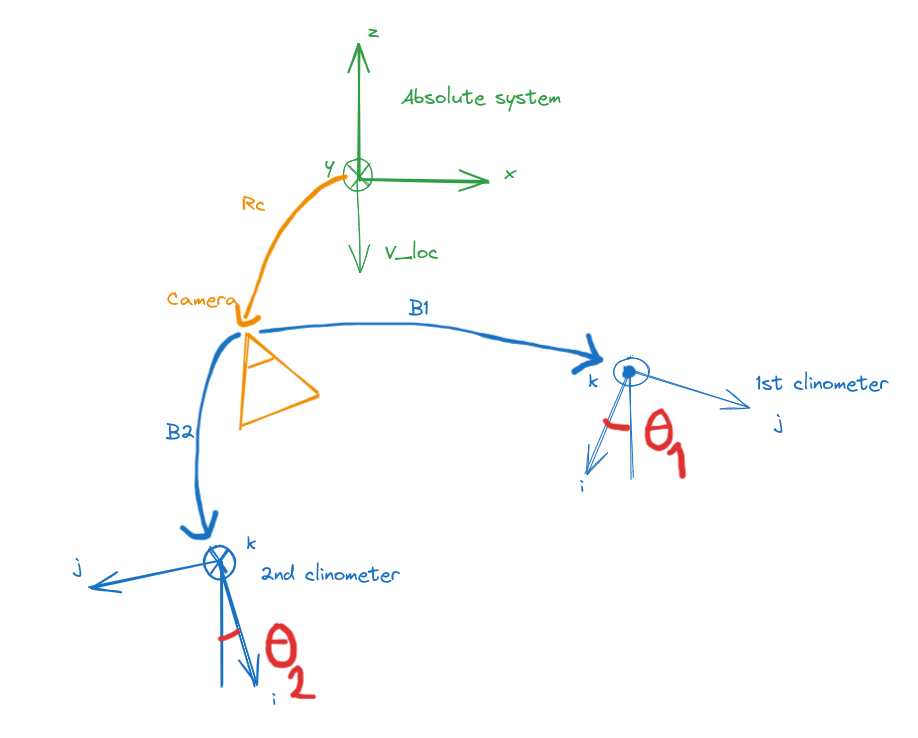
\includegraphics[width=12cm]{Programmer/ClinoBA.png}


\subsection{Clinometers measures file}

The file with clinometers measures must have :
\begin{itemize}
     \item one line per camera
     \item in each line, the image name
     \item in each line, the measures of the clinometers
     \item each clinometer measure has the name of the clinometer, its measure and its sigma  
\end{itemize}

For example, the file should be like :

\begin{lstlisting}
image1 clino1 +0.064786 +0.00001 clino2 +0.014629 +0.00002
image2 clino1 +0.064786 +0.00001 clino2 +0.014629 +0.00002
image3 clino1 +0.064786 +0.00001 clino2 +0.014629 +0.00002
\end{lstlisting}


\subsection{ImportMeasuresClino}

First step is to import clino measures.

\begin{lstlisting}
     MMVII ImportMeasuresClino ClinoValue.txt "ImNASNASNASNAS" clinoMeasures [043_,.tif]
\end{lstlisting}

Parameters of {\tt ImportMeasuresClino} are :
\begin{itemize}
     \item ClinoValue.txt : file with clinometers measures.
     \item "ImNASNASNASNAS" : structure of ClinoValue.txt : Im for image name, N for clinometer name, A for clinometer measure, S for sigma measure
     \item clinoMeasures : directory with the imported values : MMVII-PhgrProj/MeasureClino/clinoMeasures
     \item $[$043$\_$,.tif$]$ : values added before and after image names in ClinoValue.txt to have the correct names of camera
\end{itemize}


\subsection{ClinoInit}

The first step is to find approximation of the Boresight matrixes with {\tt ClinoInit}.

\begin{lstlisting}
     MMVII ClinoInit clinoMeasures [1,0] BA_Br INIT_CLINO Rel12="i-kj"
\end{lstlisting}


Parameters of {\tt ClinoInit} are :
\begin{itemize}
     \item clinoMeasures : directory with imported clinometers measures
     \item $[$1,0$]$ : index of clinometers to use
     \item BA$\_$Br : orientation of camera
     \item INIT$\_$CLINO : name of directory where approximation of clinometers calibrations will be saved
     \item Rel12="i-kj" : an approximation of the relative orientation between the two clinometers systems ($\Vec{i_2}=\Vec{i_1}, \Vec{j_2}=-\Vec{k_1}, \Vec{k_2}=\Vec{j_1}$)
\end{itemize}

In INIT$\_$CLINO, there are the clinometers name with their approximate Boresight matrix. There is also the approximation of the relative orientation between the two clinometers system.



\subsection{OriBundleAdj}

Then, you can compute the Boresight matrixes with {\tt OriBundleAdj}. You need to complete the parameter ClinoDirIn to compute the clinometers calibration

\begin{lstlisting}
     MMVII  OriBundleAdj  AllImClino.xml  BA_Br   BA_Clino   GCPDir=Clino_Filtered  GCPW=[1,0.1]  PPFzCal=.* ClinoDirIn=INIT_CLINO ClinoDirOut=CALIB_CLINO InMeasureClino=clinoMeasures
\end{lstlisting}

Parameters of {\tt ClinoInit} are :
\begin{itemize}
     \item AllImClino.xml : name of images
     \item BA$\_$Br : orientation of camera
     \item BA$\_$Clino : orientation of camera after the bundle adjustment
     \item GCPDir=Clino$\_$Filtered : directory for GCP
     \item GCPW=[1,0.1] : GCP weights
     \item PPFzCal=.* : freeze internal calibration
     \item ClinoDirIn=INIT$\_$CLINO : approximation of the two Boresight matrixes computed with {\tt ClinoInit}
     \item ClinoDirOut=CALIB$\_$CLINO : name of directory where clinometers calibrations will be saved
     \item InMeasureClino=clinoMeasures : directory with imported clinometers measures
\end{itemize}

The output clinometers orientations are the same than for {\tt ClinoInit}.


\part{Annexes}

\appendix

\chapter{Bibliography}


\begin{thebibliography}{AAA}
   \bibitem[Tomasi Kanabe 98]{TomKan}   S. Roy, I.J. Cox , 1998, "Shape and Motion from Image 
            Streams under Orthography: a Factorization Method", International Journal of Computer Vision, 
            9:2, 137-154 (1992)


    \bibitem[CERES]{CERES} \emph{https://github.com/ceres-solver/ceres-solver/blob/master/include/ceres/jet.h}

    \bibitem[CODED Target]{CircCodeTarget} \emph{https://www.isprs.org/proceedings/xxix/congress/part5/56\_xxix-part5.pdf}

   \bibitem[Cox-Roy 98]{CoxRoy}   S. Roy, I.J. Cox , 1998, "A Maximum-Flow
            formulation of the N-camera Stereo Correspondence
      Problem", \emph{Proc. IEEE Internation Conference on
      Computer Vision}, pp 492--499, Bombay.

   \bibitem[Fraser C. 97]{Fraser}  C. Fraser, 1997, "Digital camera self-calibration",
   \emph{ISPRS Journal of Photogrammetry and Remote Sensing}, vol. 52, issue 4, pp. 149-159,
   \bibitem[Penard L. 2006 ]{Penard}   L. Pénard, N. Paparoditis, M. Pierrot-Deseilligny.
           "Reconstruction 3D automatique de façades de bâtiments en multi-vues.",
            RFIA (Reconnaissance des Formes et Intelligence Artificielle),
            Tours, France, January 2006.

    \bibitem[Weierstrass,Karl 1885 ]{Weierstrass1885} Über die analytische Darstellbarkeit sogenannter willkürlicher Functionen
           einer reellen Veränderlichen. Sitzungsberichte der Königlich Preußischen Akademie der Wissenschaften zu Berlin,
           1885 (II).  Erste Mitteilung (part 1) pp. 633–639, Zweite Mitteilung (part 2) pp. 789–805.

    \bibitem[Stone, M. H. 1937]{Stone1937} "Applications of the Theory of Boolean Rings to General Topology",
          Transactions of the American Mathematical Society, Transactions of the American Mathematical Society,
          Vol. 41, No. 3, 41 (3): 375–481

\end{thebibliography}


\printindex



\end{document}




